
% document type
\documentclass{uonmathreport}

% packages
\usepackage[pdftex]{graphicx}
\bibliographystyle{abbrv}
\usepackage{hyperref}
\usepackage{tikz}
\usepackage{listings}
\usepackage{minted}
\usepackage{caption}
\usepackage{pdfpages}
\usepackage{subfig}

% change to \PJS or \DIS or \HGDIS (for BSc and MPhil)
% or \MSc (for all Msc dissertations)
\MSc

% adjust the following
\title{Numerical Computations of Neural Field Models on Triangulated Meshes}
\author{Giordi Azonos Beverido}
\academicyear{2016/17}
\supervisor{Dr. Daniele Avitabile}

% the following are irrelevant for Msc:
\assessmenttype{Review} % or Investigation
\projectcode{XX P99}

% the following are irrelevant for PJS, PJA, DIS and HG4DIS:
% Msc: change it to G1PMD and Pure Mathematics, etc ...
\msccode{G14SCD}
\msctitle{Scientific Computation}

% gives double-spacing
\linespread{1.6}
% the margins are set automatically. Do not make them smaller.

% put your own definitions and shorthands here
\newcommand{\ZZ}{\mathbb{Z}}
\captionsetup[figure]{font=footnotesize,labelfont=footnotesize, skip=0pt}
\captionsetup[table]{font=footnotesize,labelfont=footnotesize}
\captionsetup[listing]{font=footnotesize,labelfont=footnotesize, skip=0pt}
\setminted{fontsize=\small,baselinestretch=1}

\begin{document}

\maketitle

%----------------------
\begin{abstract}
Neural field models are tissue-level models that describe the dynamics of large-scale neural networks by means of a continuous non-linear integro-differential equation. Throughout this work we develop numerical methods for solving neural field equations in one and two dimensions. Particularly, we develop a method for solving neural field equations on a triangulated mesh. We view the right hand side of the neural field equation as a Fredholm integral equation of the second kind, and thus, use Nystr\"om method with a Gaussian quadrature rule on triangulated meshes to discretize the equation in space, and then evolve it forward in time with a Runge-Kutta4 algorithm to find localised states and patterns of activity. Additionally we develop object oriented code in python to solve different instances of the neural field equation using Fast Fourier Transform methods and Nystr\"om method.
\end{abstract}

%-----------------------
% Table of contents
\setcounter{tocdepth}{2}  % this will list subsections, but not subsubsections
\tableofcontents 

%--------------------------------------
\newpage
\section{Introduction} \label{sec:intro}

Neural field models are tissue-level models that describe the average activity of spiking neurons. They model the dynamics of large-scale neural networks by means of non-linear integro-differential equations, where the neuronal synaptic connections are captured with an integral kernel, and single neuron spikes with a continuous ``firing rate" function. 
They can be classified as either activity-based or voltage-based models.

The amount of neurons even in small cortical regions is very dense, and simulations of networks comprised of thousands of spiking neurons requires working with huge matrices and storing huge amounts of information, which makes computations and analysis intractable when trying to simulate neural systems with spiking neurons on the scale of functional units in the brain. The objective of Neural Fields is to establish continuous equations based on descriptions that do not take the individual spikes of neurons into account, but instead describe the average activity of spiking neurons or neural populations, and treat cortical space as continuous, giving rise to models described by integro-differential equations.

The current approach to neural field models is based on the work of Wilson and Cowan \cite{wilson1972excitatory,wilson1973mathematical} and Amari \cite{amari1975homogeneous,amari1977dynamics}. 
A typical Amari type equation focuses on local excitation and distal inhibition, which models a mixed population of interacting inhibitory and excitatory neurons with typical cortical connections, where the rate of change of activity $u$ at position $x$ and time $t$ depends on the influence of neighbouring $u$ at all other positions $y$. Such a model is represented mathematically by:
\begin{equation}\label{eqn:amari_nf}
\frac{\partial u(x,t)}{\partial t} = -u(x,t) + \int_{D} W(x - y)f(u(y,t))dy, \hspace{5mm} D \subset \mathbb{R}^m, m = 1,2,3.
\end{equation}
where $W(x - y)$ is the kernel function which quantifies the interactions between a population of neurons at position $y$ and its neighbouring population at position $x$. A typical form assumes that the influence depends only on the distance from $x$ to $y$. The function $f(u)$ is referred to as the firing rate function and describes the average spiking behaviour of the population of neurons. A detailed description of how this models may give rise is included in section \ref{subsec:Modelling the average behaviour of neurons}. It is often assumed that the interaction tends to zero for $|x - y|$ large and that this interaction is spatially symmetric; that is:
\begin{equation}
W \rightarrow 0 \hspace{4mm} \textnormal{as} \hspace{4mm} |x - y| \rightarrow \infty, \hspace{4mm} \textnormal{and} \hspace{4mm}W(x - y) = W(|x - y|)
\end{equation}
If $W$ tends to zero quickly, then the long range effects are weak, otherwise they are strong.

A kernel that incorporates short range interactions and long range inhibition is described by a ``Mexican-hat" function. It has been shown that any population of neurons will contain a subpopulation of both excitatory and inhibitory neurons, and that complex neural processes rely on the interaction of these two sub populations \cite{wilson1972excitatory}, making this a more realistic choice. See Figure \ref{fig:kernls}.b. Another kernel that does not incorporate inhibitory behaviour is that of a ``Wizard Hat" function. This is, any two neurons excite each other, but with an ‘excitatory strength’ that decays exponentially the further apart they are. See Figure \ref{fig:kernls}.a

\begin{figure}
	\begin{center}
		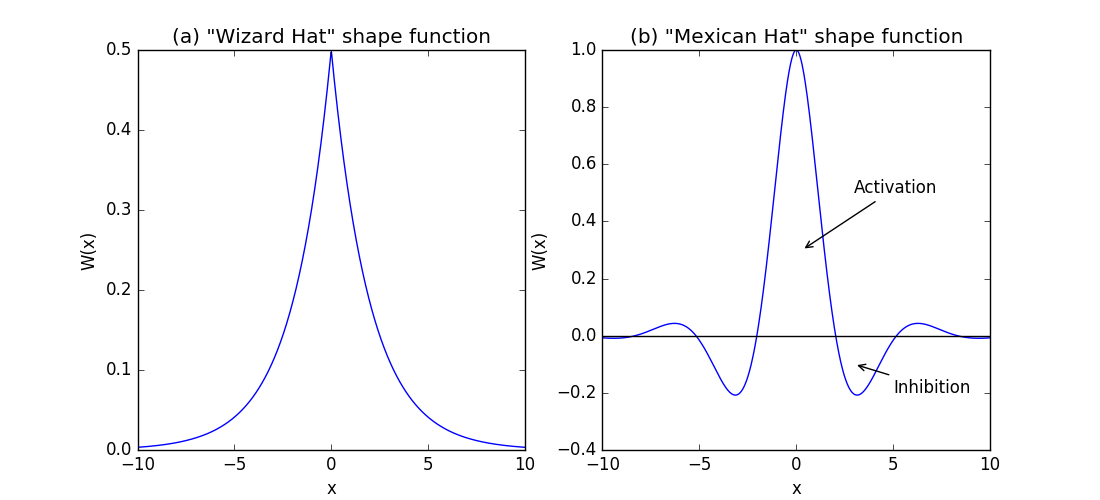
\includegraphics[width=1\textwidth]{Figures/Kernels.png}
	\end{center}
	\caption{Two choices for the Kernel Function}
	\label{fig:kernls}
\end{figure}

Since the pioneering work of Wilson, Cowan and Amari, Neural Field models have helped understanding a variety of Neuronal Phenomena such as geometric visual hallucinations \cite{bressloff2001geometric}, motion perception \cite{giese2012dynamic}, autonomous robotic behaviour \cite{erlhagen2006dynamic}, anaesthesia \cite{liley2011mesoscopic} and epileptic seizures \cite{milton2013epilepsy}, between much others.
A lot of progress in Mathematical and Computational approaches has been achieved leading to results such as the existence and uniqueness of bumps \cite{kishimoto1979existence} and waves \cite{bressloff2014waves} with smooth sigmoidal firing rates, geometric singular perturbation analysis, numerical bifurcation techniques to analyse solutions in one spatial dimension \cite{laingatwo,pinto2001spatially,AVITABILE201524,rankin2014continuation} and results from one to two spatial dimensions \cite{coombes2012interface,folias2004breathing,laing2003pde,owen2007bumps,lima2015numerical}, between much more. For a more complete overview of the work done in Neural Fields, as well as a deeper understanding of this discipline, I refer the reader to \cite{coombes2012NeuralFields}.

The Amari type neural field model as the one in eqn.\ref{eqn:amari_nf} has been analytically and numerically studied on flat surfaces or flat domains. On those cases the distance between two points, which is required to compute the connectivity kernel $W$, is well defined and thus, progress can be made to understand the origin of a wide variety of activity patterns. However, the brain is not flat. Sculped on the cortical surface are characteristic bumps and grooves known as gyri and sulci. Thus, it is necessary to develop numerical techniques that can solve the neural field equation on a surface that more closely resembles the actual shape of a brain.  Perhaps, one possible approach is to cover the brain surface with triangular elements so that we can reproduce this bumps and grooves and have a non-flat surface that resembles the actual shape of a brain and where we can numerically solve the neural field equation.

In this work we take a first step towards that objective by developing a numerical algorithm that solves the neural field equation \ref{eqn:amari_nf} on a two dimensional triangulated mesh. The purpose is that the algorithms developed here can be recovered to work on triangulated surfaces that more closely resemble the actual shape of a brain. A secondary, yet not less important objective, is to develop generic, understandable and well written code in an object oriented way to solve different instances of the neural field equations with varying initial conditions and parameters, so that any one with a slight understanding about neural fields can use and modify to produce solutions using different connectivity kernels $W$ and firing rate functions $f$. This code will be kept on a private GitHub repository named: \texttt{danieleavitabile/giordi-azonos-msc-dissertation}, for access contact the supervisor of the work.

The neural field equation \ref{eqn:amari_nf} is a time dependant integro-differential equation. A common strategy to derive numerical results of equation \ref{eqn:amari_nf} is to first discretize the right hand side of this equation in space, and then use time stepping techniques to evolve it forward in time. Throughout this work we extensively use Nystr\"om method with a Gaussian quadrature rule to discretize the right hand side of equation \ref{eqn:amari_nf} in space, and then use a Runge-Kutta4 algorithm to evolve the equation forward in time. Although there are more efficient ways to discretize the right hand side of the neural field equation like, for instance, Fast Fourier Transform methods, we needed a technique capable of working on triangulated meshes. As will be seen later, Nystr\"om method was developed to compute approximations of integral equations based on numerical integration of the integral operator in the equation, and Gaussian quadrature turns out to be a very efficient quadrature technique that can be used for numerical integration on triangulated meshes. Therefore we decided to develop numerical algorithms based on Nystr\"om method with a Gaussian quadrature rule.

The code was developed using Python 3.5\footnote{https://www.python.org} with Anaconda\footnote{https://www.continuum.io/downloads} distribution. For each case, a python Juypter notebook with explanatory notes is available, as well as a python script runnable from a terminal. Code is available on a private GitHub repository named: \texttt{danieleavitabile/giordi-azonos-msc-dissertation}, for access contact the supervisor of the work. For numerical computations we used \texttt{numpy} and \texttt{scipy} packages, for plotting we used \texttt{matplotlib} and for building triangulated meshes we used \texttt{meshpy}\footnote{https://mathema.tician.de/software/meshpy/}.  

The Code on GitHub is available for the following cases, using the following techniques:
\begin{enumerate}
	\itemsep-0.5em
	\item One dimensional case: Nystr\"om method with Composite Trapezoidal rule, 1D Fast Fourier Transform method.
	\item Two dimensional case: Nystr\"om method with Gaussian quadrature, 2D Fast Fourier Transform method.
	\item Two dimensional case on a triangulated mesh: Nystr\"om method with Gaussian quadrature.
	\item Two dimensional case with adaptation: Nystr\"om method with Gaussian quadrature, 2D Fast Fourier Transform method.
\end{enumerate}

This work is organized as follows: The second chapter will introduce the reader to the theory of neural field modelling. We start by giving a biological background of how synapses between single neurons work and then explain how modelling a population of spiking neurons on a cortical region may give rise to neural field models. 

The third chapter gives a quick survey of the numerical techniques that have been used to solve neural field equations, as well as their numerical properties. Particularly, we look at Projection methods, Nystrom method, Fast Fourier Transfom methods and PDE methods which transform the integral equation to a Partial differential equation. 

Chapter four will solve a one dimensional neural field equation using Nystr\"om method. It starts explaining how Nystr\"om method can be used to discretize this particular instance of the problem, and then presents some results in the form of localised bump solutions.

On chapter five we develop a numerical method for solving a two dimensional neural field equation on a tensor-product grid using Nystr\"om method with a Gaussian quadrature rule. The section starts explaining how Nystr\"om method with Gauss interior points can be used to discretize this particular instance of the problem. Then discusses the computational implementation of the method by presenting some pieces of code and key functions to generate the algorithm. We perform numerical tests to the method by studying the error behaviour on pre-built cases where we know the exact solution before hand. Finally, we validate the method by reproducing results obtained in previous studies. Particularly, we compute convergent and divergent spot solutions.

On chapter six, we extend the work of chapter four by developing a numerical method for solving a two dimensional neural field equation on a mesh consisting of triangular elements using Nystr\"om method with a Gaussian quadrature rule. The sections starts by introducing a Gaussian quadrature rule that works on single triangular elements, then it is extended for a whole triangulated mesh. After this we use the developed quadrature rule to discretize the equation on a triangulated mesh using Nystr\"om method. The method is tested by studying the error behaviour on pre-built cases where we know the exact solution before hand. Finally, we validate the method by reproducing the results obtained in chapter five as well as in previous studies.

Chapter seven is an application of the algorithm developed on chapter six to another instance of the neural field equation. Namely, a two dimensional neural field with linear adaptation. We present the results obtained by computing the convolution integral using a Fast Fourier Transform method on a tensor-product grid, and compare them with the results obtained with Nystr\"om method on a triangulated mesh.

The eight chapter contains the main python script, in Jupyter Notebook format, for solving the Neural Field equation on a triangulated mesh step by step. Finally, the ninth chapter will review the results and provide conclusions.

On the Appendix Code section we include relevant pieces of code on python language for implementing the algorithms developed throughout the report and the key classes necessary for running the object oriented main files on the GitHub account.

Throughout the report we found two possible approaches to evaluate the right hand side of the neural field equation using Nystr\"om method with Gaussian quadrature. One is by means of for loops, iterating through each point in the grid at each time evaluation. With this approach, each evaluation of the right hand side takes $O(N^2)$ operations, where $N$ is the total number of points in the grid. We found that, for more refined grids ($N\rightarrow \infty$), the algorithm becomes extremely slow. That is due to the number of right-hand side evaluations being performed and the complexity of each evaluation. Each time step, the RK4 algorithm requires four evaluations of the right-hand side, each costing $O(N^2)$ operations. A second approach, and the one we used to develop the methods, is to pre-build a ``Synaptic Matrix" $\textbf{W}$ that holds the interactions between neurons mediated by the Connectivity Kernel function $W(x_i,x_j) \hspace{2mm} \forall i,j$, and then evaluate the right-hand side by matrix-vector multiplication. This approach proved to be faster and to support finer grids due to the efficiency of python's \texttt{numpy} package when performing matrix-vector multiplications. Even though time stepping is faster using matrix-vector multiplications, it still takes a lot of time to assemble the synaptic matrix. Although, by exploiting the symmetry of the Connectivity Kernel, in the sense that $W(x,y) = W(|x,y|)$, and python's \texttt{numpy} package efficiency, we devised a strategy that halves the time it takes to assemble the full matrix $\textbf{W}$ by computing the values for the upper triangular part of $\textbf{W}$, and then use \texttt{numpy} to efficiently copy the values of the upper triangular to the lower triangular part of $\textbf{W}$. A huge drawback from working with matrices is that an additional $O(N^2)$ memory is required to store the matrix. Besides, for more refined grids, or too big domains, this approach also becomes inefficient and time consuming. Particularly, the convergence of spot solutions is found to be extremely sensitive to grid discretizations and thus, a very fine grid is needed to accurately compute solutions of neural field models. Therefore, there is a need for methods that can handle faster right hand side evaluations of the system, and that can perform efficiently on finer grids. A possible solution, and hence an extension of this work, might be to implement the for loop strategy using parallel algorithms.

%---------------------------------------
\newpage
\section{Neural Field Modelling}\label{sec:nf modelling}
This chapter explains how, starting from single spiking neurons, neural field models may give rise. It first gives a biological background and an overview of the basic functionality of synapses between single neurons, and then explains how, by modelling populations of spiking neurons, one can get a neural field equation as the one in \ref{eqn:amari_nf}.
\subsection{Single Neurons and Synapses}\label{subsec:single_neurons}
We give a basic and general overview of how single neurons and synapses between them work by summarizing parts of the work presented in \cite{CompNeuroSci}, Part I. For a more in depth explanation of how synapses between single neurons are modelled mathematically I refer the reader to \cite{CompNeuroSci,bressloff2011spatiotemporal,bressloff2014waves}.
\subsubsection{Structural Properties of Neurons}\label{subsubsec:neurons_properties}
Cortical Neurons are the processing units of the brain. They are cells, so they have a \textit{Nucleus} containing DNA, \textit{Ribosomes} which assemble proteins from genetic instructions, and a \textit{Mitochondria} that provides energy. However, the most important parts of the neuron, for us, are the \textit{Cell Body} (or Soma), the branching \textbf{output} structure known as the \textit{Axon}, and the branching \textbf{input} structure known as the \textit{Dendritic Tree}. In a very general overview, Neurons communicate between them by sending action potentials (electrical impulses) along their Axons. Axons are ``connected" to Dendrites of other neurons via microscopic junctions known as \textit{Synapses}. Each neuron receives electric impulses from many other neighbouring neurons through its \textbf{input} Dendritic Tree, if the accumulated electric input received from all the Synapses reaches some threshold, the neuron spikes or fires, and a pulse of fixed strength and duration travels through the body, and is \textbf{outputted} through the Axon, which eventually gets to another neuron.
The Axon can not only communicate to neurons in neighbouring areas, but they can also reach through white matter to other neurons, making communications possible from other than nearest neighbours, that is, long range interaction. Such \textbf{input} can be positive, which induces activity, or negative which inhibits it.

Synapses are the most important phenomenon for information-processing inside neurons. Basically, a synapse enables signals from a presynaptic neuron to alter the state of the postsynaptic neuron, which in turn triggers the generation of an electric pulse (spike), or a train of spikes in the postsynaptic neuron. Hence, we shall concentrate on understanding how synapses work.

\subsubsection{Membrane Potential}\label{subsubsec:membrane_pot}

The ability of a neuron to vary its membrane potential is important for the information transmission of a neuron. The membrane potential, which we shall denote by $V$, is defined as the difference between the electric potential inside a cell and the electric potential outside. This potential difference arises from a difference in the concentration of ions inside and outside the cell. The important part of the membrane potential is that, depending on the neuron functionality, it can be altered to transmit information. For example, photoreceptor cells in the retina convert light into signals that alter the membrane potential of photoreceptor neurons.

The most common type of connection between neurons in the central nervous system is the chemical synapse. To understand how membrane potentials are modelled mathematically, it is necessary to understand chemical synapses. Particularly, ion channels and neurotransmitters. 

\subsubsection{Ion Channels}\label{subsubsec:ion_chan}
Chemical synapses and consequently, information transmission between neurons is largely based on ion channels. 
Ion channels are special types of proteins embedded in the membrane of a neuron, these proteins form pores that enable specific ions to enter or to leave the neuron. There are three important ions in the neurons: Sodium $Na^+$, Calcium $Ca^{2+}$ and Potassium $K^+$. Additionally, there are different types of ion channels which can be open or close allowing ions to enter or leave the neuron. The ion channels that drive the resting potential of neurons are the leakage channels, which are usually open all the time. An ion channel being open or close depends on certain chemical factors surrounding the neuron. A usual mathematical approach for modelling ion channels involve probabilities of ion channels being open or close. 

\subsubsection{Chemical Synapses and Neurotransmitters}\label{subsubsec:neurotrans}

Neurotransmitters, also known as \textit{chemical messengers}, are special chemicals that transmit signals across chemical synapses from one neuron to another. They are released from \textit{synaptic vesicles} in synapses into the \textit{synaptic cleft} (a very small gap between the axon terminal and the dendrite of the postsynaptic neuron), where they are received by receptors on the postsynaptic neuron. They play a major role on how the brain works, how people learn, etc. For example, Dopamine (DA) is one neurotransmitter that plays a crucial role in motivation, attention, and learning. There are hundreds of other Neurotransmitters in the brain.

Neurotransmitter-gated ion channels, formally known as Ligand-gated ion channels are a group of ion channels which open in response to the binding of a chemical messenger, such as a neurotransmitter. This, in turn, results in either a \textit{depolarization}, for an excitatory receptor response, or a \textit{hyperpolarization}, for an inhibitory response. When this ion channels open, ions flow through them, changing the membrane potential of the postsynaptic neuron. The response in the membrane potential is called the postsynaptic potential (PSP). A larger amount of neurotransmitter released by the presynaptic neuron causes a bigger response in the postsynaptic membrane potential, but the relationship is not linear.

\subsubsection{Conductance based model of a neuron}\label{subsubsec:conduc_model}

The variation of a membrane potential from a presynaptic spike can be described as a postsynaptic potential (PSP). 
An excitatory synapse is one in which the membrane potential is increased, we call this excitatory postsynaptic potential (EPSP). On the other hand, inhibitory postsynaptic potentials (IPSPs) are responses that lower the membrane potential.

A prototypical form of action potential (spike) was measured in the giant axon of a squid by \textit{Alan Hodgin} and \textit{Andrew Huxley} \cite{hodgkin1952quantitative}. It is caracterized by a sharp increase of the membrane potential to positive values, followed by a sharp decrease in the membrane potential know as post-synaptic depression.

The fact that they quantified the process leading to the generation of action potentials with mathematical terms that were later identified with ion channels was a major scientific accomplishment by Hodgkin and Huxley which caused them to win a Nobel prize in 1963.

They saw the brain as a big battery consisting of a capacitor in parallel with three resistors (ion channels), each supplied with their own battery setting their reversal potential. One of the resistors is constant (leakage), while the other two can change depending on the state of the system ($Na^+$, $K^+$). The combined effects of the different components can be expressed by means of the conservation of electric charge (\textit{Kirchoff's Current Law}):
\begin{equation}
C \frac{dV(t)}{dt} = - I_{con} + I_{syn} + I_{ext},
\end{equation}

where $C$ is the cell capacitance, $I_{con}$ is the membrane current (the minus sign here is used to measure current flow from outside the cell to the inside), $I_{syn}$ denotes the sum of synaptic currents entering the cell, and $I_{ext}$ is an external current entering the cell.

As seen in \cite{bressloff2011spatiotemporal}, the membrane current through an ion channel varies  with changes in the membrane potential $V$ in relation to some reversal potential that mediates the synaptic current. Summing over all ion channel types, the total membrane current leaving the cell through the cell membrane is:
\begin{equation}
I_{con} = \sum_s g_s(V - V_s),
\end{equation}

here $g_s$ is the conductance due to ion channel of type $s$ and $V_s$ is the corresponding reversal potential. The conductance $g_s$ for ion channels of type $s$ is taken to be the product $g_s= \bar{g}_sP_s$ where $\bar{g}_s$ is equal to the density of channels in the membrane multiplied by the conductance of a single channel and $P_s$ is the fraction of open channels.

\subsubsection{Synaptic Processing}\label{subsubsec:syn_process}

As mentioned in Section 2.1.4, when a spike arrives at the Axon of a presynaptic neuron, it causes $Ca^+$ ion channels to open. This produces a saturation of $Ca^+$ which in turn causes synaptic vesicles containing neurotransmitters to release their content into the synaptic cleft and bind to receptors on the Postsynaptic membrane. The binding causes ion channels to open (or close) which in turn, changes the ability of ions to flow through the postsynaptic membrane. Hence, the binding of neurotransmitters alters the conductance of the postsynaptic membrane. The response of the membrane potential is known as the Postsynaptic potential (PSP).

According to \cite{bressloff2011spatiotemporal} section 2.2, a single synaptic event due to the arrival of an action potential at time $T$ induces a synaptic current of the form:
\begin{equation}\label{eqn:individual_response}
I_{syn}(t)=g_{syn}(t - T)(V_{syn} - V(t)),
\end{equation}

where $V$ is the voltage of the postsynaptic neuron, $V_{syn}$ is the synaptic reversal potential and $g_{syn}(t)$ is the change in synaptic conductance. The sign of $V(t)$ relative to the resting potential (assumed to be zero) determines whether the synapse is excitatory ($V(t) > 0$) or inhibitory ($V(t) < 0$).

A common choice for $g_{syn}(t)$ is a difference of exponentials:
\begin{equation}
g_{syn}(t) = \bar{g}(\frac{1}{\alpha} - \frac{1}{\beta})^{-1}
(e^{-\alpha t} - e^{-\beta t})H(t),
\end{equation}
or the $\alpha$ function:
\begin{equation}
g_{syn}(t) = \bar{g} \alpha^2 t e^{-\alpha t}H(t),
\end{equation}
where $H(t)$ is the Heaviside function, $\bar{g}$ a constant conductance, and $\alpha$,$\beta$ are time constants describing the rise and fall of the synaptic response respectively.

For simplicity we will study the case where the rise time dominates the fall time, that is, $\beta \ll \alpha$, which leads to the exponential synapse
\begin{equation}\label{eqn:exp_synapse}
g_{syn}(t) = \bar{g} e^{-t/\alpha}H(t),
\end{equation}
we also assume that a neuron spends most of its time close to rest, so that $V_{syn} - V \approx V_{syn}$, with the factor $V_{syn}$ being absorbed into $g_{syn}$, then we are now taking the arrival of a spike as generating a synaptic current rather than a change in conductance.

We now have that a synaptic current arising from a train of action potentials can be approximated by summing the individual responses \ref{eqn:individual_response}, giving the total synaptic input, which we denote by $u(t)$, as
\begin{equation}\label{eqn:train_spikes}
u(t) = \bar g \sum_m g_{syn}(t-T_m).
\end{equation}
As expressed in \cite{coombes2012NeuralFields} section 1.1.1, and taking the exponential synapse as in \ref{eqn:exp_synapse}, we note that the form for $g_{syn}$ can be expressed as a function of a linear differential operator, such that $Qg_{syn}(t) = \delta(t),$ where
\begin{equation}
Q = (\frac{d}{dt} + \frac{1}{\alpha}),
\end{equation} 
with inverse kernel $\Phi(t) = H(t)e^{-t/\alpha}.$

\subsection{Modelling the average behaviour of neurons}\label{subsec:Modelling the average behaviour of neurons}

As already mentioned, simulating networks comprised of thousands of spiking neurons requires working with huge matrices and storing huge amounts of information, which makes computations and analysis very complicated for an increasing amount of neurons. Based on the work of \cite{coombes2012NeuralFields,bressloff2011spatiotemporal,CompNeuroSci}, this section explains how neural field models arise by taking tissue-level averages of single spiking neurons, and under what conditions are these approximations faithful and useful for modelling neural activity in cortical regions.

\subsubsection{Firing Rate functions}
\label{subsubsec:firing_rate_functions}

For Neural population models, action potentials are described by a continuous function rather than single spikes. These continuous function is called the firing rate function. A continuous firing rate function is derived by estimating the average temporal spike rate of a single neuron within a fixed window $\Delta t$. As described in the book \cite{CompNeuroSci} section 3.4.1, such an average is given by
\begin{equation}\label{eqn:time_average}
 \langle f \rangle_t = \frac{\text{\# of spikes in} \Delta t}{\Delta t} = \frac{1}{\Delta t}\int_{t-\Delta t/2}^{t+\Delta t/2} \delta(t - T) dt, 
\end{equation}
where $T$ is the firing rate time of the neuron. This defines, for small time windows, the \textit{instantaneous firing rate} function. For actual neuron behaviour, spikes vary widely from one another, so in order for this approximation to be accurate, we need to assume that the average is performed over small varying inputs, which means that spikes don't vary widely over the chosen time window $\Delta t$.

As in \cite{coombes2012NeuralFields} section 1.2, we see how this fits with the Synaptic Processing models from section \ref{subsubsec:syn_process}. Recall that the conductance change arising from a train
of spikes, is given by \ref{eqn:train_spikes}. Writing this equation in its equivalent form
\begin{equation} \label{eqn:escrom}
Qu(t) = \bar g \sum_m \delta(t-T_m),
\end{equation}
performing a short-time average of \ref{eqn:escrom} over a time scale $\Delta t$ and assuming $g_{syn}$ is sufficiently slow so that $\langle Qu \rangle_t$ is approximately constant, then we have that $Qu = f$, with $f$ being the instantaneous firing rate function.

\subsubsection{Population Models}
\label{subsubsection:Population Models}

It would be naive to rely on the information of a single spike train for describing the behaviour of a big amount of neurons contained in a cortical region. Hence, we also assume that there is a subpopulation or pool of neurons with similar response properties firing asynchronously. This means we are essentially reinterpreting the activity variables $u$ and $g_{syn}$ as mean fields of local populations.

Thus for a single population with self-feedback we are led to equations of the form:
\begin{equation}
Qu(t) = w_0f(g),
\end{equation}
for some strength coupling $w_0$

As expressed in \cite{coombes2012NeuralFields} section 1.2. We can extend the model to a tissue level model by posing $u = u(x,t)$ over a spatial domain $x \in D$, with $D \subset \mathbb{R}^m, m = 1,2,3$. Furthermore, we introduce a coupling function $W(x,y)$ to describe the interaction of neurons over the continuum, and integrate over the domain $D$ to obtain
\begin{equation}
Qu = \int_{D} W(x,y) f(u(y,t)) d\sigma(y),
\end{equation}
where we denote $\sigma(y)$ as the measure of the domain $D$ with respect to $y$, or equivalently
\begin{equation} \label{eqn:nf_voltageBased}
\frac{\partial u(x,t)}{\partial t} = -u(x,t) + \int_{D} W(x,y) f(u(y,t)) d\sigma(y) + I_{ext}(x,t), \hspace{5mm} D \subset \mathbb{R}^m, m = 1,2,3,
\end{equation}
where $I_{ext}(x,t)$ is an added external input which, when not included, will be assumed as $I_{ext} = 0$.
 
This is also known as the Voltage-based model. Another instance of this model is the Activity-based model. A derivation of the Activity-based model is given in \cite{bressloff2011spatiotemporal}, chapter 2. In this work we focus on solving equation \ref{eqn:nf_voltageBased} for the cases where $m = 1,2$; and then extend the 2 dimensional case to solve it for more complicated triangulated domains.

When $m=1$, we have that $D = \mathbb{R}$, this stands for the case where we deal with a one-dimensional set of neurons. The physical interpretation of this model is that $u(x,t)$ is the average voltage of a large group of neurons at position $ x \in \mathbb{R}$ and time $t$. The interaction between neurons is measured with the one-dimensional distance between them, that is, $W(|x-y|)$. Although its limited biological interest, it is a very important case because of the insights one can get from studying this models. For a review of the dynamics in neural field models, particularly in 1D, see \cite{coombes2005waves}.

When $m=2$, then $D = \mathbb{R}^2$, and we deal with two-dimensional sets of neural fields. The physical interpretation of this model is that $u(\mathbf{r},t), \mathbf{x} \in \mathbb{R}^2$ is the average voltage of a dense group of neurons positioned at $\mathbf{r} = (x,y)$ in a cortical region. In this case, the interaction between groups of neurons is measured with the Euclidian distance $\| \cdot\|_2$ i.e. $W(\|\mathbf{r}- \mathbf{r}' \|_2)$. This is, perhaps, a more biologically realistic model, since the domain can now be viewed as a piece of cortex where the thickness is neglected. Particularly, the mammalian cortex is often regarded as a two dimensional sheet of densely interconnected neurons. Examples of research developed on this models include \cite{owen2007bumps,rankin2014continuation,laing2003pde,laingatwo,coombes2014spots}. 

For the case when $m=3$, we talk about neural fields in which $D$ is a two-dimensional manifold embedded in $\mathbb{R}^3$. One example of work on this area is \cite{visser2017standing}. Although not much has been explored in this path, it is an important case because the brain has a three-dimensional shape, and interactions between neurons occur on the two-dimensional non flat manifold surface. In this case the interaction between neurons might be mediated by the geodesic distance defined as the shortest path between two points.

Other instances of eq. \ref{eqn:nf_voltageBased} incorporate mechanism such as synaptic depression/facilitation, spike frequency adaptation \cite{ermentrout2014spatiotemporal,coombes2003waves,coombes2014spots,laingatwo} and axonal propagation delays.

\section{Survey of Numerical Methods}\label{sec:numerical_methods}
There exist a variety of methods for numerically solving the Amari type integral equation \ref{eqn:amari_nf}. In this section we will look at some of the numerical methods available, and their theoretical properties. In particular, we look at how the right hand side of \ref{eqn:amari_nf} can be viewed as a Fredholm integral equation of the second kind, and thus, look at Projection methods and Nystr\"om methods. We also look at other methods that don't use this fact, such as Fast Fourier Transform methods, and PDE methods.

As stated in eq.\ref{eqn:amari_nf}, the synaptic activity of a population of neurons over a finite sized cortical region can be described by means of the Amari type neural field equation
\begin{equation}\label{eqn:nf_1d}
\frac{\partial u(x,t)}{\partial t} = -u(x,t) + \int_{D}W(x-y)f(u(y,t)) dy, \hspace{5mm} D \subset \mathbb{R}^m, m = 1,2,3,
\end{equation}
where $W$ and $f$ denote the synaptic connectivity and firing rate functions respectively, and are such that:
\begin{itemize}
	\itemsep-0.5em
	\item $W$ is symmetric, i.e. $W(x-y) = W(|x-y|),$
	\item $W \rightarrow 0 \hspace{5mm} as \hspace{5mm} |x-y| \rightarrow \infty$
	\item $\int_{D} W(x)dx < \infty,$
	\item $W(x)$ is continuous,
	\item $f$ is non decreasing,
	\item $\lim_{u \rightarrow -\infty} f(u) = 0,$
	\item $\lim_{u \rightarrow \infty} f(u) = 1$.
\end{itemize}

The existence and uniqueness of a solution of \ref{eqn:nf_1d}, in the case where $D = \mathbb{R}^m, m = 1,2,3$ has been proved in \cite{potthast2010existence}, in the case of both a smooth and a discontinuous function $f$.

A steady state of eq. \ref{eqn:nf_1d} is given by
\begin{equation}\label{eqn:steady_state}
u(x) = \int_{D}W(x,y)f(u(y)) dy.
\end{equation}
Now, let $D$ be a closed bounded set in $\mathbb{R}$, and define an integral operator $\mathcal{K}: C(D) \rightarrow C(D)$ that operates on a generic function $g: \mathbb{R} \rightarrow \mathbb{R}$, as
\begin{equation}\label{eqn:integral_operator}
(\mathcal{K}g)(x) = \int_D K(x, s)S(g(s)) ds, \hspace{5mm} x \in D, \hspace{3mm} g \in C(D),
\end{equation}
where $K(\cdot, \cdot)$ is known as the \textit{kernel} function, $S(\cdot)$ is some given function, and the function $g(\cdot)$ is the unknown. Furthermore, the space $C(D)$, with the maximum norm $\|\cdot\|_\infty$ is complete (that is, Banach space). Then it can be shown that $\mathcal{K}$ is both bounded and compact (see, for instance \cite{atkinson1976survey}, section 1.2.1).

Using the integral operator $\mathcal{K}$, as defined in eq.\ref{eqn:integral_operator}, we can now write the full time dependant equation \ref{eqn:nf_1d} in its compact representation
\begin{equation}\label{eqn:nf_integ_operator}
\partial_t u(x,t) = -u(x,t) + (\mathcal{K}u)(x,t).
\end{equation}
And the steady state eq. \ref{eqn:steady_state} as
\begin{equation}\label{eqn:nf_ss_integ_operator}
u(x) = (\mathcal{K}u)(x).
\end{equation}
We note that, eq. \ref{eqn:nf_ss_integ_operator} is a Fredholm integral equation of the second kind.

In general, the way to numerically solve equation \ref{eqn:nf_ss_integ_operator} is to first discretize the equation, and then solve it with some type of iteration scheme. Some popular iterations schemes are Newton's method and Broyden's method (See \cite{heath2002scientific}, chapter 5.3). A way to deal with the full time dependant problem \ref{eqn:nf_integ_operator}, which is the one adopted in the present work, is to discretize the right hand side of equation \ref{eqn:nf_integ_operator} in space, and then evolve it forward in time with some time stepper algorithm. Popular time steppers are Euler's method and Runge-Kutta4 method (See \cite{heath2002scientific}, chapter 9.6). In the present work we make use of Runge-Kutta4 method. Another approach, adopted by \cite{lima2015numerical}, is to approximate the time dependant partial derivative with a backward difference, and then discretize the right hand side to obtain an iterative scheme.

We may use the fact that eq. \ref{eqn:nf_ss_integ_operator} is a Fredholm integral equation of the second kind to discretize the right hand side of equation \ref{eqn:nf_integ_operator} in space, and use methods for this type of equations, such as Projection method and Nystr\"om method.

\subsection{Projection Methods}
\label{subsec:projection_methods}
To discretize the integral equation \ref{eqn:nf_ss_integ_operator} using projection methods, we first choose a finite dimensional family of functions that might contain a solution $u^*(x)$ close to the true solution $u(x)$. There are different cases in which $u^*(x)$ can become an approximate solution, and these lead to different types of methods. Between these methods are Collocation Methods and Galerkin Methods.

The projection method amounts to solving 
\begin{equation}\label{eqn:projection_integraleqn}
u_n = P_n\mathcal{K}u_n.
\end{equation}
where $P_n$ is a bounded projection with $n \geq 1$, such that
\begin{equation}
P_nu \rightarrow u \hspace{5mm} \textnormal{as} \hspace{5mm} n \rightarrow \infty, \hspace{5mm} u \in C(D).
\end{equation}
Assume $P_n$ can be written as
\begin{equation}
P_nu = \sum_{j=1}^{n} l_j(u)\rho_j,  \hspace{3mm} u \in C(D),
\end{equation}
with $\{\rho_1,...,\rho_n\}$ a basis of $C(D)$, and $\{l_1,...,l_n\}$ a set of independent and bounded linear functions over $C(D)$. We seek a function $u_n \in C(D)$, which can be written as
\begin{equation}
u_n = \sum_{j=1}^{n} \alpha_j \rho_j,
\end{equation}
substituting in \ref{eqn:projection_integraleqn}, we get the non-linear system 
\begin{equation}
\sum_{j=1}^{n} \alpha_j l_i(\rho_j) = 
l_i\left( \mathcal{K} \sum_{j=1}^{n} \alpha_j \rho_j\right), \hspace{3mm} i=1,...,n
\end{equation}
and solve for $\alpha_j$. The choice of $\{\rho_1,...,\rho_n\}$ and $\{l_1,...,l_n\}$ determines between a Galerkin or a Collocation method.

As outlined in \cite{atkinson1992survey}, page 21. It is true that projection methods are convergent, in the sense that
\begin{equation}
	\| (I - P_n)\mathcal{K}u\|_{\infty} \rightarrow 0 \hspace{3mm} \textnormal{as} \hspace{3mm} n \rightarrow \infty.
\end{equation}

To obtain orders of convergence, and to show the uniqueness of $u_n$ for each $n$, where $u_n$ is a fixed point of $P_n\mathcal{K}$ that corresponds to the unknown $u^*$, we assume that $\mathcal{K}$ is twice differentiable and that
\begin{equation}
	\| (I - P_n)\mathcal{K}'u^*\|_{\infty} \rightarrow 0 \hspace{3mm} \textnormal{as} \hspace{3mm} n \rightarrow \infty.
\end{equation}
Then $[(I - P_n)\mathcal{K}'u^* ]^{-1}$ exist and is uniformly bounded for sufficiently large $n$. Additionally, $u_n$ is the unique fixed point of $P_n\mathcal{K}$. Rates of convergence are given by
\begin{equation}
	c_1 \| u^* - P_n u^* \|_{\infty} \leq \|u^* - u_n \|_{\infty} \leq c_2\| u^* - P_n u^* \|_{\infty},
\end{equation}
for suitable constants $c_1, c_2 > 0.$

This means that $u_n \rightarrow u^*$, and $P_n u^* \rightarrow u^*$ at the same rate. For details of the results above, see \cite{atkinson1992survey}, page 22.

\subsection{Nystr\"om Method}
\label{subsec: Nystrom}
The Nystr\"om method was developed to compute approximations of integral equations based on numerical integration of the integral operator in the equation. The solution is first computed at a set of quadrature node points, and then it is extended to all points in the domain.

Recall that we are aiming to discretize the right hand side of eq.\ref{eqn:nf_1d}, which is equivalent to discretizing the steady state equation \ref{eqn:steady_state}. A steady state of equation \ref{eqn:nf_1d} can be written, as in \ref{eqn:nf_ss_integ_operator}, as a Fredholhm integral equation of the second kind. That is
\begin{equation}\label{eqn:nyst_ss}
u(x) = (\mathcal{K}u)(x),
\end{equation}
where $(\mathcal{K}u)(x)$ is the integral operator given by 
\begin{equation}\label{eqn:nyst_ss_integ_operator}
(\mathcal{K}u)(x) = \int_{D} W(x,y)f(u(y))dy, \hspace{5mm} y \in D,
\end{equation}
with $W$ being the Synaptic Connectivity ``Kernel" function, and $f$ the Firing Rate function.

We begin by introducing a numerical integration scheme for a generic function $g: \mathbb{R} \rightarrow \mathbb{R}$, with $n \geq 1$, such that
\begin{equation}
\sum_{j=1}^{n} \rho_{j}g(y_{j}) \rightarrow \int_{D} g(y) dy \hspace{3mm} \textnormal{as} \hspace{3mm} n\rightarrow \infty, \hspace{3mm} y \in C(D)
\end{equation}
where $y_{j}$ are the points at which $g$ is evaluated, also known as the \textit{nodes}, and $\rho_{j}$ are the quadrature \textit{weights}.

Using this numerical integration rule, we approximate the integral operator $\mathcal{K}u$ in equation \ref{eqn:nyst_ss} to obtain the approximating numerical integral equation that runs through the quadrature nodes.
\begin{equation}
u_n(x) = \sum_{j=1}^{n} \rho_j W(x, y_j)f(u_n(y_j)), \hspace{5mm} x \in D.
\end{equation}
To obtain values of the unknown $u_n(x)$ we shall also discretize the space by defining $\{x_i\}_{j=0}^{n-1}$ as a set of n equally spaced points. We then pick $\{x_i\}_{i=0}^{n-1}$, and the set of quadrature nodes $\{y_j\}_{j=0}^{n-1}$ to be coincident, in order to get the fully discretized equation
\begin{equation} \label{eqn:nystrom_fully_discrete}
u_n(x_i) = \sum_{j=1}^{n} \rho_j W(x_i, x_j)f(u_n(x_j)), \hspace{5mm} i=1,...,n.
\end{equation}
We can make use of the integral operator $\mathcal{K}$ to write eq. \ref{eqn:nystrom_fully_discrete} as
\begin{equation}
	u_n = (\mathcal{K}_nu_n),
\end{equation}
with $\mathcal{K}_nu_n \rightarrow \mathcal{K}u$, as $n \rightarrow \infty$. Then it can be shown that the method is convergent. That is
\begin{equation}
	\| \mathcal{K}u - \mathcal{K}_nu_n \|_{\infty} \rightarrow 0 \hspace{3mm} \textnormal{as} \hspace{3mm} n \rightarrow \infty.
\end{equation}
Furthermore, it can also be shown that
\begin{equation}
	\| u - u_n \|_{\infty} \leq c\|\mathcal{K}u - \mathcal{K}_nu_n \|_{\infty},
\end{equation}
for some constant $0<c<\infty$. Thus, the speed of convergence is the same as the numerical integration method applied. For the proof of this results see \cite{atkinson1992survey}, page 28.

Now we move to methods that don't rely on the fact that a steady state of \ref{eqn:nf_1d} is an integral equation.

\subsection{Fast Fourier Transform Methods}
\label{subsec:fft}
The Fast Fourier Transform algorithm is a highly efficient algorithm which computes the discrete Fourier transform (DFT) of a sequence with an $O(N\log N)$ computational complexity, instead of an $O(N^2)$ complexity that one would get from directly computing the DFT. This implies that, when using this technique, it is possible to discretize and compute the convolution integral of equation \ref{eqn:nf_1d} with $O(N \log N)$ computational complexity. However, as we explain later, using DFT for discretizing requires the problem to be posed on a periodic boundary domain, hence this technique does not work on generic domains. In the present work we aim at solving equation \ref{eqn:nf_1d} in a triangulated domain which is not necessarily periodic, hence we prefer using Nystr\"om method even though it is less computationally efficient.

To explain the implementation of this technique let us, once again, restate the neural field equation on a finite one dimensional space:
\begin{equation}\label{eqn:nf_fft_methods}
\frac{\partial u(x,t)}{\partial t} = -u(x,t) +
\int_{D} W(x-y)f(u(y,t))dy, \hspace{3mm} D \in \mathbb{R},
\end{equation}
the key step lies on recognizing the integral operator on the right hand side as a convolution integral. Recall that the convolution of two functions $\xi, \varphi: \mathbb{R} \rightarrow \mathbb{R}$ is defined as 
\begin{equation}\label{eqn:convolution_definition}
(\xi * \varphi)(t) = \int_{-\infty}^{\infty} \xi(\tau)\varphi(t-\tau) d\tau.
\end{equation}
Using this, we can write equation \ref{eqn:nf_fft_methods} as
\begin{equation}\label{eqn:nf_fft_convolution}
\frac{\partial u}{\partial t} = -u + w * (f(u)).
\end{equation}
We now make use of the convolution theorem, which states that the Fourier transform of a convolution between two functions is the pointwise product of their Fourier transforms. That is:
\begin{equation}\label{eqn: convolution_theorem}
\mathcal{F}_k(\xi*\varphi) = \mathcal{F}_k(\xi) \times \mathcal{F}_k(\varphi),
\end{equation}
where we understand ``$\times$" as the pointwise product, and $\mathcal{F}_k(\varphi)$ is the Fourier transform of the function $\varphi$, with transform variable $k$, in the sense that:
\begin{equation}\label{eqn:fourier_transform}
\mathcal{F}_k(\varphi) = \int_{-\infty}^{\infty} \varphi(x)e^{-2\pi ikx} dx, \hspace{10mm} k \in \mathbb{R}.
\end{equation}
Under suitable conditions, $\varphi$ is determined by $\mathcal{F}_k(\varphi)$ via the inverse Fourier transform as:
\begin{equation}\label{eqn:inverse_fourier_transform}
\varphi(x) = \int_{-\infty}^{\infty} \mathcal{F}_k(\varphi) e^{2\pi ikx} dk, \hspace{10mm} x \in \mathbb{R}.
\end{equation}
One can numerically compute the Fourier transform of a function using the discrete Fourier transform (DFT).

The DFT transforms a sequence of $N$ complex numbers $x_0, x_1,..., x_{N-1}$ into another sequence of complex numbers defined as $X_0, X_1,...,X_{N-1}$, by means of
\begin{equation}\label{eqn:DFT}
X_k = \sum_{j=1}^{N-1} x_n e ^{-i2\pi k n/N}, \hspace{10mm} k \in [0, N-1].
\end{equation}
The numbers $x_0, x_1,..., x_{N-1}$ can be recovered through the inverse DFT, with
\begin{equation}\label{eqn:IDFT}
x_k = \frac{1}{N} \sum_{k=0}^{N-1} X_k e ^{i2\pi k n/N}, \hspace{10mm} k \in [0, N-1].
\end{equation}
One can evaluate equation \ref{eqn:DFT} outside of the domain $k \in [0, N-1]$, and the resulting sequence will be N-periodic.

As mentioned earlier, one can compute the DFT with $O(N \log N)$ computational complexity by using the FFT algorithm. We will not dive into the details of FFT algorithms, however the interested reader can look into \cite{press2007numerical}, chapter 12.

To discretize eq.\ref{eqn:nf_fft_convolution} we first discretize the domain $D = [−L,L]$ with $n$ evenly-distributed points, and impose periodic boundary conditions, in such a way that $D_n = \{x_i\}_{i =1}^n $, and define a vector $\textbf{u} \in \mathbb{R}^n$ such that $\textbf{u} = \{u_i\}_{i=1}^n$, with $u_i = u(x_i)$. Similarly we form vectors $\textbf{w}$, $\textbf{f}(\textbf{u}) \in \mathbb{R}^n$ to collect the values of $W$, and $f$ at each grid point, respectively. Then, the discretized version of \ref{eqn:nf_fft_convolution} looks like
\begin{equation}\label{eqn:fft_discrete}
	\dot{\textbf{u}}(t) = - \textbf{u}(t) + \textbf{w} * \textbf{f}(\textbf{u}(t)).
\end{equation}

Now, by using the convolution theorem \ref{eqn: convolution_theorem}, we can compute the convolution integral on eqn.\ref{eqn:fft_discrete} by computing the Fast Fourier Transforms (FFT) of $\textbf{w}$ and $\textbf{f}(\textbf{u})$, take their pointwise product and then take the inverse Fourier transform (IFFT) of the result. That is:
\begin{equation}
\textbf{w} * \textbf{f}(\textbf{u}(t)) = \textnormal{IFFT}[\textnormal{FFT}(\textbf{w}) \times \textnormal{FFT}(\textbf{f}(\textbf{u}))].
\end{equation}
Now that we have a way of evaluating the right hand side of eqn. \ref{eqn:nf_fft_methods}, we can proceed to evolve it forward in time using a time stepping algorithm.

\subsection{PDE Methods}
\label{subsec: pde methods}
Another approach to numerically solve a neural field equation as the one in \ref{eqn:nf_1d} is by transforming it to its equivalent differential equation form by means of Fourier Transforms. In general, integral equations have not yet been studied as much as differential equations. Thus, more methods for analysis and software packages have been developed for numerical solutions of differential equations as opposed to integral equations. For these reason, it is useful to rewrite equation \ref{eqn:nf_1d} as a differential equation. One example of this technique can be seen in \cite{laing2003pde}, where spatially-localised bumps and rings solutions, and their stability, are computed using this technique.

The derivation of the equivalent PDE form of equation \ref{eqn:nf_1d} follows in much the same way as the Fast Fourier Method presented earlier in section \ref{subsec:fft}. We start, once again, by recalling the neural field equation in one spatial dimension can be written as:
\begin{equation}\label{eqn:nf_pde_methods}
\frac{\partial u(x,t)}{\partial t} = -u(x,t) +
\int_{D} W(x-y)f(u(y,t))dy, \hspace{3mm} D \in \mathbb{R}.
\end{equation}
A stationary solution of \ref{eqn:nf_pde_methods} satisfies
\begin{equation}\label{nf_pde_steadystate}
u(x) = \int_{-\infty}^{\infty} W(x-y)f(u(y))dy.
\end{equation}
As in the FFT method presented in section \ref{subsec:fft}, the key for rewriting \ref{nf_pde_steadystate} as a  differential equation is to recognize that the integral on the right hand side is a convolution, as the one defined in \ref{eqn:convolution_definition}, and recall that the Fourier transform of the convolution of two functions is the product of their Fourier transforms, as in equation \ref{eqn: convolution_theorem}. Hence, if we let $\mathcal{F}_k(u)$ be the Fourier transform of $u(x)$, with transform variable $k$, as in equation \ref{eqn:fourier_transform}, then the integral operator on the right hand side of equation \ref{nf_pde_steadystate} becomes
\begin{equation}\label{eqn:fourier_transf_integral}
\mathcal{F}_k(u) = \mathcal{F}_k(W) \times \mathcal{F}_k(f(u)),
\end{equation}
where ``$\times$" denotes the usual point-wise multiplication. Now suppose that the Fourier transform of $W$ is a rational function of $k^2$. Then we can write it as
\begin{equation}
\mathcal{F}_k(W) = \frac{P(k^2)}{Q(k^2)},
\end{equation} 
where $P$ and $Q$ are polynomials. Therefore, equation \ref{eqn:fourier_transf_integral} becomes
\begin{equation}
Q(k^2) \times \mathcal{F}_k(u) = P(k^2) \times \mathcal{F}_k(f(u)).
\end{equation}
We can now take the inverse Fourier transform to recover the unknown $u(x)$, and we get the following
\begin{equation}\label{eqn:pde2}
D_1 u(x) = D_2 f(u(x)),
\end{equation}
where $D_1$ and $D_2$ are linear differential operators involving only even derivatives of $Q$ and $P$.

As a simple example, we let the synaptic connectivity function $W$ be
\begin{equation}\label{eqn:pde_kernel}
W(x) = \frac{1}{2} e^{-|x|}.
\end{equation}
The Fourier transform of $W$ is given by:
\begin{equation}
\mathcal{F}_k(W) = \frac{P(k^2)}{Q(k^2)} = \frac{1}{1 + k^2}.
\end{equation}
Now, the inverse Fourier transform operator of any function with transform variable $k^2$ is given by: $\mathcal{F}^{-1}_{k^2}(\cdot) = - \nabla^2$. So, applying the inverse operator to $Q$ and $P$ we get the differential operators:
\begin{subequations} \label{eqn:pde_diffoperators}
	\begin{align}
	\mathcal{F}^{-1}_{k^2}(Q) &= D_1 = 1 - \nabla ^ 2 \\
	\mathcal{F}^{-1}_{k^2}(P) &= D_2 = 1.
	\end{align}
\end{subequations}
For instance, applying those operators to \ref{eqn:pde2}, yields the differential equation
\begin{equation}
u - \frac{d^2 u}{d x^2} = 
f(u(x)),
\end{equation}
with boundary conditions
\begin{equation}
\lim\limits_{x \rightarrow \pm \infty}(u, u') = (0,0).
\end{equation}
Note that this method also applies for the full time-dependant equation \ref{eqn:nf_pde_methods}, by using the same kernel \ref{eqn:pde_kernel}, then we get the operators as in \ref{eqn:pde_diffoperators}, and applying them to \ref{eqn:nf_pde_methods} we get
\begin{equation}
\left[1 - \frac{\partial^2}{\partial x^2} \right] \left(u(x,t) + \frac{\partial u(x,t)}{\partial t}\right) = f(u(x,t)),
\end{equation}
or equivalently
\begin{equation}\label{eqn:full_pde_eqn}
(1-\partial_x^2)\partial_t u(x,t) = (\partial_x^2 - 1)u(x,t) + f(u(x,t)),
\end{equation}
which can now be discretized and solved using any of the available techniques for partial differential equations. For example, as in \cite{rankin2014continuation}, section 3.2, we can define a second order finite difference mass matrix as $\mathbf{M} = \mathbf{I} - \mathbf{D}_{xx}$, where $\mathbf{I}$ is the identity matrix, and $\mathbf{D}_{xx}$ is the usual second order difference matrix. Then the matrix-vector version of equation \ref{eqn:full_pde_eqn} looks like
\begin{equation}
\mathbf{M} \dot{\mathbf{u}} = - \mathbf{M} \mathbf{u} + \mathbf{f}(\mathbf{u}).
\end{equation}
As usual, we can compute a right hand side for this equation and time-step it forward in time to find patterns of activity.

\section{The 1D Model}\label{sec:1d_model}
This section looks at the computational implementation of the one dimensional neural field model using Nystr\"om method, as explained in section \ref{subsec:1d_nystrom}, to discretize the right hand side of equation \ref{eqn:nf_voltageBased} for the case $m=1$. Then we present localised solutions in the form of bump solutions, as the ones found in \cite{LaingCarloR.2002MBia}.

As seen in section \ref{subsubsection:Population Models}, the synaptic activity $u(x,t)$ of a group of neurons positioned at $x \in \mathbb{R}$ and time $t \in \mathbb{R}^+$ can be described by eq. \ref{eqn:nf_voltageBased}, with the case when $m = 1$ as: 
\begin{equation}\label{eqn:nf_1dmodel}
\frac{\partial u(x,t)}{\partial t} = - u(x,t) + \int_{\mathbb{R}} W(x,y)f(u(y, t)) dy, \hspace{3mm} x \in \mathbb{R},t \in \mathbb{R}^+,
\end{equation}
where $W(x,y)$ is the synaptic connectivity function which describes the interactions of a group of neurons located at $x \in \mathbb{R}$, with another group of neurons located at $y \in \mathbb{R}$; and $f(u)$ is a non-linear function describing the firing rate. Steady and unsteady state solutions will be computed for different cases, as well as varying parameters within this functions.

\subsection{Nystr\"om Discretization in 1D}\label{subsec:1d_nystrom}
For this case we take the connectivity kernel as:
\begin{equation}\label{eqn:1d_kernel}
W(x,y)  = e^{-b|x-y|}(b\hspace{1mm} \sin|x-y| + \cos(x-y)),
\end{equation}
and the firing rate function as:
\begin{equation}\label{eqn:1d_firing_rate}
f(u) = \frac{1}{1+e^{-\mu u + \theta}} -\frac{1}{1+e^\theta},
\end{equation}
where $b$ and $\mu$ control the decay of the synaptic kernel $W$ and the slope of the sigmoidal firing rate $f$ respectively. In other words, oscillations in $W$ decay more rapidly as $b$ is increased, and $f$ tends to the Heaviside step function $H(u)$ as $\mu \rightarrow \infty$. For this choice of $f$, $\mu / \theta$ denotes the firing threshold value. That is, the limiting value at which neurons fire. It is hoped that the oscillatory form of $W$ holds a more faithful representation of the connectivity that exits in the prefrontal cortex. A plot of this functions for chosen parameters is shown in fig.\ref{fig:fRate_ker_nystrom}.

\begin{figure}
	\begin{center}
		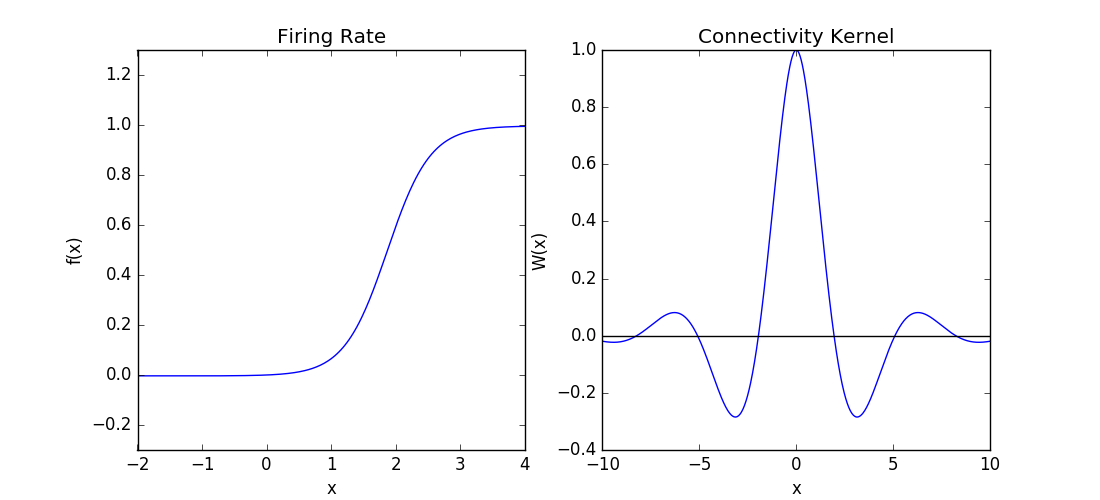
\includegraphics[width=1\textwidth]{Figures/1D_fRate_ker_nystrom.png}
	\end{center}
	\caption{Firing rate function \ref{eqn:1d_firing_rate} and Connectivity Kernel function \ref{eqn:1d_kernel}, for the case where $b = 0.4$, $\mu = 3$, $\theta = 5.6$}
	\label{fig:fRate_ker_nystrom}
\end{figure}

The special choice of the functions \ref{eqn:1d_kernel} and \ref{eqn:1d_firing_rate} were taken as in the Rankin-Avitabile paper \cite{rankin2014continuation}, where, for this particular choice of functions they show the existence of localised bump solutions as the steepness parameter $\mu$ is varied. However, bumps solutions have been shown to exist for different choices of $W$ and $f$, as well as different parameters. In particular, \cite{LaingCarloR.2002MBia} shows the existence of bump solutions for a different choice of $f$ and varying threshold parameter $\theta$.
 
The discretization of eq. \ref{eqn:nf_1dmodel} is carried out in the same way as seen in section \ref{subsec: Nystrom}. First we define the domain $\Omega_h=[-L, L] \subset \mathbb{R}$. Introduce a numerical quadrature scheme to approximate the integral on the right hand side of \ref{eqn:nf_1dmodel} by defining $N$ quadrature points $\{y_j\}_{j=0}^{N-1}$, such that
\begin{equation}
\dot{u}(x, t) \approx -u(x, t) + \sum_{j=0}^{N-1} W(x, y_j)f(u(y_j, t))\rho_j, \hspace{3mm} x \in \mathbb{R},
\end{equation}
where $\rho_j$ are the quadrature weights.

We then discretize the domain $\Omega_h$ by introducing a set of $N$ equally spaced points $\{x_i\}_{i=0}^{N-1}$, such that $x_i = -L + ih, \hspace{3mm} i = 0,...,N-1$ where $h$ is the distance between points. Pick $\{x_i\}$ and $\{y_j\}$ to be coincident, so that we get the fully discretized equation
\begin{equation}
\dot{u}(x_i, t) \approx -u(x_i, t) + \sum_{j=0}^{N-1} W(x_i, x_j)f(u(x_j, t))\rho_j, \hspace{3mm} x_i, y_j \in \Omega_h.
\end{equation}
It is convenient to represent this equation as a time-dependant Matrix-Vector equation:
\begin{equation}\label{eqn:nf_1d_matrix-vector}
\dot{\textbf{u}}(t) = -\textbf{u}(t) + \textbf{W} \hspace{1mm} \textbf{f}(\textbf{u}(t)), \hspace{3mm} \textbf{W} \in \mathbb{R}^{N\times N}, \textbf{u} \in \mathbb{R}^N
\end{equation}
where $\textbf{W}_{i,j} = W(x_i, x_j)\rho_j, \hspace{3mm}  \textbf{f}(\textbf{u}(t)) = f(u(x_i, t)) \hspace{3mm} \forall i,j$. The matrix $\textbf{W}$ is known as the synaptic connectivity matrix and holds information about the influence between neighbouring neurons $x_i$ and $x_j$.

Now that we have a time dependant ordinary differential equation we can find localised (bump) solutions by evolving the equation forward in time using an initial guess in the form of a bell-shaped function. For this we used a fourth-order Runge-Kutta (RK4) scheme (See \cite{heath2002scientific} section 9.6.2). In this work we use the Runge-Kutta4 algorithm provided by \texttt{scipy.integrate.ode} package.  

\subsection{Results}\label{subsec:1Dnystrom_results}

We now present some results of the numerical computations of eqn.\ref{eqn:nf_1d_matrix-vector} similar to those in \cite{rankin2014continuation}.

We are interested in localised solutions of \ref{eqn:nf_1d_matrix-vector} in the form of bump solutions. It has been shown that this solutions are generic and form families that follow a snake-like bifurcation as the parameter $\mu$ (firing threshold) is varied \cite{rankin2014continuation}.

As defined in \cite{LaingCarloR.2002MBia}, a stationary solution is an N-bump solution if its region of excitation consists of exactly N disjoint, finite connected intervals. A region of excitation is the set
\begin{equation}
	R(u) = \{x | u(x)>\mu/\theta \}.
\end{equation}
In other words, an $N$-bump solution crosses the threshold value $\mu/\theta$ $N$ times.

For convenience we set $b=0.4$ and $\theta = 3.5$. At these values, \cite{rankin2014continuation} has shown that the problem \ref{eqn:nf_1dmodel} with \ref{eqn:1d_kernel} - \ref{eqn:1d_firing_rate}, undergoes a series of localised bump solutions with different spatial extent that coexist and are stable when $\mu \in [3,4]$. The number of bumps in the solution depends on the initial profile used for the time stepping. Usually one starts with a bell-shaped initial condition. The wider the shape, the more bumps there are in the stationary solution.

In this case, we start time simulations with the initial condition given by
\begin{equation}
	u(x,0) = \frac{A_0}{\cosh^2(\alpha x)},
\end{equation}  
where the parameter $\alpha$ allows us to vary the ``kurtosis", and $A_0$ the amplitud of the bell-shaped initial condition $u(x,0)$.

Figure \ref{fig:1d_two_and_three_bumps}(a) shows a localised solution that crosses the threshold $\mu/\theta$ twice. In a similar way, figure \ref{fig:1d_two_and_three_bumps}(a) crosses the threshold twice. By varying the parameters of the initial conditions we can also get a four bump and five bump solutions as the ones in figure \ref{fig:1d_four_and_five_bumps}. This results go in accordance with \cite{rankin2014continuation} figure 1.1, where they show a snaking bifurcation diagram for localised bump solutions when $\mu \in [3,4]$.

\begin{figure}%
	\centering
	\subfloat[Parameters: $\mu=3.5$, $A_0=3$, $\alpha=1/5$]{{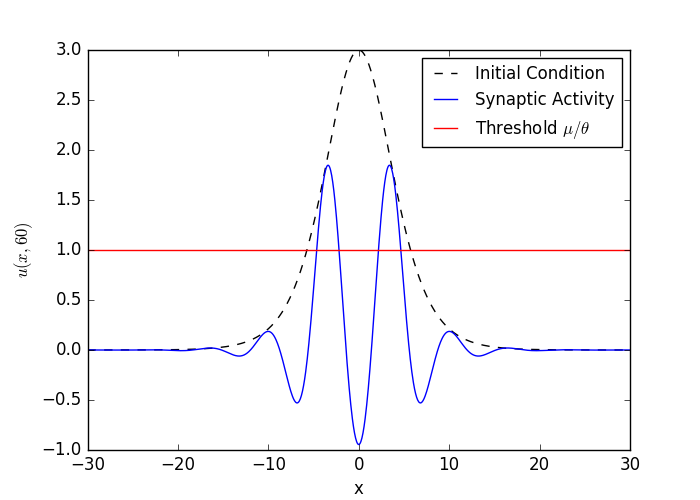
\includegraphics[width=0.46\textwidth]{Figures/1d_2bumps.png} }}%
	\qquad
	\subfloat[Parameters $\mu=3.5$, $A_0=3$, $\alpha=1/10$]{{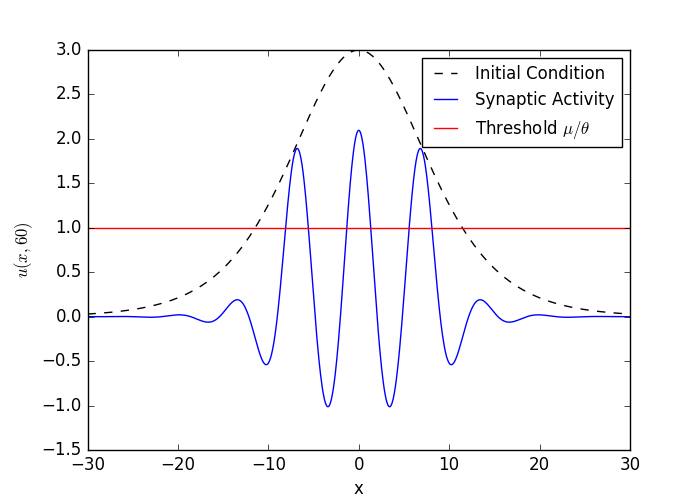
\includegraphics[width=0.46\textwidth]{Figures/1d_3bumps.png} }}%
	\caption{A two bump and three bump solutions, respectively.}%
	\label{fig:1d_two_and_three_bumps}%
\end{figure}

\begin{figure}%
	\centering
	\subfloat[Parameters: $\mu=3.5$, $A_0=9$, $\alpha=1/8$]{{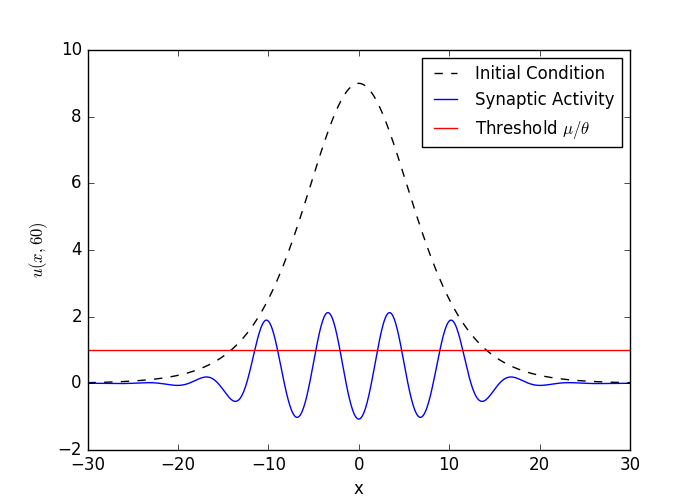
\includegraphics[width=0.46\textwidth]{Figures/1d_4bumps.png} }}%
	\qquad
	\subfloat[Parameters $\mu=3.5$, $A_0=9$, $\alpha=1/10$]{{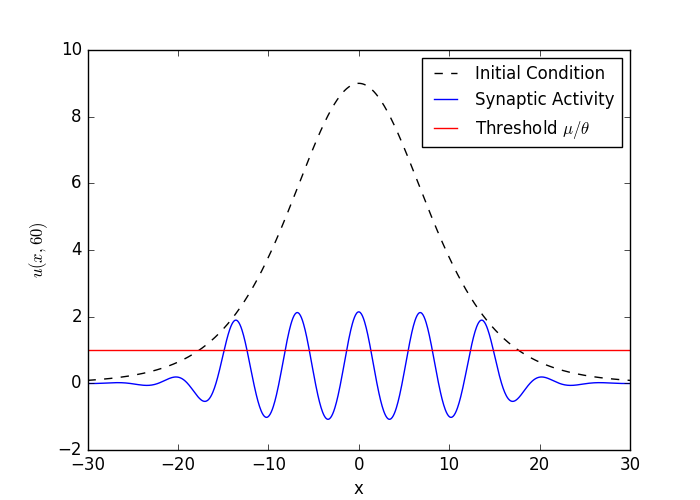
\includegraphics[width=0.46\textwidth]{Figures/1d_5bumps.png} }}%
	\caption{A four bump and five bump solutions, respectively.}%
	\label{fig:1d_four_and_five_bumps}%
\end{figure}

\section{The 2D Model}\label{sec:2d_model}
Now we now proceed with the two dimensional case. Equation \ref{eqn:nf_voltageBased}, for the case $d=2$ is written as
\begin{equation} \label{eqn:2d_nf_nystrom}
	\frac{\partial u(\mathbf{r},t)}{\partial t} = - u(\mathbf{r},t) +
	\int_{D} W(\mathbf{r},\mathbf{r'})f(u(\mathbf{r'},t))
	d\mathbf{r'} + I_{ext}(\mathbf{r},t), \hspace{3mm} \mathbf{r} \in \mathbb{R}^2, \hspace{3mm} D \subset \mathbb{R}^2,
\end{equation}
where, as usual, $W$ denotes the synaptic connectivity kernel and $f$ the firing rate function.

As mentioned earlier, the interpretation of this model is that $u(\mathbf{r},t)$ is the average voltage of a group of neurons positioned at $\mathbf{r} = (x,y)$ in a cortex. The interaction of neurons is mediated by the synaptic connectivity function $W$ and is measured with the Euclidian distance as $W(\|\mathbf{r}-\mathbf{r'}\|_2)$. We make use of Nystr\"om method with a Gaussian Quadrature rule to find bump solutions in a two dimensional region $D \subset \mathbb{R}^2$.

If we write eq. \ref{eqn:2d_nf_nystrom} using an integral operator as the one defined in \ref{eqn:integral_operator}, we get
\begin{equation}\label{eqn:2d_nf_nystrom_integoperator}
\frac{\partial u(\mathbf{r},t)}{\partial t} = I(\mathbf{r},t)- u(\mathbf{r},t) +
\mathcal{K}(u(\mathbf{r},t)),
\end{equation}
here, $\mathcal{K}$ is defined as
\begin{equation}\label{eqn:2d_integoperator}
	\mathcal{K}(u(\mathbf{r},t)) = \int_{D} W(\|\mathbf{r}-\mathbf{r'}\|_2)f(u(\mathbf{r'},t))
	d\mathbf{r'}.
\end{equation}
We let the two dimensional connectivity kernel be
\begin{equation}\label{eqn:2d_kernel}
	W(\mathbf{r},\mathbf{r'}) = e^{-b\|\mathbf{r}-\mathbf{r'}\|}
	\left(b \space \sin(\|\mathbf{r}-\mathbf{r'}\|) + \cos(\|\mathbf{r}-\mathbf{r'}\|)\right),
\end{equation}
with $b=0.4$ controlling the decay of the oscillating behaviour of $W$. And the firing rate function as 
\begin{equation}\label{eqn:2d_firing_rate}
f(u) = \frac{1}{1+e^{-\mu u + \theta}} -\frac{1}{1+e^\theta},
\end{equation}
with $\mu$ controlling the slope of the sigmoidal firing rate and $\mu/\theta$ is the threshold value. A plot of \ref{eqn:2d_kernel} in two dimensions is shown in figure \ref{fig:2d_kernel}. A plot of \ref{eqn:2d_firing_rate} is the same as in the 1D case and can be seen in figure \ref{fig:fRate_ker_nystrom}.

\begin{figure}
	\begin{center}
		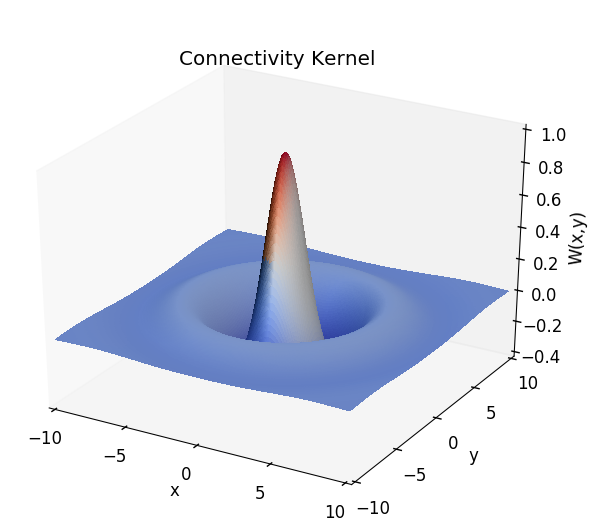
\includegraphics[width=0.6\textwidth]{Figures/2d_kernel.png}
	\end{center}
	\caption{2D connectivity kernel \ref{eqn:2d_kernel}, for $b = 0.4$}
	\label{fig:2d_kernel}
\end{figure}

\subsection{Nystr\"om Discretization in 2D}\label{subsec:2d_nystrom}
Nystr\"om method in two dimensions follows in much the same way as in the one dimensional case presented in section \ref{subsec: Nystrom} with some minor modifications.

First we introduce a two-dimensional numerical quadrature scheme for a generic function $g: \mathbb{R}^2 \rightarrow \mathbb{R}$ as
\begin{equation}
	\iint_D f(x,y) dxdy \approx \sum_{k=0}^{n} \sum_{l=0}^{m} f(x_k, y_l)\rho_k\rho_l,
\end{equation}
where $x_k , y_l$ are the quadrature \textit{nodes} and $\rho_k\rho_l$ are quadrature \textit{weights}, with $n,m \geq 0$. Now we can get an approximation of the integral operator \ref{eqn:2d_integoperator} as
\begin{equation}
	\mathcal{K}_h(u(\mathbf{r},t)) \approx \sum_{k=0}^{n} \sum_{l=0}^{m} W(\| \mathbf{r} - (x_k, y_l) \|)f(u_{kl}(t))\rho_k \rho_l,
\end{equation} 
where we have let $u_{kl}(t) = u((x_k, y_l),t)$ for convenience.

Now, by using the same set of points $\{(x_k, y_l)\}$ for the collocation grid as for the quadrature rule, we can write the fully discretized version of eq.\ref{eqn:2d_nf_nystrom_integoperator} as
\begin{equation} \label{eqn:2d_fully_discrete}
\dot{u}_{ij}(t) \approx - u_{ij}(t) + \sum_{k=0}^{n} \sum_{l=0}^{m} W(\| (x_i, y_j) - (x_k, y_l) \|)f(u_{kl}(t))\rho_k \rho_l.
\end{equation}

\subsection{Computational Implementation}\label{subsec:2d_comp_implementation}
We will be using Nystr\"om method with a Gaussian quadrature rule on a rectangular region $\Omega = [-L, L] \times [-L, L]$ in a similar way as Lima and Buckwar do on their paper \cite{lima2015numerical}, section 2.1.2.

We start by discretizing the domain $\Omega$. Let $\{x_i\}$ be a uniform set of points such that $x_i = -L + ih$, $i=0,...,n-1$, where $h$ is the distance between points. In each subinterval $[x_i, x_{i+1}]$ introduce $q$ Gaussian (interior) points by defining
\begin{equation}\label{eqn:2d_gauss_interior}
	\varphi_i^s = \varphi^s(x_i) = x_i + \frac{h}{2}(1 + \xi_s), \hspace{3mm} s = 1,...,q,
\end{equation}
where $\xi_s$, as in Gaussian quadrature, are the roots of the Legendre polynomial of degree $q$. Now we have a new uniform set of interior points  $\{\varphi_i^{s}\}$ for $i=0,...,n-1,$ and $s=1,...,q$. By taking a cross-product of $\{\varphi_i^s\}$ with itself we get our set of grid points $\Omega_h = \{(\varphi_i^s, \varphi_j^{s'})\}$, such that $i,j = 0,...,n-1; s,s' = 1,...,q$. Note that the set $\Omega_h$ contains $N^2$ points, where $N=(n-1)q$. A python function for assembling the grid $\Omega_h$ is included in listing \ref{lst:2d_points_grid}.\\
\begin{listing}[H]
	\begin{center}
		\begin{minted}{python}
def assembleGrid(x_pts, g_pts):
	"""
	Function: assembleGrid
	----------------------
	Receives:
		x_pts: set of equally spaced points
		g_pts: set of Gauss interior points in [-1,1]
	Returns:
		grid:  array of interior points with shape (N^2, 2), 
			where N = (len(x_pts)-1)*len(g_pts)
	"""
	n = len(x_pts); q = len(g_pts)
	hx = x_pts[1] - x_pts[0]; 
	grid = []
	for i in range(n-1):
		x = x_pts[i]
		for s in range(q):
			int_x = x + (hx/2)*(1+g_pts[s])
			for j in range(n-1):
				y = x_pts[j]
				for t in range(q):
					int_y = y + (hx/2)*(1+g_pts[t])
					new_pt = [int_x, int_y]
					grid.append(new_pt)
	return grid
		\end{minted}	
	\end{center}
	\caption{python function for assembling the grid $\Omega_h$ with Gaussian interior points as defined in \ref{eqn:2d_gauss_interior}}
	\label{lst:2d_points_grid}.
\end{listing} 
The discretized equation \ref{eqn:2d_fully_discrete} posed on $\Omega_h$ then becomes
\begin{equation}\label{eqn:2s_nf_gquad}
	\dot{u}_{ij}(t) \approx - u_{ij}(t) + \sum_{k=0}^{n} \sum_{l=0}^{m} W(\| (\varphi_i^s, \varphi_j^{s'}) - (\varphi_k^s, \varphi_l^{s'}) \|)f(u_{kl}(t))\tilde{\rho_k} \tilde{\rho_l},
\end{equation}
where now, $ u_{ij}(t) = u((\varphi_i^s, \varphi_j^{s'}),t)$ with $\varphi_i^s$ being Gaussian interior \textit{nodes} given by eq. \ref{eqn:2d_gauss_interior}, and $\tilde{\rho_k} = \frac{h}{2}\rho_k$ with $\rho_k$ the standard weights of a Gaussian quadrature formula with nodes on $[-1,1]$.

As already mentioned, it is convenient to write equation \ref{eqn:2s_nf_gquad} as a matrix-vector equation using a synaptic matrix $\mathbf{W}$. Then we get
\begin{equation}\label{eqn:2d_mat_vec}
	\dot{\mathbf{u}}(t) = -\mathbf{u}(t) + \mathbf{W} \hspace{1mm} \textbf{f}(\mathbf{u}(t)), \hspace{3mm} \mathbf{W} \in \mathbb{R}^{N^2 \times N^2}, \mathbf{u} \in \mathbb{R}^{N^2},
\end{equation}
where $N = (n-1)q$, with 

\begin{subequations}
	\begin{align}
	\mathbf{W}_{i,j} &= W(\| (\vec{\varphi}_i - \vec{\varphi}_j) \|)\tilde{\rho_i} \tilde{\rho_j}, 
	\hspace{3mm} \textnormal{and}\\
	\textbf{f}(\mathbf{u}_i(t)) &= f(u(\vec{\varphi}_i,t))
	\hspace{3mm} \forall \hspace{1mm} i,j = 0,...,N,
	\end{align}
\end{subequations}
here we have let $\vec{\varphi} \in \Omega_h$ be a point inside the grid $\Omega_h$, such that $\vec{\varphi}_i = (\varphi_k^s, \varphi_l^{s'})$ for some $k,l,s,s'$. 

To assemble the synaptic matrix $\mathbf{W}$ it is required to iterate through each grid point twice. Hence, $O(N^4)$ operations are needed, where $N=(n-1)q$ (Recall that the grid is comprised of $N^2$ points). We can halve time it takes to assemble the matrix by using the symmetry of the connectivity kernel function, that is $W(\|\textbf{r}-\textbf{r'}\|_2)=W(\|\textbf{r'}-\textbf{r}\|_2)$, and by exploiting the efficiency of python's \texttt{numpy} package. In other words, we can compute the values of $\mathbf{W}$ just for the upper triangular part, and then devise a strategy to efficiently copy the upper triangular values to the lower triangular part of $\mathbf{W}$. After that we multiply times a vector that contains the values of the quadrature weights $\rho_k\rho_l, \hspace{3mm} k,l=1,...,q$. An example of a python function that assembles the synaptic matrix $\mathbf{W}$ is given in listing \ref{lst:2d_synap_mat}.

Once assembled the synaptic matrix $\mathbf{W}$, a right-hand side evaluation of the discretized equation \ref{eqn:2d_mat_vec} consists of a matrix vector multiplication, as in listing \ref{lst:2d_computeF}. With the function to compute the right hand side of eq. \ref{eqn:2d_mat_vec} we can proceed with the time stepping using RK4 algorithm to find localised bump solutions. In this work we use the Runge-Kutta4 algorithm provided by \texttt{scipy.integrate.ode} package. Information about RK4 algorithms see \cite{heath2002scientific} section 9.6.2.
\begin{listing}[H]
		\begin{minted}{python}
def assembleSynapticMatrix(grid, g_wgts, kernel, h, n, q):
	"""
	Function: assembleSynapticMatrix
	--------------------------------
	Receives:
		grid: array of interior points.
		g_wgts: Gauss weights on the [-1,1] interval.
		kernel: Synaptic connectivity kernel function.
		h: spacing between points.
		n: number of points in the x-axis.
		q: number of interior gauss nodes used for the grid.
	Returns:
		Synaptic Matrix W of shape (N_sq,N_sq) where N_sq is the length
		of the grid. i.e. N_sq = ( (n-1)*q )^2
	"""
	wgts_h = (h/2)*g_wgts # Scale weights
	# Weights vector:
	wgts = numpy.tile(wgts_h, n-1)
	wgts = numpy.outer(wgts.T, wgts)
	wgts = wgts.flatten()
	
	N_sq = len(grid); W = numpy.zeros( (N_sq, N_sq) )
	# Compute only the upper triangular part
	for i in range(0, N_sq):
		x_pt=grid[i]
		for j in range(i, N_sq):
			y_pt = grid[j]
			x, y = x_pt-y_pt
			W[i,j] = kernel(x, y)
	
	# Copy upper triangular part to lower triangular part
	i_lower = numpy.tril_indices(N_sq, -1)
	W[i_lower] = W.T[i_lower]
	
	W *= wgts # Multiply times the weights (pointwise multiplication)
	return W
		\end{minted}	
	\caption{python function for assembling the synaptic matrix $\textbf{W}$}
	\label{lst:2d_synap_mat}
\end{listing}
\begin{listing}[H]
	\begin{center}
		\begin{minted}{python}
def computeF(u, f_rate, W):
	"""
	Function: computeF
	----------------------
	One evaluation of the right hand side.
	Receives:
		u: current state vector to evaluate at
		W: pre-built synaptic matrix
		f_rate: callable firing rate function
	"""
	f_u = f_rate(u) # Evaluate firing rate function at the vector u
	return -u + W.dot(f_u)
		\end{minted}	
	\end{center}
	\caption{Pseudocode for evaluating the right hand side of equation \ref{eqn:2d_mat_vec}}
	\label{lst:2d_computeF}
\end{listing}

\subsection{Numerical Experiments} \label{subsec:2d_tests}
In this part we present the results of some numerical tests that were carried out to measure the error of the method as the mesh is refined. The cases were drawn from the Lima and Buckwar paper \cite{lima2015numerical}, section 3. Although this cases have no biological relevance, they provide us with a benchmark to test the implemented algorithm.

\textit{Example 1.} For this example, the connectivity kernel is given by
\begin{equation}\label{eqn:2d_test1_W}
W(\textbf{r},\textbf{r'}) = W(x_1,y_1,x_2,y_2) = \exp\left(-\lambda (x_1- y_1)^2 - \lambda (x_2-y_2)^2\right), \hspace{3mm} \lambda \in \mathbb{R}^+.
\end{equation}
The firing rate function by
\begin{equation}\label{eqn:2d_test1_frate}
	f(\mathbf{u}) = \tanh(\sigma \mathbf{u}), \hspace{3mm} \sigma \in \mathbb{R}^+, \mathbf{u} \in \mathbb{R}^2,
\end{equation}
and we incorporate en external input $I_{ext}$ given by
\begin{equation}\label{eqn:2d_test1_Iext}
	I_{ext}(x,y,t) = -\tanh\left( \sigma \exp \left( -\frac{t}{c}\right)\right) b(x_1,y_1;\lambda),
\end{equation}
where
\begin{equation}\label{eqn:2d_test1_b}
\begin{split}
	b(x1,y1;\lambda) &= \int_{-1}^{1} \int_{-1}^{1} W(x_1,y_1,x_2,y_2)dy_1dy_2\\
	&=\frac{\pi}{4\lambda}\left( \textnormal{Erf}(\sqrt{\lambda}(1-x_1)) + \textnormal{Erf}(\sqrt{\lambda}(1+x_1))\right) \left( \textnormal{Erf}(\sqrt{\lambda}(1-x_2)) + \textnormal{Erf}(\sqrt{\lambda}(1+x_2))\right),
\end{split}
\end{equation}
where Erf represents the Gaussian error function.

For this case, the exact solution is
\begin{equation}
	u(\textbf{r}, t) = \exp \left( - \frac{t}{c}\right).
\end{equation}

The objective is to measure the error as the mesh grid is refined. We begin with a mesh comprised by $n=2$ points in the $x$-axis and $q=2$ Gaussian nodes, then the grid will contain $N^2$ points where $N = (n-1)q$, and we keep refining the grid measuring the true solution at the final time against the computed solution at the final time in the infinity norm, in the sense that
\begin{equation}\label{eqn:2d_ex1_errormeasure}
	e_T(h) = \| u(\mathbf{r}, T) - u_h(\mathbf{r}, T)\|_{\infty}, \hspace{3mm} \mathbf{r}\in\mathbb{R}^2
\end{equation}
is the error measured at the final time $T$ that depends on the spacing between points $h$. We start the time stepping with an initial condition given by 
\begin{equation}
u(\textbf{r}, 0) \equiv 1,
\end{equation}
from the initial time $t=0$ to the final time $T=1$ with step size of $h_t=0.1$.

As is well known, a Gaussian quadrature with precision rule $q$ has an integration error of order $h^{2q}$. Therefore, for a precision rule of $q=2$, we expect a behaviour of the type
\begin{equation}
e_T = \| u(\mathbf{r}, T) - u_h(\mathbf{r}, T)\|_{\infty} = O(h^4)
\hspace{3mm} \textnormal{as}\hspace{3mm} h \rightarrow 0.
\end{equation}
where $h$ is the spacing between points. See \cite{lima2015numerical} section 2.1.2, theorem 2.4.

Table \ref{table:2dErrors_test1_q2} contains the measure of the errors $e_T(h)$ for more refined mesh grids. First column $n$ are the number of points in the $x$-axis, second column $N^2$ are the total number of points in the grid, third column $h$ is the spacing between points, fourth column $e_T(h)$ is the error measure \ref{eqn:2d_ex1_errormeasure}. Figure \ref{fig:2dErrors_test1_q2} shows the error measures \ref{eqn:2d_ex1_errormeasure} (blue dots) on top of an actual $O(h^4)$ curve (red line), providing numerical evidence of an $O(h^4)$ behaviour.
\begin{table}[H]
	\centering
\begin{tabular}{|c|c|c|c|}
	\hline
	$n$&$N^2$&$h$&$e_T(h)$\\
	\hline
	2&4&2.0&0.0023\\
	3&16&1.0&0.0013\\
	4&36&0.667&0.0002\\
	5&64&0.5&9.02e-05\\
	6&100&0.4&3.68e-05\\
	7&144&0.333&1.77e-05\\
	8&196&0.286&9.58e-06\\
	9&256&0.25&5.62e-06\\
	10&324&0.222&3.50e-06\\
	\hline
\end{tabular}
\caption{Table containing the errors of \textit{example 1} for a more refined mesh grid using a two point $q=2$ precision rule. Parameters were set as $\lambda=1$, $\sigma=1$, $c=1$.}
\label{table:2dErrors_test1_q2}
\end{table}

\begin{figure}[H]
	\begin{center}
		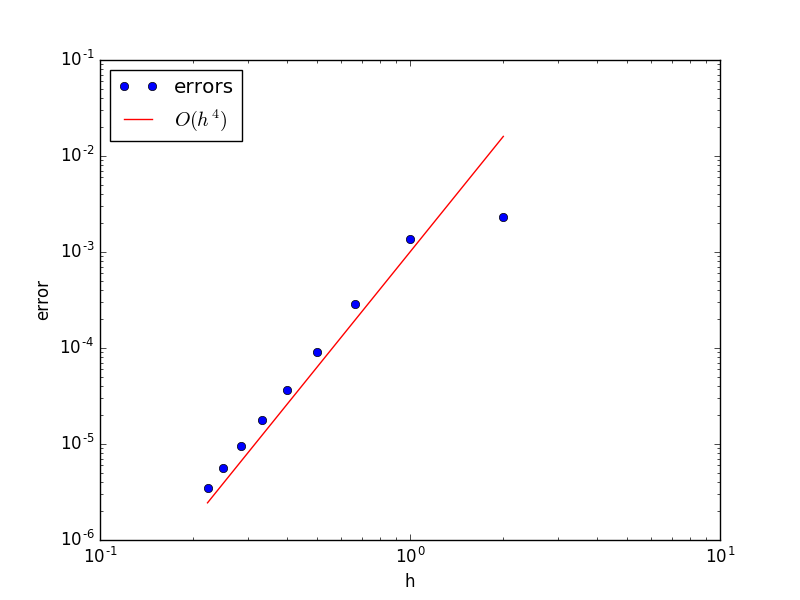
\includegraphics[width=0.7\textwidth]{Figures/2dRectTest1_q=2.png}
	\end{center}
	\caption{Plot of errors v.s. an actual $h^4$ curve, for \textit{example 1} using a two precision rule $q=2$, on a log-log scale. Mesh refinement $h$ on the $x$-axis, error measures on the $y$-axis. Parameters were set as $\lambda=1$, $\sigma=1$, $c=1$.}
	\label{fig:2dErrors_test1_q2}
\end{figure}

Continuing with the same \textit{example 1} but now using a four precision rule $q=4$, then we expect an $O(h^8)$ behaviour, in the sense that
\begin{equation}\label{eqn:2d_test1_escrom}
e_T = \| u(\mathbf{r}, T) - u_h(\mathbf{r}, T)\|_{\infty} = O(h^8)
\hspace{3mm} \textnormal{as}\hspace{3mm} h \rightarrow 0,
\end{equation}
where $h$ is the spacing between points. See \cite{lima2015numerical} section 2.1.2, theorem 2.4.

Table \ref{table:2dErrors_test1_q4} contains the measure of the errors $e_T(h)$ \ref{eqn:2d_ex1_errormeasure} for more refined mesh grids. Figure \ref{fig:2dErrors_test1_q4} shows the error measures \ref{eqn:2d_ex1_errormeasure} (blue dots) on top of an actual $O(h^8)$ curve (red line), providing numerical evidence of an $O(h^8)$ behaviour.

\begin{table}[H]
	\centering
	\begin{tabular}{|c|c|c|c|}
		\hline
		$n$&$N^2$&$h$&$e_T(h)$\\
		\hline
		2&16&2.0&0.0001\\
		3&64&1.0&5.86e-07\\
		4&144&0.667&1.06e-08\\
		5&256&0.5&8.01e-10\\
		6&400&0.4&4.89e-10\\
		\hline
	\end{tabular}
	\caption{Table containing the errors of \textit{example 1} for a more refined mesh grid using a four point $q=4$ precision rule. Parameters were set as $\lambda=1$, $\sigma=1$, $c=1$.}
	\label{table:2dErrors_test1_q4}
\end{table}

\begin{figure}[H]
	\begin{center}
		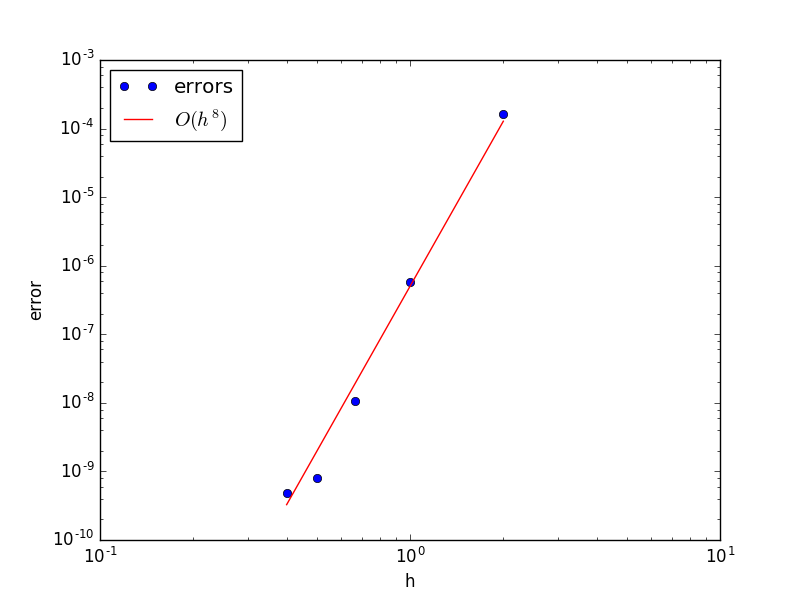
\includegraphics[width=0.7\textwidth]{Figures/2dRectTest1_q=4.png}
	\end{center}
	\caption{Plot of errors v.s. an actual $h^8$ curve, for \textit{example 1} using a four precision rule $q=4$, on a log-log scale. Mesh refinement $h$ on the $x$-axis, error measures on the $y$-axis. Parameters were set as $\lambda=1$, $\sigma=1$, $c=1$.}
	\label{fig:2dErrors_test1_q4}
\end{figure}

\textit{Example 2}. For the second example we take the same equation \ref{eqn:2d_test1_W} for $W$, and \ref{eqn:2d_test1_frate} for the firing rate $f$. We set the external input as
\begin{equation}
	I_{ext} = c + t -\tanh(\sigma t)b(x,y;\lambda),
\end{equation}
with $b(x,y;\lambda)$ the same as in eq. \ref{eqn:2d_test1_b}. We will carry the same analysis as in \textit{example 1} except that we are now going to vary the parameters $\lambda, \sigma, c$. We will stick with a four precision rule $q=4$, meaning that we expect an $O(h^8)$ behaviour for the errors, as in eq. \ref{eqn:2d_test1_escrom}. Table \ref{table:2dErrors_test2_q4} contains the measure of the errors $e_T(h)$ \ref{eqn:2d_ex1_errormeasure} for more refined mesh grids, for the three cases. Case 1 is when: $\lambda=1$, $\sigma=1$, $c=1$, for case 2 we set: $\lambda=1$, $\sigma=5$, $c=1$, and in case 3: $\lambda=5$, $\sigma=5$, $c=1$.  Figures \ref{fig:2dErrors_test2_q4_case1}-\ref{fig:2dErrors_test2_q4_case2}-\ref{fig:2dErrors_test2_q4_case3} show the error measures \ref{eqn:2d_ex1_errormeasure} (blue dots) on top of an actual $O(h^8)$ curve (red line), for the three different cases. Notice how the three cases show an $O(h^8)$ behaviour, providing evidence that the algorithm is correct.

\begin{table}[H]
	\centering
	\begin{tabular}{|c|c|c|c||c|c|c|c||c|c|c|c||}
		\hline
		\multicolumn{4}{|c||}{Case 1}&
		\multicolumn{4}{|c||}{Case 2}&
		\multicolumn{4}{|c||}{Case 3}\\
		\multicolumn{4}{|c||}{$\lambda=1$, $\sigma=1$, $c=1$}&
		\multicolumn{4}{|c||}{$\lambda=1$, $\sigma=5$, $c=1$}&
		\multicolumn{4}{|c||}{$\lambda=5$, $\sigma=5$, $c=1$}\\
		%\hline
		$n$&$N^2$&$h$&$e_T(h)$&
		$n$&$N^2$&$h$&$e_T(h)$&
		$n$&$N^2$&$h$&$e_T(h)$\\
		\hline \hline
		2&16&2.0&0.0001&
		2&16&2.0&0.0002&
		2&16&2.0&0.0283\\
		3&64&1.0&6.37e-07&
		3&64&1.0&1.14e-06&
		3&64&1.0&0.0001\\
		4&144&0.667&1.03e-08&
		4&144&0.667&1.71e-08&
		4&144&0.667&1.67e-05\\
		5&256&0.5&9.57e-10&
		5&256&0.5&1.65e-09&
		5&256&0.5&7.71e-07\\
		6&400&0.4&1.50e-10&
		6&400&0.4&2.45e-10&
		6&400&0.4&5.12e-08\\
		7&576&0.333&3.37e-11&
		7&576&0.333&5.74e-11&
		7&576&0.333&8.78e-09\\
		8&784&0.286&9.58e-12&
		8&784&0.286&1.59e-11&
		8&784&0.286&2.51e-09\\
		9&1024&0.25&3.24e-12&
		9&1024&0.25&5.53e-12&
		9&1024&0.25&8.04e-10\\
		10&1296&0.222&1.25e-12&
		10&1296&0.222&2.10e-12&
		10&1296&0.222&2.97e-10\\
		\hline
	\end{tabular}
	\caption{Table containing the errors of \textit{example 2} for a more refined mesh grid using a four point $q=4$ precision rule, for three different cases of parameter values. Case1: $\lambda=1$, $\sigma=1$, $c=1$, Case2: $\lambda=1$, $\sigma=5$, $c=1$, Case3: $\lambda=5$, $\sigma=5$, $c=1$.}
	\label{table:2dErrors_test2_q4}
\end{table}

\begin{figure}[H]
	\begin{center}
		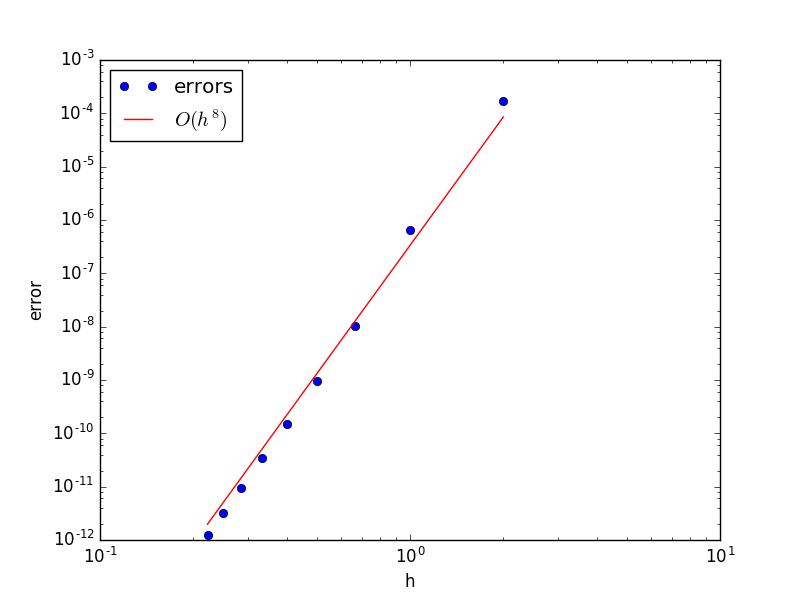
\includegraphics[width=0.7\textwidth]{Figures/2dRectTest2_q=4_case1.png}
	\end{center}
	\caption{Plot of errors v.s. an actual $h^8$ curve, for \textit{example 2} using a four precision rule $q=4$, on a log-log scale. Mesh refinement $h$ on the $x$-axis, error measures on the $y$-axis. Parameters were set as $\lambda=1$, $\sigma=1$, $c=1$.}
	\label{fig:2dErrors_test2_q4_case1}
\end{figure}

\begin{figure}[H]
	\begin{center}
		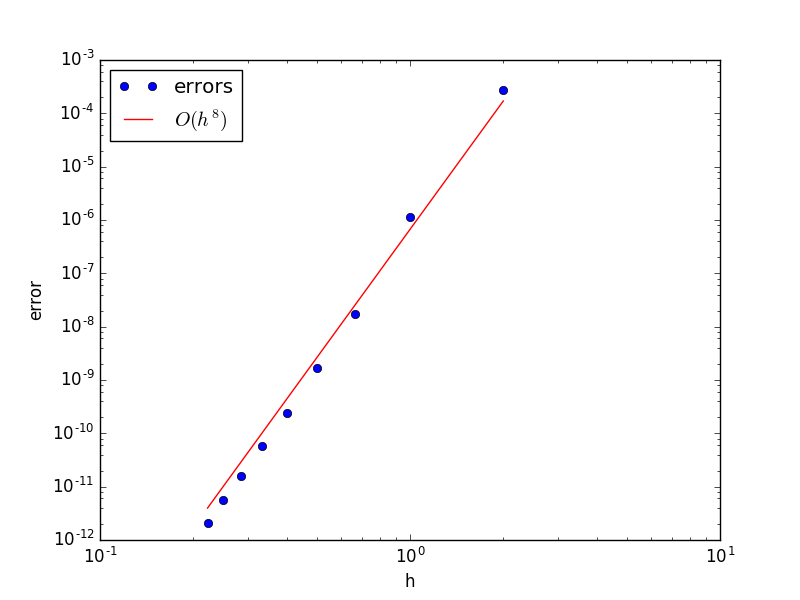
\includegraphics[width=0.7\textwidth]{Figures/2dRectTest2_q=4_case2.png}
	\end{center}
	\caption{Plot of errors v.s. an actual $h^8$ curve, for \textit{example 2} using a four precision rule $q=4$, on a log-log scale. Mesh refinement $h$ on the $x$-axis, error measures on the $y$-axis. Parameters were set as $\lambda=1$, $\sigma=5$, $c=1$.}
	\label{fig:2dErrors_test2_q4_case2}
\end{figure}

\begin{figure}[H]
	\begin{center}
		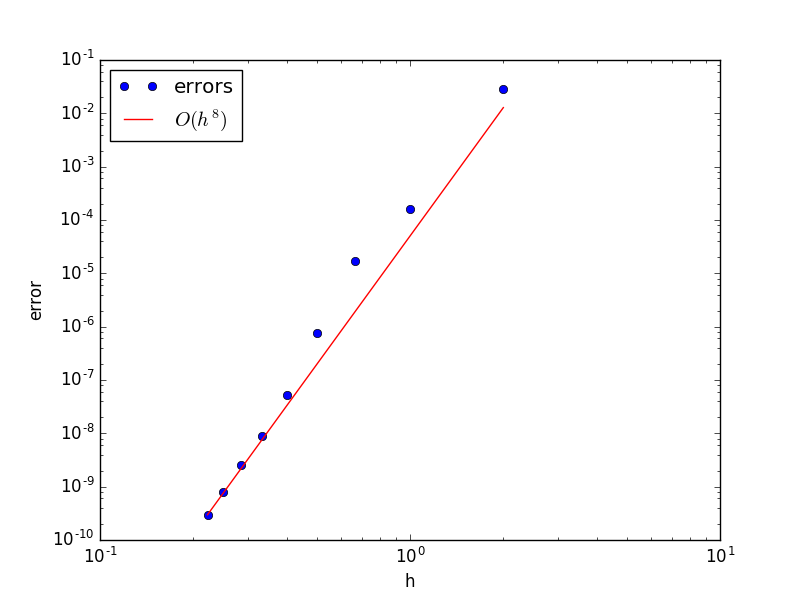
\includegraphics[width=0.7\textwidth]{Figures/2dRectTest2_q=4_case3.png}
	\end{center}
	\caption{Plot of errors v.s. an actual $h^8$ curve, for \textit{example 2} using a four precision rule $q=4$, on a log-log scale. Mesh refinement $h$ on the $x$-axis, error measures on the $y$-axis. Parameters were set as $\lambda=5$, $\sigma=5$, $c=1$.}
	\label{fig:2dErrors_test2_q4_case3}
\end{figure}

\subsection{Results} \label{subsec:2d_results}
For the Neural Field equation in two dimensions, different types of spatially localised two-dimensional states have been found including radially symmetric solutions \cite{laing2003pde,LaingCarloR.2002MBia}, breathing and traveling states \cite{coombes2014spots,owen2007bumps}, rings \cite{coombes2012interface,owen2007bumps} and hexagonal patches\cite{laing2003pde,rankin2014continuation}. In this section we implement the Nystr\"om method developed in section \ref{subsec:2d_nystrom} to find some patterns of activity in the form of hexagonal patches and radially-symmetric spots, as the ones presented in \cite{rankin2014continuation}, page 4. We see how different combinations of initial conditions and control parameters lead to different patterns.

As in \cite{rankin2014continuation}, we fix $b=0.4$ and $\theta=5.6$ in equations \ref{eqn:2d_kernel}-\ref{eqn:2d_firing_rate}, and explore different values for $\mu$ (slope of the sigmoidal firing rate). Time simulations are carried out for $t \in [0,15]$ with a time step size of $h_t = 0.1$. We explore two different initial conditions:
\begin{subequations}
	\begin{align}
		u(\mathbf{r},0) = u(x,y) &= A \exp \left(-\frac{x^2+y^2}{L}\right), \hspace{3mm} \textnormal{and} \label{eqn:2d_initcond1}\\
		u(\mathbf{r},0) = u(x,y) &= A \exp \left(-\frac{x^2+y^2}{L}\right) \left[ \cos(x) + \cos\left( \frac{1}{2}x + \frac{\sqrt{3}}{2}y\right) + \cos\left( -\frac{1}{2}x + \frac{\sqrt{3}}{2}y\right)\right].\label{eqn:2d_initcond2}
	\end{align}
\end{subequations}
on a grid of $n=20$ points on the $x$-axis and $q=3$ interior Gauss points, meaning that the grid is comprised of $N^2 = (n-1)^2q^2 = 3,249$ points.

First we explore a small bump of activity given by the initial condition \ref{eqn:2d_initcond1}. We found different outcomes for varying values of $\mu$. Particularly, we found that: for values $\mu < 3$, the initial bump evolves towards a steady state $u \equiv 0$. When $\mu \in [3,4]$ a radially-symmetric spot solution starts to generate by increasing its height as $\mu \rightarrow 4$, the bump then evolves to a convergent spot with constant height for values of $\mu \in [4,5]$, and it finally diverges towards bump solutions that invade the domain when $\mu > 5$. We display some of this scenarios on figure \ref{fig:2dRect_IC1}, where we plot the time evolution on each column starting with the small bump of activity given by  \ref{eqn:2d_initcond1}, for different values of $\mu$ on each row.

Now we start the time simulations using initial condition \ref{eqn:2d_initcond2} which is a hexagonal pattern. Again, we found different outcomes for varying values of $\mu$. Particularly, we found that: for values $\mu < 2.5$, the initial bump evolves towards a steady state $u \equiv 0$. When $\mu \in [2.5,3]$ the hexagonal pattern converges to a stable symmetric localised state. Then, for values $\mu > 3$ we see a divergence away from the hexagonal pattern to localised bump solutions that invades the entire domain. The bigger the value of $\mu$, the faster the bumps invade the domain. We can see some of this scenarios on figure \ref{fig:2dRect_IC2}, where we plot the time evolution on each column starting with a hexagonal pattern given by  \ref{eqn:2d_initcond2} for different values of $\mu$ on each row.{\tiny }

\begin{figure}[H]
	\begin{center}
	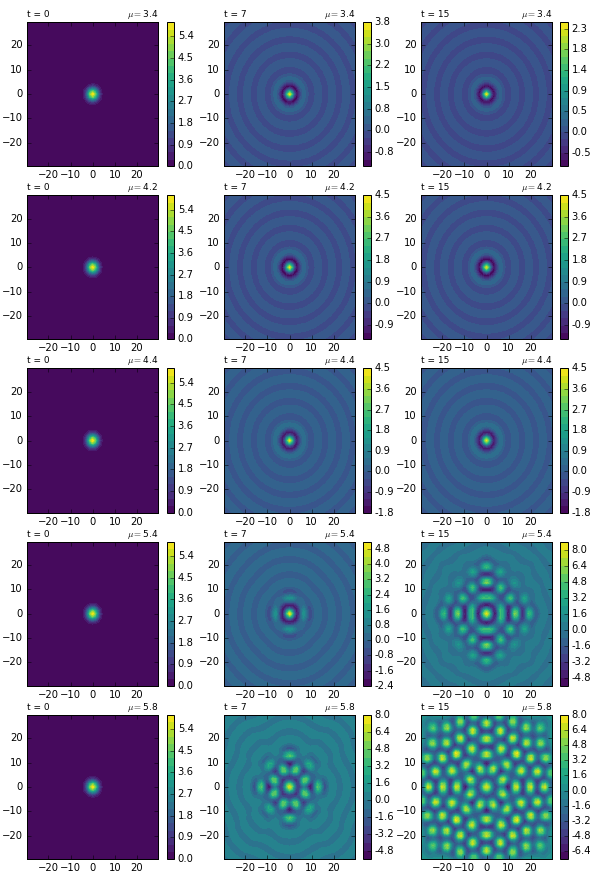
\includegraphics[width=0.8\textwidth]{Figures/2dRect_IC1_3249points.png}
	\end{center}
	\caption{Time simulation of the model \ref{eqn:2d_mat_vec} using \ref{eqn:2d_initcond1} as initial condition with $A = 6$ and $L = 5.77$, with different scenarios of $\mu$ on each row. On the first row $\mu = 3.4$ and displays the radially-symmetric spot with a smaller height. Rows two and three show the convergent spot solution with constant height for values of $\mu = 4.2$ and $\mu = 4.4$ respectively. Finally, on rows four and five we can see the divergence towards invading bump solutions for $\mu=5.4$ and $\mu=5.8$ respectively.}
	\label{fig:2dRect_IC1}
\end{figure}

\begin{figure}[H]
	\begin{center}
		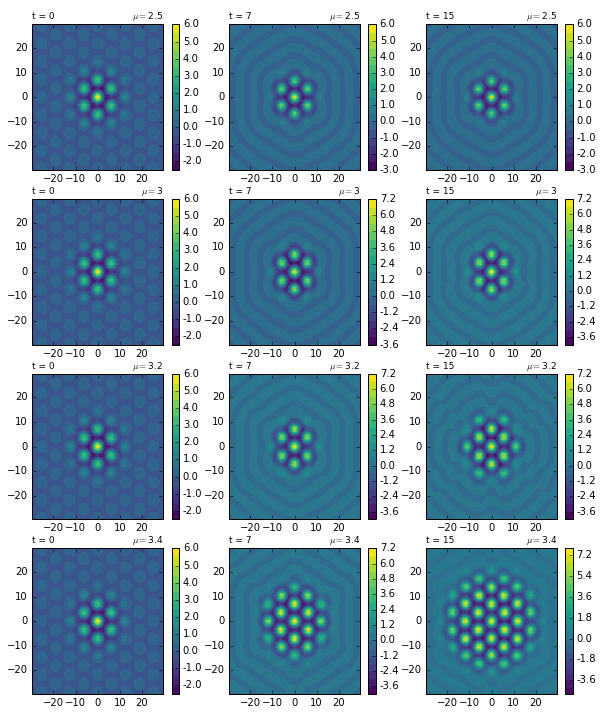
\includegraphics[width=0.8\textwidth]{Figures/2dRect_IC2_3249points.png}
	\end{center}
	\caption{Time simulation of the model \ref{eqn:2d_mat_vec} using a hexagonal pattern given by \ref{eqn:2d_initcond1} as initial condition with $A = 2$ and $L = 100$, with different scenarios of $\mu$ on each row. On the first and second rows we show how the hexagonal pattern converges to a stable symmetric localised state for $\mu = 2.5$ and $\mu = 3$ respectively. Third and forth rows display different rates of divergence to localised bump solutions that ultimately invade the entire domain, for $\mu=3.2$ and $\mu=3.4$ respectively.}
	\label{fig:2dRect_IC2}
\end{figure}

%------------------------------------
\section{The 2D Model on a Triangulated Mesh}
\label{sec:nf_t_domain}
On this section we extend the method developed in section \ref{sec:2d_model} to work on a mesh consisting of triangular elements using Nystr\"om method with a Gaussian quadrature rule.

On section \ref{subsec:gquad_t_elems} we discuss Gaussian quadrature rule for single elements. Then, on section \ref{subsec:GQuad_t_mesh} we extend the quadrature rule for triangulated meshes. After this, on section \ref{subsec:tri nystrom discretize} we use the developed quadrature rule to discretize the equation on a triangulated mesh using Nystr\"om method. On section \ref{subsec:tri_num_experiments} we test the algorithm by studying the error behaviour on pre-built cases where we know the exact solution before hand. Finally, on section \ref{subsec:tri_results}, we validate the method by reproducing the results obtained in section \ref{subsec:2d_results}, as well as in previous studies.


\subsection{Gaussian Quadrature on Triangular Elements}
\label{subsec:gquad_t_elems}
Before solving the neural field equation we explain how Gaussian quadrature is performed over a triangular element.

Let $\kappa$ be a triangular element with vertices given by $(x_i, y_i), i = 1,2,3$ arranged counter-clockwise. As in Figure \ref{fig:tri_elem}.

\begin{figure}[h]
\centering
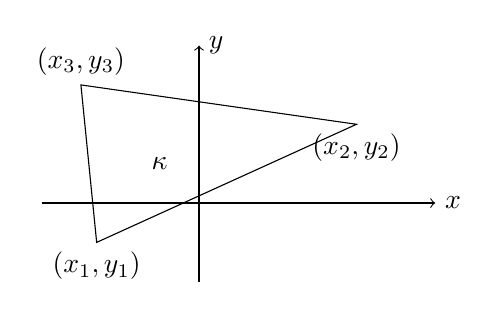
\begin{tikzpicture}
\draw [->] (0,-1) -- (0,2) node[right]{$y$};
\draw [->] (-2,0) -- (3,0) node[right]{$x$}; 
\draw (-1.3,-.5) node[anchor=north]{$(x_1, y_1)$}
-- (2,1) node[anchor=north]{$(x_2, y_2)$}
-- (-1.5,1.5) node[anchor=south]{$(x_3, y_3)$}
-- cycle;
\node at (-0.5,0.5) {$\kappa$};

\end{tikzpicture}
\caption{A triangular element $\kappa$.}
\label{fig:tri_elem}
\end{figure}
We want to evaluate 
\begin{equation}
I = \iint_{\kappa} F(x,y) dxdy.
\end{equation}

The idea is to map the element $\kappa$ to a reference/canonical element $\hat{\kappa}$, as in Figure \ref{fig:tri_map}, and perform integration over $\hat{\kappa}$.

\begin{figure}[h]
	\centering
	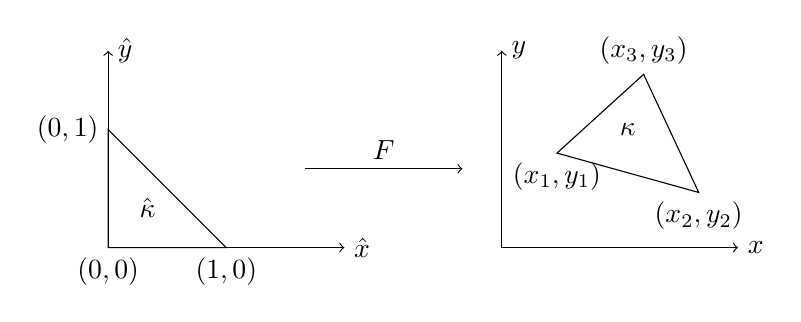
\begin{tikzpicture}
	% center arrow
	\draw [->] (-1.5,0) -- (0.5, 0) node[midway, above]{$F$};
	% Element figure
	\draw [->] (1,-1) -- (1,1.5) node[right]{$y$};
	\draw [->] (1,-1) -- (4,-1) node[right]{$x$}; 
	\draw (3.5,-0.3) node[anchor=north]{$(x_2,y_2)$}
	-- (1.7,0.2) node[anchor=north]{$(x_1,y_1)$}
	-- (2.8,1.2) node[anchor=south]{$(x_3,y_3)$}
	-- cycle;
	\node at (2.6,0.5) {$\kappa$};
	% Canonical element figure
	\draw [->] (-4,-1) -- (-4,1.5) node[right]{$\hat{y}$};
	\draw [->] (-4,-1) -- (-1,-1) node[right]{$\hat{x}$}; 
	\draw (-2.5,-1) node[anchor=north]{$(1,0)$}
	-- (-4,-1) node[anchor=north]{$(0,0)$}
	-- (-4,0.5) node[left]{$(0,1)$}
	-- cycle;
	\node at (-3.5,-.5) {$\hat{\kappa}$};
	
	\end{tikzpicture}
	\caption{Map from a reference triangle to an element $\kappa$}
	\label{fig:tri_map}
\end{figure}
To perform integration over a reference triangle $\hat{\kappa}$, quadrature rules are developed, which take the form:
\begin{equation}\label{eqn:quad_ref_tri}
\iint_{\hat{\kappa}} F(\hat{x}, \hat{y}) d\hat{x} d\hat{y} = \frac{1}{2} \sum_{j=1}^{N_g} \rho_j F(\hat{x}_j, \hat{y}_j),
\end{equation}
where $N_g$ is the number of quadrature points. For all $j = 1,...,N_g$, we have that $(\hat{x_j}, \hat{y_j})$ are interior points in the reference triangle $\hat{\kappa}$, and $\rho_j$ are the quadrature weights (normalized with respect to the triangle area). They are computed so that the Gaussian Quadrature of degree $N$ for triangles is exact for polynomials of degree $N$. A list of Gauss weights and points for integrals over reference triangles is given in Appendix \ref{app:gauss_ws_and_ps}, where we include weights and points for $N=1,2,3$. A more exhaustive list of weights and points to compute integrals with a higher order of precision can be found *How to cite the article?* 

Now, we can construct a linear mapping $\varphi : \hat{\kappa} \rightarrow \kappa$ by using nodal basis functions
\begin{subequations}
	\begin{align}
		N1(\hat{x}, \hat{y}) &= 1 - \hat{x} - \hat{y}\\
		N2(\hat{x}, \hat{y}) &= \hat{x}\\
		N3(\hat{x}, \hat{y}) &= \hat{y},
	\end{align}
	\label{eqn:nodal_basis}
\end{subequations}
such that any point $(x,y)$ in the triangle $\kappa$ can be written as a convex combination of the coordinates of its three vertices and the nodal basis functions as:
\begin{subequations}
	\begin{align}
		x &= \varphi_x(\hat{x}, \hat{y}) = N1(\hat{x}, \hat{y})x_1 +N2(\hat{x}, \hat{y})x_2 + N3(\hat{x}, \hat{y})x_3\\
		y &= \varphi_y(\hat{x}, \hat{y}) = N1(\hat{x}, \hat{y})y_1 +N2(\hat{x}, \hat{y})y_2 + N3(\hat{x}, \hat{y})y_3.
	\end{align}
	\label{eqn:tri_mapping}
\end{subequations}
Then we have that
\begin{equation}
\iint_{\kappa} F(x,y) dxdy =\iint_{\hat{\kappa}} F(\varphi_x(\hat{x}, \hat{y}), \varphi_y(\hat{x}, \hat{y}))|J(\hat{x}, \hat{y})| d\hat{x} d\hat{y}
\end{equation}
where $J(\hat{x}, \hat{y})$ is the Jacobian of the transformation, namely
\begin{equation}
J(\hat{x}, \hat{y}) = \left| \frac{\partial(x,y)}{\partial(\hat{x},\hat{y})}\right| =
\begin{vmatrix}
\frac{\partial x}{\partial \hat{x}} & 
\frac{\partial y}{\partial \hat{x}} \\
\frac{\partial x}{\partial \hat{y}} &
\frac{\partial y}{\partial \hat{y}} \\
\end{vmatrix} = 2A_{\kappa}.
\end{equation}
$A_{\kappa}$ is the area of the triangle $\kappa$, and can be evaluated as
\begin{equation}
A_{\kappa} = \frac{|x_1(y_2 - y_3) + x_2(y_3-y_1)+x_3(y_1-y_2)|}{2}.
\end{equation}
Hence we have
\begin{equation}
\iint_{\kappa} F(x,y) dxdy = 2A_{\kappa}\iint_{\hat{\kappa}} F(\varphi_x(\hat{x}, \hat{y}), \varphi_y(\hat{x}, \hat{y})) d\hat{x} d\hat{y}.
\end{equation}\\
Therefore, applying \ref{eqn:quad_ref_tri},we obtain the Gaussian Quadrature rule over an element $\kappa$ as
\begin{equation}\label{eqn:gquad_elem}
\iint_{\kappa} F(x,y) dxdy \approx A_{\kappa} \sum_{j=1}^{Ng} \rho_j F(\varphi_x(\hat{x}_j, \hat{y}_j), \varphi_y(\hat{x}_j, \hat{y}_j)).
\end{equation} 

\subsection{Gaussian Quadrature on a Triangulated Mesh}
\label{subsec:GQuad_t_mesh}

Now that we have a quadrature rule for single elements we can compute the integral of a function over a triangulated mesh by simply adding up the quadrature value of each individual element.

First we need to introduce the notion of a triangulated mesh. Suppose we have a general domain $\Omega$, we then partition $\Omega$ in triangular elements $\kappa$, such that $\Omega_h = \bigcup_{i=1}^{N_t} \kappa_{i}$, where $N_t$ is the total number of elements. We make the following assumptions about this triangulation:
\begin{enumerate}
	\item The mesh of triangles exactly covers $\Omega$.
	\item Any pair of triangles in the mesh intersect along a complete edge, at a vertex, or not at all.
\end{enumerate}
An example of a triangulated mesh is given in Figure \ref{fig:tri_mesh}.
\begin{figure}[h]
	\begin{center}
		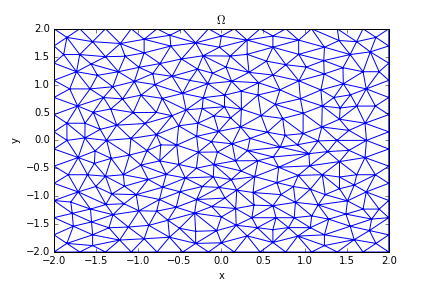
\includegraphics[width=0.5\textwidth]{Figures/tri_mesh.png}
	\end{center}
	\caption{A triangulated mesh $\Omega_h \in [-2,2]^2$, consisting of $546$ elements.}
	\label{fig:tri_mesh}
\end{figure}
To compute the integral of a function $F$ over $\Omega_h$, we simply add the value of the integral at each individual element. That is:
\begin{equation}\label{eqn:gquad_tmesh}
\iint_{\Omega} F(x, y) dxdy \approx \sum_{\kappa=1}^{Nt} A_{\kappa}\sum_{j=1}^{Ng} \rho_{j, \kappa} F(\varphi^{\kappa}_x(\hat x_j,\hat y_j), \varphi^{\kappa}_y(\hat x_j,\hat y_j)).
\end{equation}

\subsubsection{A brief example}
Lets work a brief example about integrals in triangulated meshes. Suppose we have a rectangular region $\Omega \in [-2,2]^2$. A triangulation $\Omega_h$ looks like in Figure \ref{fig:tri_mesh}. We want to compute the integral of $f(x,y) = x^2 + y^2$ over $\Omega$. That is, we want
\begin{equation}
\int_{\Omega} (x^2 + y^2) dxdy = \frac{128}{3}.
\end{equation}
The plot of $f$ on $\Omega_h$ is shown in Figure \ref{fig:f_tri_mesh}.

\begin{figure}[H]
	\begin{center}
		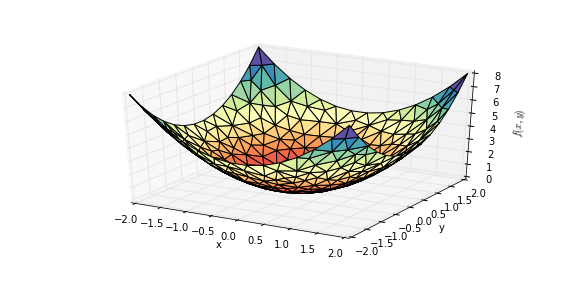
\includegraphics[width=0.6\textwidth]{Figures/f_tri_mesh.png}
	\end{center}
	\caption{Plot of $f(x,y) = x^2 + y^2$ over $\Omega_h$.}
	\label{fig:f_tri_mesh}
\end{figure}

Since $f$ has degree 2, a Gaussian Quadrature with $N_g=2$ should provide an exact integral. A simple for loop which accumulates the value of the integral at each element should provide the correct answer, as shown in Listing \ref{lst:quad_for}. Once the for loops finishes, it returns $42.666666666666679$, which is $\frac{128}{3}$. The complete code can be found in Appendix \ref{app:gauss_quad}.

\begin{listing}[H]
	\centering
	\setminted{fontsize=\small,baselinestretch=1}
\begin{minted}{python}
	
	# Function to integrate over 
	def f(x, y): return x**2 + y**2
	N = 2 # Point rule of the Quadrature
	S = 0
	# Iterate through each element
	for elem in elems:
		# Get vertices of the element
		v1,v2,v3 = mesh_pts[elem]
		# Accumulate the value of the integral for this element.
		S += gaussIntTriangle(f, N, v1 ,v2, v3)
\end{minted}
\caption{python for loop that computes the integral of $f$ over a region consisting of triangular elements. Here we assume that we already have a set of elements and the x,y coordinates of each vertex, given in the mesh points list.}
\label{lst:quad_for}
\end{listing}

\subsection{Nystr\"om Discretization on a Triangulated Mesh}
\label{subsec:tri nystrom discretize}

We start by posing the Wilson-Cowan-Amari Neural Field equation on a two dimensional domain $\Omega \in \mathbb{R}^2$. The equation looks like:
\begin{equation} \label{eqn:2d_tri_nf_gral}
\frac{\partial u(\mathbf{x},t)}{\partial t} = - u(\mathbf{x},t) + \int_{\Omega} W(\mathbf{x},\mathbf{y})f(u(\mathbf{y}, t)) d\mathbf{y}, \hspace{3mm} \mathbf{x} \in \mathbb{R}^2.
\end{equation}
Now $\mathbf{x}$ and $\mathbf{y}$ are vectors with two components, in other words $(\mathbf{x}, \mathbf{y}) \in \mathbb{R}^2$.
The Connectivity Kernel function is defined by:
\begin{equation}\label{eqn:2d_tri_kernel}
W(\mathbf{x},\mathbf{y})  = e^{-b||\mathbf{x}-\mathbf{y}||_2}(b\hspace{1mm} \sin(||\mathbf{x}-\mathbf{y}||_2) + \cos(||\mathbf{x}-\mathbf{y}||_2)),
\end{equation}
and the firing rate function by:
\begin{equation}\label{eqn:2d_tri_frate}
f(u) = \frac{1}{1+e^{-\mu u + \theta}} -\frac{1}{1+e^\theta},
\end{equation}
as usual, $b$ and $\mu$ control the decay of the synaptic kernel and the slope of the sigmoidal firing rate respectively, while $\theta$ is a threshold value. 

Recall that Nystr\"om method was originally introduced to compute approximations based on numerical integration of the integral operator on Fredholm integral equations of the second kind.

Then, following the lines presented in the book by Kendall Atkinson \cite{atkinson1976survey}, we can apply Nystr\"om method to the Neural Field Equation in a similar way as we did for the one dimensional case, but now using the quadrature rule for triangular elements developed in Section \ref{subsec:gquad_t_elems}.

We begin discretizing the domain by covering it with $N_t$ number of triangles $\kappa$, such that $\Omega_h = \bigcup_{i=1}^{N_t} \kappa_{i}$. Recall that the composite integration rule over an element $\kappa$ is given by:
\begin{equation}
\int_{\kappa} F(\mathbf{x}) d\mathbf{x} \approx A_{\kappa} \sum_{j=1}^{Ng} \rho_j F(\varphi(\mathbf{\hat{x}}_j)), \hspace{3mm} \mathbf{x} \in \mathbb{R}^2,
\end{equation} 
as in \ref{eqn:gquad_elem}. 
The quadrature nodes $\{\mathbf{\hat x}_1,...,\mathbf{\hat x}_{N_g}\}$ are contained in a reference triangle $\hat \kappa$, and $\varphi^{\kappa} : \hat{\kappa} \rightarrow \kappa$ is a mapping function that takes any point inside the reference triangle $\hat{\kappa}$ to the triangle $\kappa$, as in equation \ref{eqn:tri_mapping}. 
That is, $\varphi^{\kappa}(\mathbf{\hat{x}}) = \mathbf{v}_1N_1(\mathbf{\hat{x}}) + \mathbf{v}_2N_2(\mathbf{\hat{x}}) + \mathbf{v}_3N_3(\mathbf{\hat{x}})$, where $N_1, N_2, N_3$ are the nodal basis functions defined in \ref{eqn:nodal_basis}, and $\mathbf{v}_i = (x_i, y_i), i=1,2,3$ are the vertices of the triangle $\kappa$. 

For simplicity we define $\varphi^{\kappa}_j=\varphi^{\kappa}(\mathbf{\hat{y}}_j)$. Our domain is now comprised of a set of points, such that: 
\begin{equation}\label{eqn:space_int_ps}
\Omega_h = \{\varphi^{\kappa}_j\}, \hspace{5mm} \kappa = 1,...,N_t; j=1,...,N_g,
\end{equation}
then $\Omega_h \in \mathbb{R}^{N \times 2}$, where $N=N_tN_g$.
Approximating the integral operator in equation \ref{eqn:2d_tri_nf_gral} we get:
\begin{equation}\label{eqn:2d_nf_2}
\frac{\partial u(\mathbf{x},t)}{\partial t} \approx - u(\mathbf{x},t) + \sum_{\kappa=1}^{N_t} A_{\kappa}\sum_{j=1}^{N_g} W(\mathbf{x},\varphi^{\kappa}_j)f(u(\varphi^{\kappa}_j, t)) \rho_j.
\end{equation}
We now let $\mathbf{x}$ run through the grid points to get the fully discretized version of equation \ref{eqn:2d_tri_nf_gral}:
\begin{equation}\label{eqn:2d_nf_3}
\dot{u}(\varphi^{\kappa}_i,t) \approx - u(\varphi^{\kappa}_i,t) + \sum_{\kappa=1}^{N_t} A_{\kappa}\sum_{j=1}^{N_g} W(\varphi^{\kappa}_i,\varphi^{\kappa}_j)f(u(\varphi^{\kappa}_j, t)) \rho_j.
\end{equation}

\subsection{Computational Implementation}
\label{subsec:tri_comp_implem}

The above discretized equation for obtaining solutions of the two-dimensional neural field in a triangulated mesh was implemented using python.

The first step is to build the triangulated mesh $\Omega_h$. For this we used ``MeshPy"\footnote{MeshPy is a package developed by Andreas Kl\"ockner, which offers quality triangular and tetrahedral mesh generation for python. For more information see: https://mathema.tician.de/software/meshpy/} python package.

A triangulated mesh consists of an elemental connectivity array $C_{\kappa}$, and an array of vertices $V_{\kappa}$.

\begin{equation} \renewcommand{\arraystretch}{0.5}
C_{\kappa} = \left[ 
 	\begin{array}{ccc}
	4& 5& 3\\
	5& 7& 8\\
	1& 2& 3\\
	3& 5& 8\\
	7& 1& 8\\
	8& 1& 3\\
	0& 1& 7\\
	7& 5& 6\\
	\end{array} 
\right],
%
\hspace{6mm}
V_{\kappa}=\left[ 
	\begin{array}{cc}
	 2 & 2 \\
	 1 & 2 \\
	0 & 2 \\
	0 & 1 \\
	0 & 0 \\
	1 & 0 \\
	2 & 0 \\
	2 & 1 \\
	1 & 1
	\end{array} ,
\right]
\end{equation}
such that $C_{\kappa}$ are the vertices numbering of each element, and $V_{\kappa}$ are the vertices $(x,y)$ coordinates. See Figure \ref{fig:connectivity}.

\begin{figure}[H]
	\begin{center}
		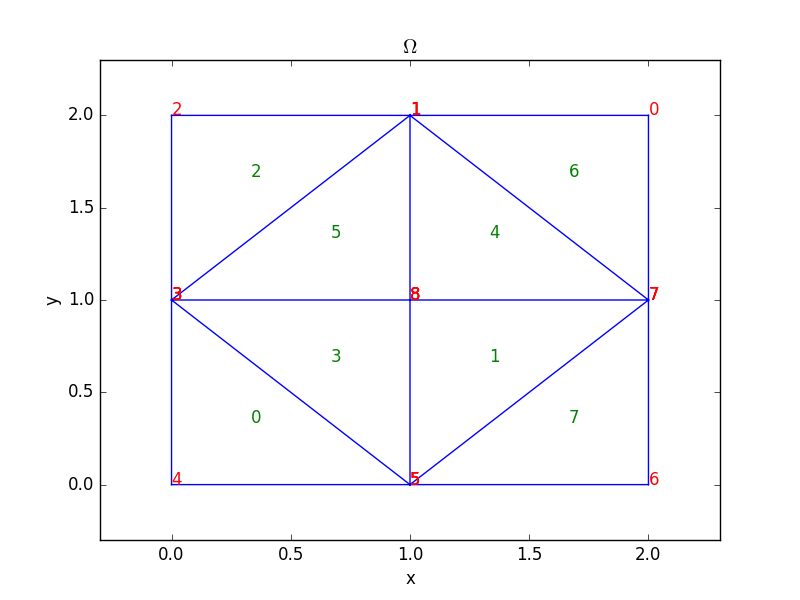
\includegraphics[width=0.5\textwidth]{Figures/Connectivity.png}
	\end{center}
	\caption{A mesh with its connectivity numbering. Green is the number of element, red are the connectivity vertices that correspond to the entry in the vertices array $V_{\kappa}$}
	\label{fig:connectivity}
\end{figure}
For instance, the element at the top of $C_{\kappa}$ consists of the vertices enumerated as $[4,5,3]$, which correspond to the entries $[0,0],[1,0],[0,1]$ in the vertices array $V_{\kappa}$, and are indeed the coordinates of its vertices.

Once we have a triangulated mesh, the next step is to get the Gaussian weights and interior points of a reference triangle and map them inside each element using equation \ref{eqn:tri_mapping}. The Gaussian weights and points are obtained with the function in Appendix \ref{app:gauss_ws_and_ps}. Taking the same example as above, and with a quadrature rule of precision $N=2$ which calls for three interior points, the mesh looks like in Figure \ref{fig:int_points}.
\begin{figure}[H]
	\begin{center}
		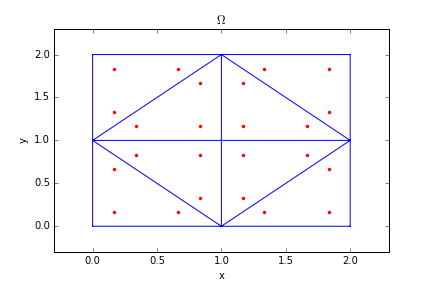
\includegraphics[width=0.5\textwidth]{Figures/interior_points.png}
	\end{center}
	\caption{A mesh with its interior Gauss quadrature nodes for a $2$ precision rule}
	\label{fig:int_points}
\end{figure}
We store each interior point on an array which now corresponds to our new mesh of interior points, such that
\begin{equation}
\Omega_h = \{\varphi^{\kappa}_j\}, \hspace{5mm} \kappa = 1,...,N_t; j=1,...,N_g,
\end{equation}
as in \ref{eqn:space_int_ps}. See the function in Listing \ref{fig:buildMesh_pseudo}

\begin{listing}[H]
	\begin{center}
		\begin{minted}{python}
def buildMesh(conn_mat, vertices, x_hat, y_hat):
	"""
	conn_mat is the Connectivity Array C_{\kappa}
	vertices is the Vertices Array V_{\kappa}
	x_hat, y_hat are the Gauss points inside a 
		reference triangle \hat \kappa
	"""
	for l, elem in enumerate(conn_mat):
		v1,v2,v3 = vertices[elem]
		A[l] = computeArea(v1,v2,v3)
		for j in range(Ng):
			mesh[j] = mapX(v1,v2,v3,x_hat[j],y_hat[j])
		\end{minted}	
	\end{center}
	\caption{Python function for creating the new mesh of interior points.}
	\label{fig:buildMesh_pseudo}
\end{listing}
Now that we have our mesh, we can compute the right-hand side of the discretized equation \ref{lst:computeF_pseudo}. That way we get a time dependant system of ordinary differential equations, and we can study the behaviour of neurons by evolving the equation forward in time using a fourth-order Runge-Kutta (RK4) scheme. In this work we use the Runge-Kutta4 algorithm provided by \texttt{scipy.integrate.ode} package. For information about RK4 algorithm see \cite{heath2002scientific} section 9.6.2.

In search of efficiency, we explored two different approaches for computing the right-hand side of equation \ref{eqn:2d_nf_3}.

A first approach was by means of for loops, iterating through each point in the mesh to make one evaluation of the right-hand side. See the function in Listing \ref{lst:computeF_pseudo}.

\begin{listing}[H]
		\begin{minted}{python}
def computeF(u, mesh, As, w, f, rho):
	"""
	One evaluation of the right hand side.
	Receives:
		u -> cuerrent state vector to evaluate at
		mesh -> mesh of interior points
		As -> Vector of Areas of each element
		w -> Synaptic connectivity function
		f -> firing rate function
		rho -> Weights for the Gauss Quadrature rule
	"""
	N = xs.shape[0] # Length of the mesh
	Nt = len(A) # Number of elements
	Ng = len(rho) # Number of Gauss Points
	F = np.zeros(n)
	
	for i in range(N):
		S = 0.0
		for l in range(Nt):
			sigma = 0
			for j in range(Ng):
				k = l*nG + j
				sigma += w(xs[i]-xs[k])*f(u[k])*rho[j]
			S += sigma*A[l]
		F[i] = - u[i] + S
	return F
		\end{minted}	
	\caption{Python function for evaluating the right hand side of the discretized Neural Field Equation using for loops.}
	\label{lst:computeF_pseudo}
\end{listing}
This approach is a direct implementation of eq. \ref{eqn:2d_nf_3}. Each evaluation of the right-hand side takes $O(N^2)$ operations, where $N=NtNg$, with $Nt$ being the number of elements in the mesh, and $Ng$ the number of Gauss interior points.

With this approach we found that, for more refined meshes ($Nt \rightarrow \infty$), the algorithm becomes extremely slow. That is due to the number of right-hand side operations being performed, and the complexity of each evaluation. Each time step of the RK4 algorithm needs 4 evaluations of the right-hand side, each costing $O(N^2)$ operations.

The second approach we took was by pre-building a ``Synaptic Matrix" $\mathbf{W}$, and computing the right-hand side by matrix-vector multiplication. To visualize this approach we transform eq.\ref{eqn:2d_nf_3} to a matrix-vector equation using the synaptic matrix $\mathbf{W}$ as
\begin{equation}\label{eqn:2d_tri_mat-vec}
\dot{\textbf{u}}(t) = - \textbf{u}(t) + \textbf{W} \hspace{1mm} \textbf{f}(\textbf{u}(t)), \hspace{3mm} \textbf{W} \in \mathbb{R}^{N \times N}, \textbf{u} \in \mathbb{R}^{N},
\end{equation}
with $N=N_tN_g$, where
\begin{subequations}\label{eqn:2d_tri_w&f}
	\begin{align}
		\mathbf{W}_{i,j} &= W(\varphi^{\kappa}_i, \varphi^{\kappa}_j) A_{\kappa} \rho_j , 
		\hspace{3mm} \textnormal{and}\\
		\textbf{f}(\mathbf{u}_i(t)) &= f(u(\varphi^{\kappa}_i,t))
		\hspace{3mm} \forall \hspace{1mm} i,j = 0,...,N,
	\end{align}
\end{subequations}
This way we can build $\mathbf{W}$ just once, and then test the model changing parameters and initial conditions using the same matrix $\mathbf{W}$ every time.

As in the 2D case, we can halve the time it takes to assemble $\mathbf{W}$ by using the symmetry of the synaptic connectivity kernel ($W(\textbf{x}, \textbf{y}) = W(\textbf{y},\textbf{x})$) and by exploiting the efficiency of python's \texttt{numpy} package. That is, we can compute the values of $\mathbf{W}$ just for the upper triangular part, and then device a strategy to efficiently copy the upper triangular values to the lower triangular part of $\mathbf{W}$. After that we multiply times a vector that contains the values of the Areas and quadrature weights $A_{\kappa}\rho_j, \hspace{3mm} \kappa=1,...,N_t, j=1,...,N_g$. A function that builds the synaptic matrix $\mathbf{W}$ is included in Listing \ref{lst:buildW} below.

\begin{listing}[H]
		\begin{minted}{python}
def buildW(mesh, Areas, weights, kernel):
	"""
	Assemble the Synaptic Matrix W.
	Receives:
		mesh -> mesh of interior points
		Areas -> Vector of Areas of each element (numpy array)
		weights -> Weights for the Gauss Quadrature rule (numpy array)
		kernel -> Synaptic connectivity kernel function (callable function)
	"""
	# Vector of areas and weights
	rhos = numpy.outer(Areas.T, weights)
	rhos = rhos.flatten()
	N = len(mesh); W = np.zeros( (N,N) )
	# Compute only the upper triangular part
	for i in range(0, N):
		x_pt = xs[i]
		for j in range(i, N):
			y_pt = xs[j]
			x, y = x_pt-y_pt
			W[i,j] = kernel(x, y) 
	
	# Copy upper triangular part to lower triangular part
	i_lower = numpy.tril_indices(N, -1)
	W[i_lower] = W.T[i_lower]
	
	W *= rhos # Multiply times the weights
	return W
		\end{minted}	
	\caption{Pseudo Code for building the Synaptic Matrix $\mathbf{W}$.}
	\label{lst:buildW}
\end{listing}

Once assembled the Synaptic Matrix $\mathbf{W}$, a right-hand side evaluation of the discretized equation, as usual, consists of a matrix-vector multiplication as in Listing \ref{lst:computeF_synMat}.

\begin{listing}[H]
		\begin{minted}{python}
def computeF(u, f_rate, W):
	"""
	One evaluation of the right hand side.
	Receives:
		u -> cuerrent state vector to evaluate at
		W -> pre computed Synaptic Matrix
		f_rate -> callable firing rate function
	"""
	f_u = f_rate(u) # Evaluate firing rate at u
	return -u + (W).dot(f_u)

		\end{minted}	
	\caption{Python function for evaluating the right hand side of the discretized Neural Field Equation using a pre built Synaptic Matrix $\mathbf{W}$.}
	\label{lst:computeF_synMat}
\end{listing}

With the function to compute the right hand side of eq.\ref{eqn:2d_tri_mat-vec} we can proceed with the time stepping using RK4 algorithm to find localised bump solutions. In this work we use the Runge-Kutta4 algorithm provided by \texttt{scipy.integrate.ode} package. For information about RK4 algorithm see \cite{heath2002scientific} section 9.6.2.

\subsection{Numerical Experiments} \label{subsec:tri_num_experiments}
In this section we test the developed algorithm by running some numerical experiments with the objective of measuring the error as the mesh is refined, that is, as we include more triangular elements in the mesh. 

Before proceeding we must define how the spacing between nodes $h$ is defined for this instance of the problem. Recall that the discretized $\Omega$ is comprised of elements having interior Gauss points, such that $\Omega_h=\{\varphi_j^{\kappa}\}$ for $\kappa = 1,...,N_t$ and $j = 1,...,N_g$, with $N_t$ being the total number of elements , and $N_g$ the effective number of Gauss interior points used to discretize the mesh; as in eqn. \ref{eqn:space_int_ps}. A picture of the actual triangulated mesh with interior Gauss points used for this numerical experiments is shown in fig. \ref{fig:tri_mesh_3Gpoints}

\begin{figure}[H]
	\begin{center}
	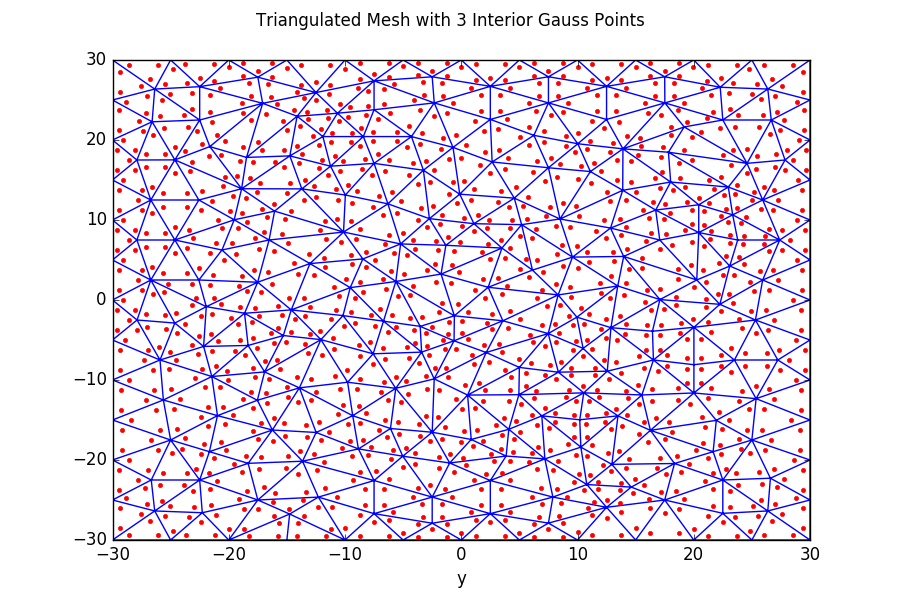
\includegraphics[width=0.8\textwidth]{Figures/Mesh_With_3_Interior_Points.png}
	\end{center}
	\caption{Discretized mesh $\Omega_h$ comprised of $N_t=546$ triangular elements and $N_g=3$ interior Gauss points.}
	\label{fig:tri_mesh_3Gpoints}
\end{figure}
The spacing between nodes in a triangulated mesh is defined as
\begin{equation} \label{eqn:tri_h_kappa}
h_{\kappa} = \max_{\kappa \in \Omega_h} D_{\kappa},
\end{equation}
where $D_{\kappa}$ is the diameter of the $\kappa$-th element. The diameter of a triangle is the length of its longest edge (blue lines). If we now introduce interior Gauss points (red dots), then we must create a new triangulation using the Gauss points (red) as vertices for new triangles, therefore having new edges. Then the spacing between points is defined as 
\begin{equation}
\tilde{h}_{\kappa} = \max_{\kappa \in \Omega_h} \tilde{D}_{\kappa},
\end{equation}
where $\tilde{D}_{\kappa}$ is the diameter of the new $\kappa$-th element formed by triangulating the interior Gauss points. However, note that $h_{\kappa}$ and $\tilde{h}_{\kappa}$ scale asymptotically in the same way as the mesh is refined. So, for means of studying the convergence of the errors for more refined meshes we can make use of $h_{\kappa}$ as defined in eqn. \ref{eqn:tri_h_kappa}.

Now we proceed with the numerical experiments. We use the same examples as for the 2D model in section \ref{subsec:2d_tests}, which were drawn from Lima and Buckwar paper \cite{lima2015numerical} section 3.

\textit{Example 1.} Recall that for this example, the connectivity kernel is given by
\begin{equation}\label{eqn:tri_test1_W}
W(\textbf{r},\textbf{r'}) = W(x_1,y_1,x_2,y_2) = \exp\left(-\lambda (x_1- y_1)^2 - \lambda (x_2-y_2)^2\right), \hspace{3mm} \lambda \in \mathbb{R}^+.
\end{equation}
The firing rate function by
\begin{equation}\label{eqn:tri_test1_frate}
f(\mathbf{u}) = \tanh(\sigma \mathbf{u}), \hspace{3mm} \sigma \in \mathbb{R}^+,
\end{equation}
and we incorporate en external input $I_{ext}$ given by
\begin{equation}\label{eqn:tri_test1_Iext}
I_{ext}(x,y,t) = -\tanh\left( \sigma \exp \left( -\frac{t}{c}\right)\right) b(x_1,y_1;\lambda),
\end{equation}
where
\begin{equation}\label{eqn:tri_test1_b}
\begin{split}
b(x_1,y_1;\lambda) &= \int_{-1}^{1} \int_{-1}^{1} W(x_1,y_1,x_2,y_2)dy_1dy_2\\
&=\frac{\pi}{4\lambda}\left( \textnormal{Erf}(\sqrt{\lambda}(1-x_1)) + \textnormal{Erf}(\sqrt{\lambda}(1+x_1))\right) \left( \textnormal{Erf}(\sqrt{\lambda}(1-x_2)) + \textnormal{Erf}(\sqrt{\lambda}(1+x_2))\right),
\end{split}
\end{equation}
with Erf being the Gaussian error function.
For this case, the exact solution is
\begin{equation}\label{eqn:tri_test1_exactsol}
u(\textbf{r}, t) = \exp \left( - \frac{t}{c}\right).
\end{equation}

The objective is to measure the error for a more refined triangulated mesh $\Omega_h$. The error is defined as the difference between the true solution $u(\mathbf{x}, t)$ and the computed solution $u_h(\mathbf{x}, t)$ using a mesh refinement of $h$ as defined in eqn.\ref{eqn:tri_h_kappa}. That means
\begin{equation}\label{eqn:tri_numexp_errormeasure}
	e_T(h) = \| u(\mathbf{x}, T) -  u_h(\mathbf{x}, T)\|_{\infty}, \hspace{3mm} \mathbf{x}\in\mathbb{R}^2
\end{equation}
is the error measured at the final time $T$ that depends on the mesh refinement $h$. We start the time stepping with an initial condition given by
\begin{equation}
	u(\mathbf{x}, 0) \equiv 1,
\end{equation}
from the initial time $t=0$ to the final time $T=1$ with a time step size of $h_t = 0.1$.

A Gaussian quadrature with precision rule $q$ has an integration error of order $h^{2q}$. Therefore, using a precision rule of order $q=2$ we expect a behaviour of the type
\begin{equation}\label{eqn:tri_numexp_errormeasure2}
e_T(h) = \| u(\mathbf{x}, T) -  u_h(\mathbf{x}, T)\|_{\infty} = O(h^4) \hspace{3mm}
\textnormal{as} \hspace{3mm} h \rightarrow \infty,
\end{equation}
where $h$ is the spacing between nodes as defined in \ref{eqn:tri_h_kappa}. For a proof of this sentence see \cite{lima2015numerical} section 2.1.2, theorem 2.4.

Table \ref{table:2dTri_Errors_test1_q2} contains the measure of the errors $e_T(h)$ for more refined triangular meshes. First column $N_t$ are the number of triangles, second column $N$ are the total number of points in the mesh ($N = N_tN_g$) where $N_g$ are the number of Gauss interior points, third column $h$ contains the spacing between vertices of triangles as defined in eqn. \ref{eqn:tri_h_kappa}, and fourth column $e_T(h)$ is the error measure as in eqn. \ref{eqn:tri_numexp_errormeasure}. While figure \ref{fig:2dTri_Errors_test1_q2} displays the error measures $e_T(h)$ (blue dots) against an actual $h^4$ curve (red line), providing numerical evidence on an $O(h^4)$ behaviour.
\begin{table}[H]
	\centering
	\begin{tabular}{|c|c|c|c|}
		\hline
		$N_t$&$N$&$h$&$e_T(h)$\\
		\hline
		50&150&0.5&2.89e-05\\
		74&222&0.4&2.12e-05\\
		114&342&0.333&1.10e-05\\
		152&456&0.286&5.05e-06\\
		192&576&0.25&2.25e-06\\
		252&756&0.222&2.22e-06\\
		308&924&0.2&1.31e-06\\
		382&1146&0.182&9.41e-07\\
		450&1350&0.167&6.05e-07\\
		516&1548&0.154&5.41e-07\\
		\hline
	\end{tabular}
	\caption{Table containing the errors of \textit{example 1} for a more refined mesh grid using a two precision rule $q=2$, which calls for three Gauss interior points $N_g=3$. Parameters were set as $\lambda=1$, $\sigma=1$, $c=1$.}
	\label{table:2dTri_Errors_test1_q2}
\end{table}

\begin{figure}[H]
	\begin{center}
		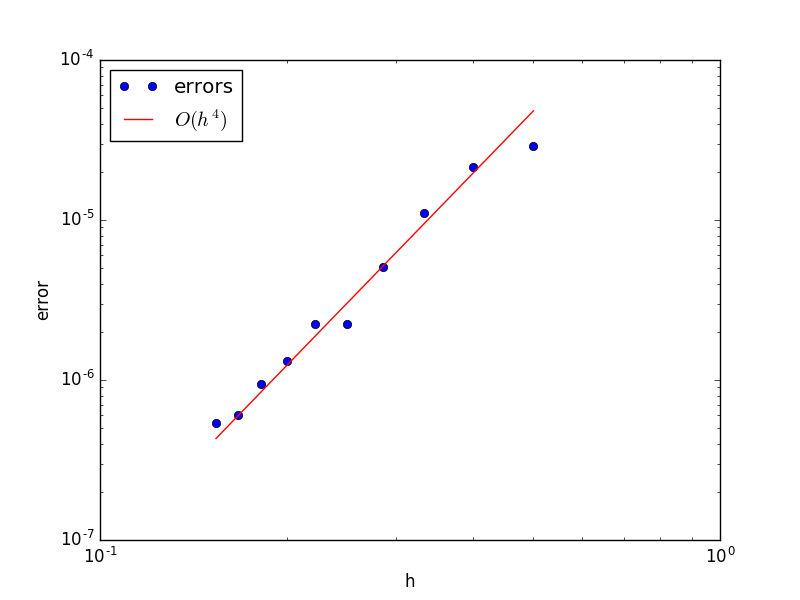
\includegraphics[width=0.7\textwidth]{Figures/2dTriTest1_q=2,Ng=3.png}
	\end{center}
	\caption{Plot of errors v.s. an actual $h^4$ curve for \textit{example 1} using a two precision rule $q=2$, which calls for three Gauss interior points $N_g=3$, on a log-log scale. Mesh refinement $h$ on the $x$-axis, error measures on the $y$-axis. Parameters were set as $\lambda=1$, $\sigma=1$, $c=1$.}
	\label{fig:2dTri_Errors_test1_q2}
\end{figure}

Taking the same \textit{example 1} but now with a four precision rule $q=4$, then we expect an $O(h^8)$ behaviour, meaning that
\begin{equation}
e_T(h) = \| u(\mathbf{x}, T) -  u_h(\mathbf{x}, T)\|_{\infty} = O(h^8) \hspace{3mm}
\textnormal{as} \hspace{3mm} h \rightarrow \infty,
\end{equation}
where $h$ is the spacing between nodes as defined in \ref{eqn:tri_h_kappa}. For a proof of this sentence see \cite{lima2015numerical} section 2.1.2, theorem 2.4. Table \ref{table:2dTri_Errors_test1_q4} contains the error measures $e_T(h)$ for more refined mesh grids. Figure \ref{} shows the error measures $e_T(h)$ (blue dots) against an actual $h^8$ curve (red line), providing numerical evidence on an $O(h^8)$ behaviour.

\begin{table}[H]
	\centering
	\begin{tabular}{|c|c|c|c|}
		\hline
		$N_t$&$N$&$h$&$e_T(h)$\\
		\hline
		50&350&0.5&8.49e-08\\
		74&518&0.4&6.85e-08\\
		114&798&0.333&1.33e-08\\
		152&1064&0.286&6.37e-09\\
		192&1344&0.25&2.09e-09\\
		252&1764&0.222&9.92e-10\\
		\hline
	\end{tabular}
	\caption{Table containing the errors of \textit{example 1} for a more refined mesh grid using a four precision rule $q=4$, which calls for five Gauss interior points $N_g=5$. Parameters were set as $\lambda=1$, $\sigma=1$, $c=1$.}
	\label{table:2dTri_Errors_test1_q4}
\end{table}

\begin{figure}[H]
	\begin{center}
		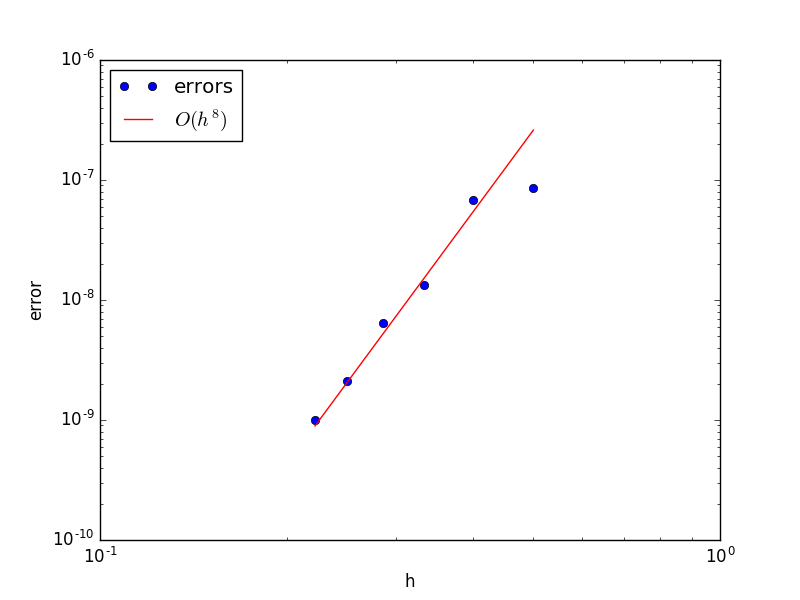
\includegraphics[width=0.7\textwidth]{Figures/2dTriTest1_q=4,Ng=5.png}
	\end{center}
	\caption{Plot of errors v.s. an actual $h^8$ curve for \textit{example 1} using a four precision rule $q=4$, which calls for five Gauss interior points $N_g=5$, on a log-log scale. Mesh refinement $h$ on the $x$-axis, error measures on the $y$-axis. Parameters were set as $\lambda=1$, $\sigma=1$, $c=1$.}
	\label{fig:2dTri_Errors_test1_q4}
\end{figure}

\textit{Example 2.} For this second example we take the same equation \ref{eqn:tri_test1_W} for $W$, and \ref{eqn:tri_test1_frate} for the firing rate $f$. We change the external input to be
\begin{equation}
	I_{ext} = c + t - \tanh(\sigma t)b(x,y;\lambda),
\end{equation}
with $b$ as in eqn. \ref{eqn:tri_test1_b}. We will carry the same analysis as in \textit{example 1} except that we are now going to vary the parameters $\lambda$, $\sigma$, $c$. We will stick with a two precision rule $q = 2$, which calls for $N_g = 3$ interior points, therefore we expect an $O(h^4)$ behaviour on the errors, as in eqn. \ref{eqn:tri_numexp_errormeasure2}.

Table \ref{table:2dTri_Errors_test2_q2} contains measures of the errors $e_T(h)$ as defined in \ref{eqn:tri_numexp_errormeasure}, for more refined triangulated meshes and for three different cases. In case1: $\lambda=1$, $\sigma=1$, $c=1$, case2 is when $\lambda=1$, $\sigma=5$, $c=1$, and case 3 is with a $\lambda=5$, $\sigma=5$, $c=1$. Figures \ref{fig:2dTri_Errors_test2_case1}-\ref{fig:2dTri_Errors_test2_case2}-\ref{fig:2dTri_Errors_test2_case3} show the error measures $e_T(h)$ (blue dots) on top of an actual $h^4$ curve (red line) for the three different cases. Notice how the three cases display an $O(h^4)$ behaviour, providing evidence that the algorithm is correct.


\begin{table}[H]
	\centering
	\begin{tabular}{|c|c|c|c||c|c|c|c||c|c|c|c||}
		\hline
		\multicolumn{4}{|c||}{Case 1}&
		\multicolumn{4}{|c||}{Case 2}&
		\multicolumn{4}{|c||}{Case 3}\\
		\multicolumn{4}{|c||}{$\lambda=1$, $\sigma=1$, $c=1$}&
		\multicolumn{4}{|c||}{$\lambda=1$, $\sigma=5$, $c=1$}&
		\multicolumn{4}{|c||}{$\lambda=5$, $\sigma=5$, $c=1$}\\
		%\hline
		$N_t$&$N$&$h$&$e_T(h)$&
		$N_t$&$N$&$h$&$e_T(h)$&
		$N_t$&$N$&$h$&$e_T(h)$\\
		\hline \hline
		50&150&0.5&2.51e-05&
		50&150&0.5&3.86e-05&
		50&150&0.5&0.0005\\
		74&222&0.4&1.84e-05&
		74&222&0.4&2.82e-05&
		74&222&0.4&0.0003\\
		114&342&0.333&9.23e-06&
		114&342&0.333&1.38e-05&
		114&342&0.333&8.07e-05\\
		152&456&0.286&4.18e-06&
		152&456&0.286&6.32e-06&
		152&456&0.286&5.89e-05\\
		192&576&0.25&1.80e-06&
		192&576&0.25&2.66e-06&
		192&576&0.25&2.15e-05\\
		252&756&0.222&1.76e-06&
		252&756&0.222&2.57e-06&
		252&756&0.222&1.31e-05\\
		308&924&0.2&1.05e-06&
		308&924&0.2&1.54e-06&
		308&924&0.2&8.38e-06\\
		382&1146&0.182&7.55e-07&
		382&1146&0.182&1.11e-06&
		382&1146&0.182&7.45e-06\\
		\hline
	\end{tabular}
	\caption{Table containing the errors of \textit{example 2} for a more refined mesh grid using a four point $q=4$ precision rule, for three different cases of parameter values. Case1: $\lambda=1$, $\sigma=1$, $c=1$, Case2: $\lambda=1$, $\sigma=5$, $c=1$, Case3: $\lambda=5$, $\sigma=5$, $c=1$.}
	\label{table:2dTri_Errors_test2_q2}
\end{table}

\begin{figure}[H]
	\begin{center}
		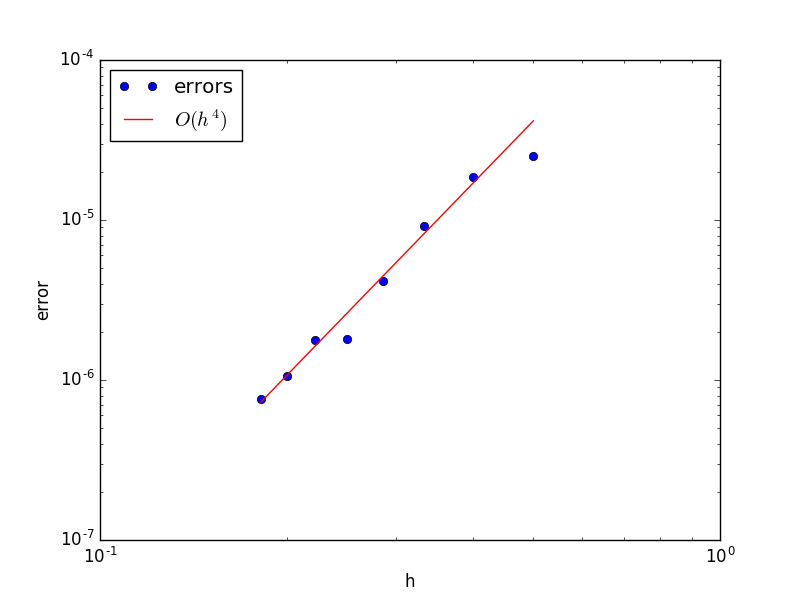
\includegraphics[width=0.7\textwidth]{Figures/2dTriTest2_case1.png}
	\end{center}
	\caption{Plot of errors v.s. an actual $h^4$ curve for \textit{example 2} using a two precision rule $q=2$, which calls for three Gauss interior points $N_g=3$, on a log-log scale. Mesh refinement $h$ on the $x$-axis, error measures on the $y$-axis. Parameters were set as $\lambda=1$, $\sigma=1$, $c=1$.}
	\label{fig:2dTri_Errors_test2_case1}
\end{figure}

\begin{figure}[H]
	\begin{center}
		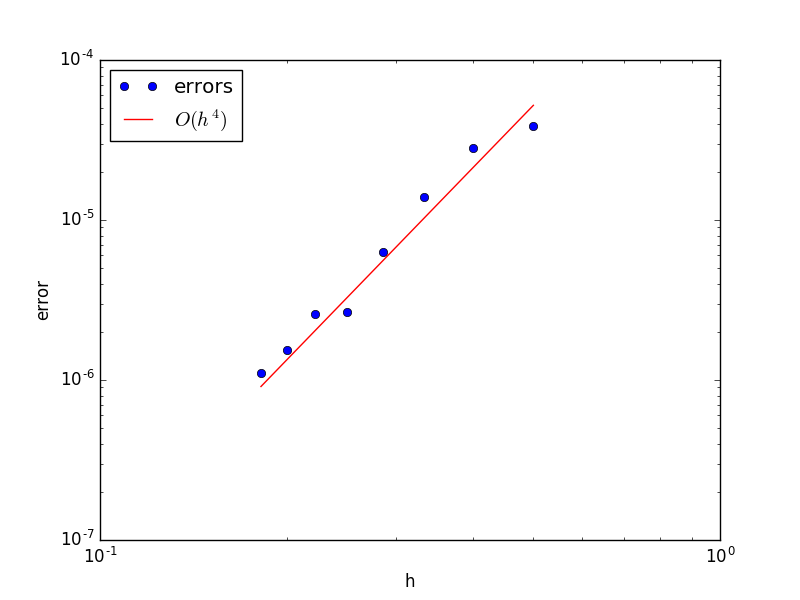
\includegraphics[width=0.7\textwidth]{Figures/2dTriTest2_case2.png}
	\end{center}
	\caption{Plot of errors v.s. an actual $h^4$ curve for \textit{example 2} using a two precision rule $q=2$, which calls for three Gauss interior points $N_g=3$, on a log-log scale. Mesh refinement $h$ on the $x$-axis, error measures on the $y$-axis. Parameters were set as $\lambda=1$, $\sigma=5$, $c=1$.}
	\label{fig:2dTri_Errors_test2_case2}
\end{figure}

\begin{figure}[H]
	\begin{center}
		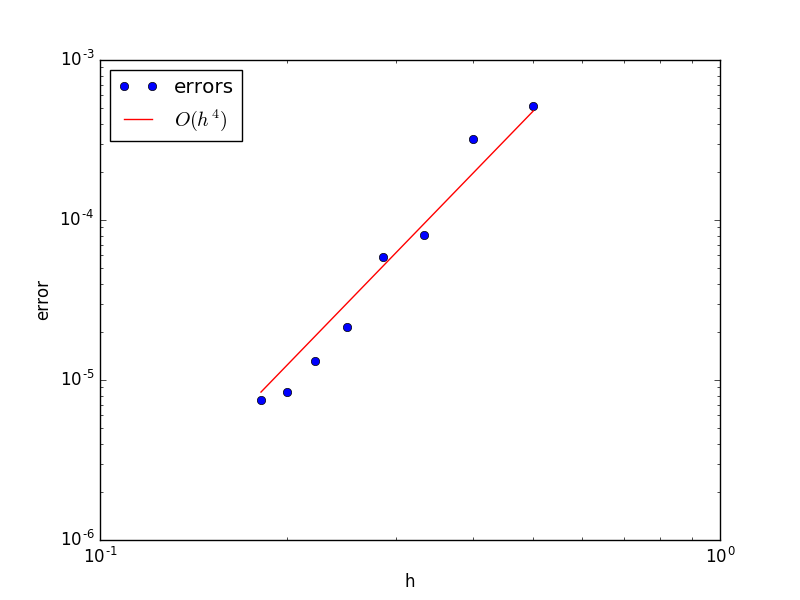
\includegraphics[width=0.7\textwidth]{Figures/2dTriTest2_case3.png}
	\end{center}
	\caption{Plot of errors v.s. an actual $h^4$ curve for \textit{example 2} using a two precision rule $q=2$, which calls for three Gauss interior points $N_g=3$, on a log-log scale. Mesh refinement $h$ on the $x$-axis, error measures on the $y$-axis. Parameters were set as $\lambda=5$, $\sigma=5$, $c=1$.}
	\label{fig:2dTri_Errors_test2_case3}
\end{figure}


\subsection{Results} \label{subsec:tri_results}
In this part we use the algorithm developed throughout this section to find patterns of activity in the form of hexagonal patches and radially-symmetric spots, in the same way as we did in the 2D model \ref{subsec:2d_results}.

In section \ref{subsec:2d_results} we saw how different combinations of initial conditions and control parameters lead to different patterns of activity. In particular we reproduced the result presented in \cite{rankin2014continuation} page 4. Now we use the same conditions and parameters to test this model and draw some conclusions. Namely, we fix $b=0.4$, $\theta=5.6$, and let $\mu$ vary in equations \ref{eqn:2d_tri_kernel}-\ref{eqn:2d_tri_frate}. Time simulations were carried out for $t \in [0,15]$ with a step size of $h_t=0.1$.

Recall that the initial conditions are given by
\begin{subequations}
	\begin{align}
		u(\mathbf{r},0) = u(x,y) &= A \exp \left(-\frac{x^2+y^2}{L}\right), \hspace{3mm} \textnormal{and} \label{eqn:2d_tri_initcond1}\\
		u(\mathbf{r},0) = u(x,y) &= A \exp \left(-\frac{x^2+y^2}{L}\right) \left[ \cos(x) + \cos\left( \frac{1}{2}x + \frac{\sqrt{3}}{2}y\right) + \cos\left( -\frac{1}{2}x + \frac{\sqrt{3}}{2}y\right)\right].\label{eqn:2d_tri_initcond2}
	\end{align}
\end{subequations}
An important finding of this section is that, when using a triangulated mesh, the number of elements used for the discretization heavily impacts the stability properties of the solutions. Rankin and Avitabile, on their paper \cite{rankin2014continuation} show that the choice of the connectivity kernel function $W$ has a considerable impact on the stability properties and on the evolution of the localised states. A change in the discretized connectivity matrix $\mathbf{W}$ is equivalent to changing the connectivity kernel function $W$. In particular, a less refined mesh amounts to having a more sparse connectivity structure, meaning that groups of neurons are less connected between them, and this is equivalent to changing the function $W$. Therefore, using a less refined mesh affects the stability properties and the evolution of the localised states. 
 
We tested the algorithm with two different mesh refinements. For the first refinement we used $N_t=440$ elements and $N_g=3$ interior Gauss points, meaning that the mesh was comprised of $N=1,320$ points. On the second refinement we used $N_t=1,234$ elements and $N_g=3$ interior Gauss points, so that the mesh contained $N=3,702$ points. 
 
We start by analysing the initial bump of activity given by \ref{eqn:2d_tri_initcond1}. Recall how on the 2D model we found that when $\mu \in [4,5]$ the initial bump of activity converges towards a radially-symmetric spot solution, and for $\mu > 5$ the initial bump diverges towards bump solutions that invade the entire domain, as in figure \ref{fig:2dRect_IC1}. 

Now, using the first refinement ($N_t=440$) we found a totally different stationary structure than the one found in the 2D model. In particular, we found that the range of $\mu$ where the initial bump converges to a spatially-localised spot is given when $\mu \in [2,3]$, and for $\mu > 3$ we found the divergence to localised bump solutions that invade the domain, with the speed of divergence growing as $\mu \rightarrow \infty$ (Heaviside case of firing rate). This result is displayed in fig. \ref{fig:2dTri_ic1_440}.

Figure \ref{fig:2dTri_ic1_1234} shows the results with this same initial condition \ref{eqn:2d_tri_initcond1}, but now using the second mesh refinement of $N_t=1,234$ elements. In this case we were able to reproduce the solutions of the 2D model fig. \ref{fig:2dRect_IC1}. Namely, the convergence of a small bump of activity to a localised spot solution when $\mu \in [4,5]$, and a divergence to bump solutions that invade the domain when $\mu > 5$.

\begin{figure}[H]
	\begin{center}
		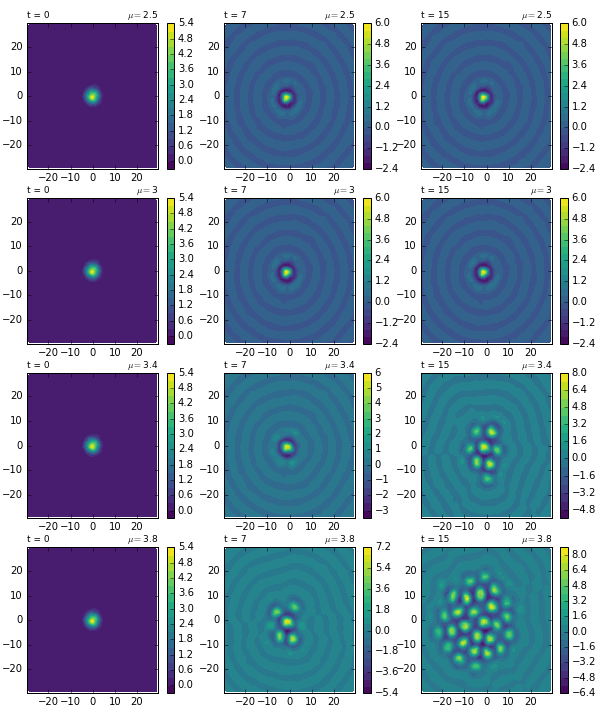
\includegraphics[width=0.8\textwidth]{Figures/2dTri_IC1_440elems.png}
	\end{center}
	\caption{Time simulation of the model \ref{eqn:2d_nf_3} using \ref{eqn:2d_tri_initcond1} as initial condition with $A=6$ and $L=5.77$, with a space discretization of $Nt=440$ elements and $N_g=3$ interior Gauss points. First row displays a convergence towards a radially-symmetric spot with $\mu=2.5$, second row shows the same convergence with $\mu=3.0$, third row displays a divergence towards localised bump solutions with $\mu=3.4$ and the fourth row shows a much faster divergence using $\mu = 3.8$.}
	\label{fig:2dTri_ic1_440}
\end{figure}

\begin{figure}[H]
	\begin{center}
		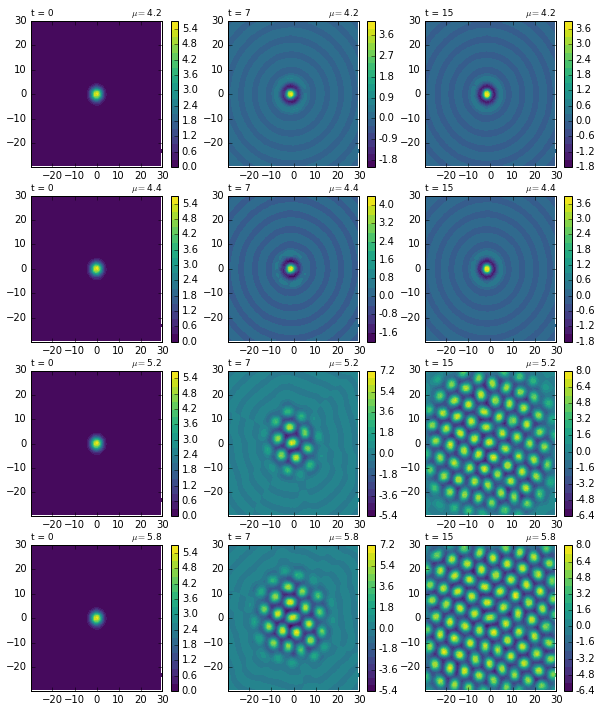
\includegraphics[width=0.8\textwidth]{Figures/2dTri_IC1_1234elems.png}
	\end{center}
	\caption{Time simulation of the model \ref{eqn:2d_nf_3} using \ref{eqn:2d_tri_initcond1} as initial condition with $A=6$ and $L=5.77$, with a space discretization of $Nt=1234$ elements and $N_g=3$ interior Gauss points. All rows display a convergence towards a radially-symmetric spot, first row uses $\mu=3.0$, for the second row $\mu=3.4$, and the third row uses $\mu=3.8$.}
	\label{fig:2dTri_ic1_1234}
\end{figure}

Moving to the second initial condition given by \ref{eqn:2d_tri_initcond2}. In the 2D model, we saw how a hexagonal pattern converges towards a stable localised state when $\mu \in [2.5, 3]$, and that the hexagonal pattern diverges towards localised bump solutions that invade the domain when $\mu > 3$, with the speed of divergence growing as $\mu \rightarrow \infty$ (Heaviside case of firing rate). This results are shown in figure \ref{fig:2dRect_IC2}.

Using a mesh refinement of $N_t = 440$ elements we found that the convergence of this hexagonal pattern to a stable localised state is given when $\mu \in [2, 2.5]$, and the pattern diverges towards invasive spot solutions when $\mu > 2.5$. This results are displayed in figure \ref{fig:2dTri_ic2_440}. 

In figure \ref{fig:2dTri_ic2_1234} we now see how using a mesh refinement of $N_t = 1,234$ elements we are able to reproduce the results of the 2D case. Namely, a convergence of the hexagonal pattern when $\mu \in [2.5, 3]$ and a faster divergence towards invasive spots as $\mu \rightarrow \infty$ (Heaviside case of firing rate).

\begin{figure}[H]
	\begin{center}
		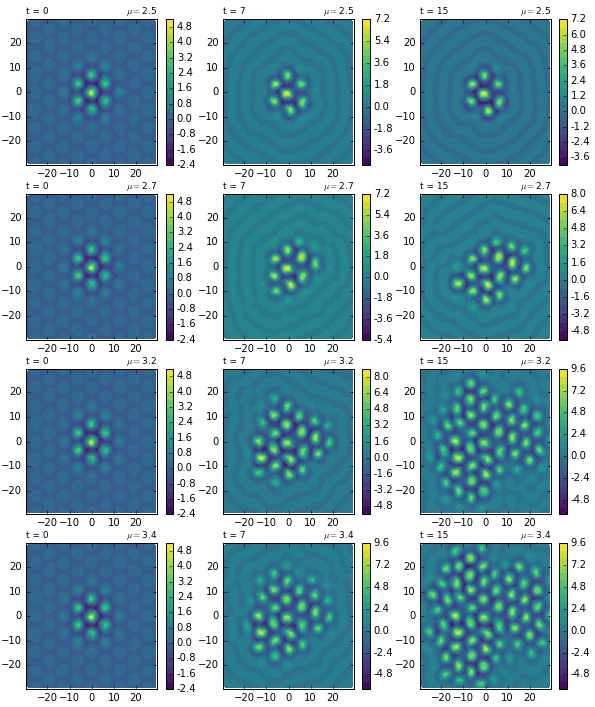
\includegraphics[width=0.8\textwidth]{Figures/2dTri_IC2_440elems.png}
	\end{center}
	\caption{Time simulation of the model \ref{eqn:2d_nf_3} using \ref{eqn:2d_tri_initcond1} as initial condition with $A=6$ and $L=5.77$, with a space discretization of $Nt=440$ elements and $N_g=3$ interior Gauss points. First row displays a stationary hexagonal pattern with $\mu=2.5$, second row shows a divergence towards bump solutions that invade the domain with $\mu=2.7$, third row displays a faster divergence towards invading bump solutions with $\mu=3.2$ and the fourth row shows an even faster divergence using $\mu = 3.4$.}
	\label{fig:2dTri_ic2_440}
\end{figure}


\begin{figure}[H]
	\begin{center}
		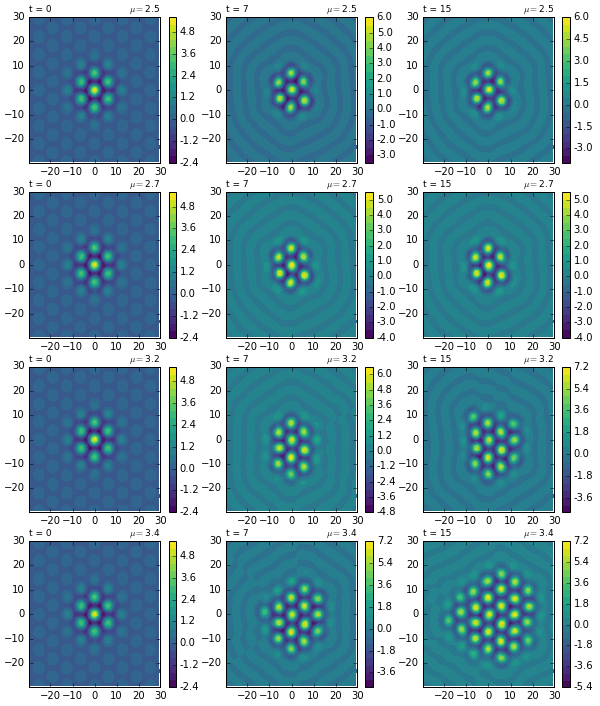
\includegraphics[width=0.8\textwidth]{Figures/2dTri_IC2_1234elems.png}
	\end{center}
	\caption{Time simulation of the model \ref{eqn:2d_nf_3} using \ref{eqn:2d_tri_initcond1} as initial condition with $A=6$ and $L=5.77$, with a space discretization of $Nt=1234$ elements and $N_g=3$ interior Gauss points. First row displays a stationary hexagonal pattern with $\mu=2.5$, second row shows the same stationary pattern using $\mu=2.7$, third row displays a divergence towards bump solutions that invade the domain with $\mu=3.2$ and the fourth row a faster divergence towards invading bump solutions using $\mu = 3.4$.}
	\label{fig:2dTri_ic2_1234}
\end{figure}
%---------------------------------------
\section{The 2D Model with Adaptation} \label{sec:2d_adaptation}
In this section we test the algorithm for triangulated meshes developed in section \ref{sec:nf_t_domain} by solving a Neural Field model that incorporates a spike frequency adaptation current. To compare results we first solve the model on a tensor product mesh using Fast Fourier Transforms and then solve it on a triangulated mesh using Nystr\"om method as developed in section \ref{sec:nf_t_domain}.

We have already seen how two dimensional neural field models can exhibit localised solutions in the form of spots. When a spike frequency adaptation current is added, these models can also support what is called breathers and travelling spot solutions. Some studies that show solutions of this type include \cite{ermentrout2014spatiotemporal,coombes2003waves,coombes2014spots,laingatwo}.

As in \cite{coombes2014spots} we focus on a planar single population model that is written in the form
\begin{subequations}\label{eqn:2d_2component_gral}
	\begin{align}
		\frac{1}{\alpha} \frac{\partial u(\textbf{r},t)}{\partial t} &= -u(\textbf{r},t) + \int_{\mathbb{R}^2} W(\textbf{r},\textbf{r'})f(u(\textbf{r'},t)) d\textbf{r'} - g a(\textbf{r},t)\\
		\frac{\partial a(\textbf{r},t)}{\partial t} &= -a(\textbf{r},t) + u(\textbf{r},t),
	\end{align}
\end{subequations}
with $\textbf{r} \in \mathbb{R}^2$, and $t \in \mathbb{R}^+$. Where, as usual, $u$ represents synaptic activity, $W$ is the synaptic connectivity function, $f$ is the sigmoidal firing rate function, and $a$ is the adaptation function that incorporates a negative local feedback with $g \in \mathbb{R}$ being the strength of the negative feedback.

We take the firing rate function $f$ to be a sigmoidal function, such that
\begin{equation}\label{eqn:2d_2component_frate}
	f(u) = \frac{1}{1+e^{-\mu (u-h)}}
\end{equation}
with $h$ being the firing threshold parameter, and $\mu>0$ controlling the steepness of the sigmoidal function in such a way that $f(u;\mu, h) \rightarrow H(u-h)$ as $\mu \rightarrow \infty$ where $H(u)$ is the Heaviside step function.
And use a simple ``wizard hat" connectivity kernel given by
\begin{equation}\label{eqn:2d_2component_kernel}
	W(\textbf{r},\textbf{r'}) = \frac{1}{2}e^{-\| \textbf{r} - \textbf{r'}\|_2},
\end{equation}
as shown in fig. \ref{fig:2d_2component_kernel}.
\begin{figure}[H]
	\begin{center}
		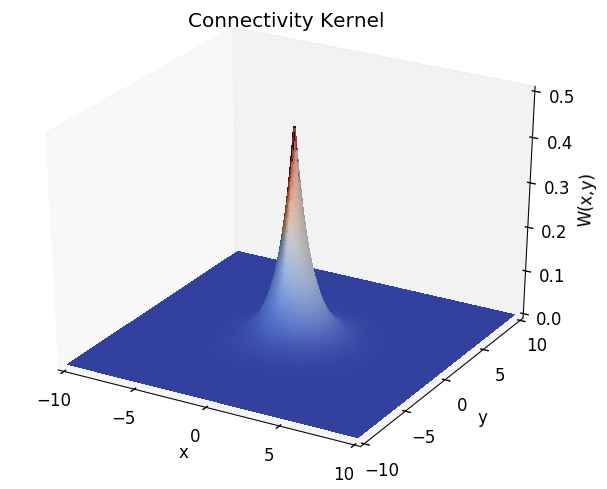
\includegraphics[width=0.5\textwidth]{Figures/2D_Wizard_Hat_Kernel.png}
	\end{center}
	\caption{``Wizard hat" connectivity kernel function given by eqn. \ref{eqn:2d_2component_kernel}}
	\label{fig:2d_2component_kernel}
\end{figure}

Coombes, Schmidt and Avitabile, on the paper \cite{coombes2014spots}, show how this specific model \ref{eqn:2d_2component_gral} with a connectivity kernel that incorporates short range excitation and long range inhibition, and a Heaviside firing rate function $(\mu \rightarrow \infty)$ supports a spot solution whose radius $R$ undergoes a Hopf bifurcation as $h$ is varied, leading to a branch of periodic solutions. On this section we will find this spot solutions with varying radius $R$ by performing simulation with different values of $h$ on different domain intervals $\Omega = [-L,L]^2$. First we solve the model using a Fast Fourier Transform methodology, and then we solve it on a triangulated mesh, as developed in section \ref{sec:nf_t_domain}.

\subsection{Fast Fourier Transform} \label{subsec:adaptation_fft_discretization}
We implement the Fast Fourier Transform method as explained section \ref{subsec:fft} to compute the convolution integral on the right hand side of equation \ref{eqn:2d_2component_gral}.

By writing the integral on the right hand side of eqn.\ref{eqn:2d_2component_gral} as a convolution integral, as defined in \ref{eqn:convolution_definition}, we get
\begin{subequations}\label{eqn:2d_2component_fft}
	\begin{align}
		\frac{1}{\alpha} \frac{\partial u(\textbf{r},t)}{\partial t} &= -u(\textbf{r},t) + W * f(u(\textbf{r},t)) - g a(\textbf{r},t)\\
		\frac{\partial a(\textbf{r},t)}{\partial t} &= -a(\textbf{r},t) + u(\textbf{r},t).
	\end{align}
\end{subequations}

Numerical computations are performed by discretizing a domain $\Omega = [-L,L]^2$ with $n$ evenly-distributed points in each spatial direction and imposing periodic boundary conditions, in such a way that $\Omega_N = \{(x_i, y_j)\}_{i,j=1}^n$, and define a vector $\textbf{u} \in \mathbb{R}^{N}$ such that $\textbf{u}=\{u_{ij}\}_{i,j=1}^N$, with $u_{ij}=u(x_i, y_j)$ and $N=n^2$. Similarly we form vectors $\textbf{w}$, $\textbf{f}(\textbf{u})$, $\textbf{a} \in \mathbb{R}^{N}$ to collect the values of $W$, $f$ and $a$ at each grid point, respectively. Then, the discretized version of \ref{eqn:2d_2component_fft} looks like
\begin{subequations}\label{eqn:2d_2component_fft_discrete}
	\begin{align}
		\dot{\textbf{u}}(t) &= \alpha[\textbf{w} * \textbf{f}(\textbf{u}(t))-\textbf{u}(t) - g\textbf{a}(t)]\\
		\dot{\textbf{a}}(t) &= \textbf{u}(t) - \textbf{a}(t)
	\end{align}
\end{subequations}
  
Now, by using the convolution theorem \ref{eqn: convolution_theorem}, which states that the Fourier transform of a convolution between two functions is the pointwise product of their Fourier transforms, we can compute the integral on the right hand side of \ref{eqn:2d_2component_gral} by computing the Fourier transforms of $\textbf{w}$ and $\textbf{f}(\textbf{u})$, take their pointwise product and then take the inverse Fourier transform of the result. That means
\begin{equation}
 \textbf{w} * \textbf{f}(\textbf{u}) = \mathcal{F}^{-1}_k[\mathcal{F}_k(\textbf{w}) \times \mathcal{F}_k(\textbf{f}(\textbf{u}))].
\end{equation}
In this case, $\mathcal{F}_k(\cdot)$ and $\mathcal{F}^{-1}_k(\cdot)$ are the 2D Discrete Fourier transform (DFT) and its inverse (IDFT), respectively. As mentioned in section \ref{subsec:fft}, one can compute the DFT and the IDFT, with $O(N\log N)$ complexity by using the FFT and IFFT algorithms, respectively. In this case we use the \texttt{fft} and \texttt{ifft} algorithms provided by python \texttt{scipy.fftpack}\footnote{https://docs.scipy.org/doc/scipy/reference/fftpack.html}.

To time step equation \ref{eqn:2d_2component_nystrom} using RK4, we must define a vector $\textbf{v}\in \mathbb{R}^{2N} $ that collects the information of $\textbf{u}$ and $\textbf{a}$, in such a way that $\textbf{v} = [\textbf{u}, \textbf{a}]^T$. So that we can write eqn. \ref{eqn:2d_2component_fft} as
\begin{equation}
\dot{\textbf{v}}(t) = \textbf{F}(\textbf{v}(t)),
\end{equation}
where
\begin{equation}
\textbf{F}(\textbf{v}(t)) = [\alpha(\textbf{w}*\textbf{f}(\textbf{u}(t)) -\textbf{u}(t)-g\textbf{a}(t)), \textbf{u}(t) - \textbf{a}(t)]^T \in \mathbb{R}^{2N}
\end{equation}

\subsection{FFT Results} \label{subsec:adaptation_fft_results}
We present some results of equation \ref{eqn:2d_2component_fft_discrete} after time stepping. In particular, we look at radially-symmetric spot solutions whose radius $R$ changes as the firing threshold parameter $h$ and the length $L$ of the domain interval $\Omega \in [-L, L]^2$ are varied.   

Time simulations are performed over a time interval $t \in [0, 15]$ with steps of $h_t= 0.1$. Initial condition is taken as a Gaussian spot given by

\begin{equation}
	u(\textbf{r}, 0) = u(x,y) = 6\exp{\left(-\frac{x^2+y^2}{5.77}\right)}.
\end{equation}
Further, we take $g=1$, $\alpha=1.2$, and work with a Heaviside firing rate by taking $\mu=50$ (big).

First, we work on the domain interval $\Omega \in [-80, 80]^2$. Figure \ref{fig:adapt_fft_L_80} shows the radially-symmetric spot solution at final time $t=15$, with different radius $R$ for varying cases of $h$ on each row. At $h=0.4$ a spot solution with radius $R \approx 60$ is formed, a smaller circle with radius $R \approx 40$ is formed in the case $h=0.5$, and we note how, on the case $h=0.6$ the spot solution is destroyed. That means, we get a steady state $u \equiv 0$. However, is we reduce the size of the interval, we can get a spot solution for the case $h=0.6$.

Figure \ref{fig:adapt_fft_L_60} show the spot solutions at final time $t=15$, on a domain interval $\Omega \in [-60, 60]^2$ for different cases of $h$ in each row. Note how, when $h=0.5$, the spot solution with $R\approx40$ is formed. When $h=0.6$, a spot solution with $R\approx20$ is displayed, and no spot solution is formed when $h=0.7$ ($u \equiv 0$).

It is worth noting that, further reducing the interval length $L$ does not cause another spot solution to be formed when $h \geq 0.7$. However, spot solutions with bigger radius $R$ can be found by taking a bigger interval length $L > 80$ and values of $h \in (0,0.4)$.
\begin{figure}
	\begin{center}
		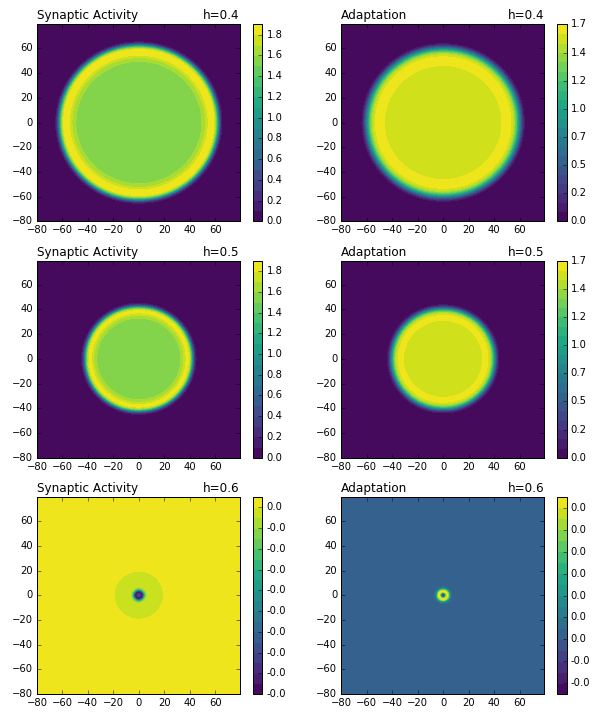
\includegraphics[width=0.8\textwidth]{Figures/AdaptFFT_L=80.png}
	\end{center}
	\caption{Radially symmetric spot solutions at final time $t=15$ for different values of $h$ on each row using the FFT method on a grid $[-80, 80]^2$. On the first row, with $h=0.4$, a spot solution of $R \approx 60$ is displayed, on the second row, using $h=0.5$, a spot solution with $R \approx 40$ is shown, and the third case, $h=0.6$, is a flat state.}
	\label{fig:adapt_fft_L_80}
\end{figure}

\begin{figure}
	\begin{center}
		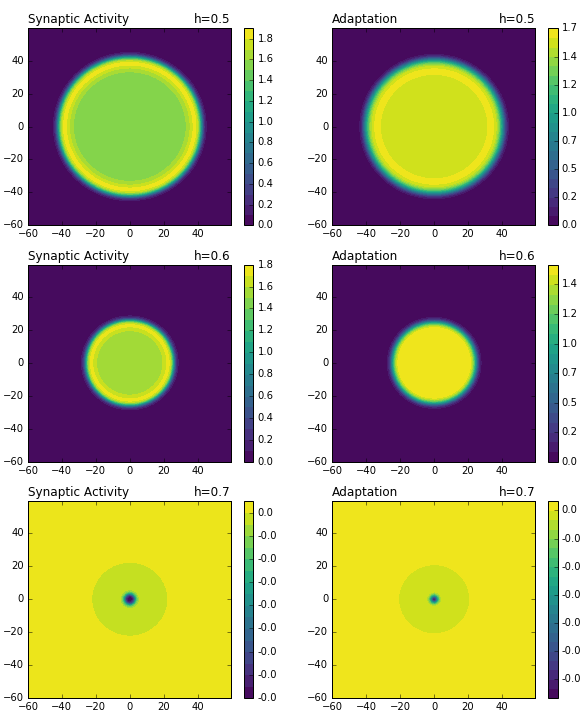
\includegraphics[width=0.8\textwidth]{Figures/AdaptFFT_L=60.png}
	\end{center}
	\caption{Radially symmetric spot solutions at final time $t=15$ for different values of $h$ on each row using the FFT method on a grid $[-60, 60]^2$. On the first row, with $h=0.5$, a spot solution of $R \approx 40$ is displayed, on the second row, using $h=0.6$, a spot solution with $R \approx 20$ is shown, and the third case, $h=0.7$, is a flat state.}
	\label{fig:adapt_fft_L_60}
\end{figure}

\subsection{Nystr\"om on a Triangulated Mesh}
\label{subsec:adaptation_triMesh_discretization}
To discretize the right hand side of equation \ref{eqn:2d_2component_gral} we use Nystr\"om method with a Gaussian quadrature rule as developed in section \ref{subsec:tri nystrom discretize}. In other words, the discretized equation looks like
\begin{subequations}\label{eqn:2d_2component_nystrom}
	\begin{align}
		\dot{\textbf{u}}(t) &= \alpha[\textbf{W}\textbf{f}(\textbf{u}(t)) -\textbf{u}(t)-g\textbf{a}(t)]\\
		\dot{\textbf{a}}(t) &= \textbf{u}(t) - \textbf{a}(t) 		 ,
	\end{align}
\end{subequations}
where $\textbf{W}$ and $\textbf{f}$ are defined as in eqn. \ref{eqn:2d_tri_w&f}, on a triangulated domain $\Omega_h$ with $[-L,L]$ limits. To time step equation \ref{eqn:2d_2component_nystrom} using RK4, we must define a vector $\textbf{v} \in \mathbb{R}^{2N}$ that contains the information of $\textbf{u}$ and $\textbf{a}$, such that $\textbf{v} = [\textbf{u}, \textbf{a}]^T$. So that we can write eqn. \ref{eqn:2d_2component_nystrom} as
\begin{equation}
	\dot{\textbf{v}}(t) = \textbf{F}(\textbf{v}(t)),
\end{equation}
where
\begin{equation}
\textbf{F}(\textbf{v}(t)) = [\alpha(\textbf{W}\textbf{f}(\textbf{u}(t)) -\textbf{u}(t)-g\textbf{a}(t)), \textbf{u}(t) - \textbf{a}(t)]^T \in \mathbb{R}^{2N}
\end{equation}

\subsection{Triangulated Mesh Results} \label{sebsec:adaptation_triMesh_results}
We compare the results obtained using the methodology on section \ref{subsec:adaptation_triMesh_discretization}, with the results using the FFT method in section \ref{subsec:adaptation_fft_results}, after time stepping.

Time simulations are performed over a time interval $t \in [0, 15]$ with steps of $h_t= 0.1$. Initial condition is taken as a Gaussian spot given by

\begin{equation}
u(\textbf{r}, 0) = u(x,y) = 6\exp{\left(-\frac{x^2+y^2}{5.77}\right)}.
\end{equation}
Further, we take $g=1$, $\alpha=1.2$, and work with a Heaviside firing rate by taking $\mu=50$ (big). First we work on a triangulated domain $\Omega$ with limits $[-80,80]$ to generate the spot solutions for the cases $h=0.4$ and $h=0.5$ as in figure \ref{fig:adapt_fft_L_80}. Then we decrease the domain limits to $[-30,30]$ in order to generate the spot solution when $h=0.6$, as the one in figure \ref{fig:adapt_fft_L_60}, second row. 

Figure \ref{fig:tri_mesh_adapt_p4h} shows a radially-symmetric spot solution with radius $R \approx 60$ when $h=0.4$ on a triangulated domain $\Omega_h \in [-80,80]$, as the one shown in figure \ref{fig:adapt_fft_L_80}, first row. 

Figure \ref{fig:tri_mesh_adapt_p5h} displays another radially-symmetric spot solution with radius $R \approx 40$ when $h=0.5$ on the same domain, as the one generated in figure \ref{fig:adapt_fft_L_80}, second row. 

To generate the spot solution for the case $h=0.6$ we must reduce the domain limits, figure \ref{fig:tri_mesh_adapt_p6h} shows the radially-symmetric spot solution with radius $R \approx 20$ for this case ($h=0.6$), on a triangulated domain $\Omega_h \in [-30,30]$, as the one shown in figure \ref{fig:adapt_fft_L_60}, second row. 

Again, it is worth noting that, for smaller values of $h \in (0, 0.4)$, bigger spot solutions can be found. To generate these solutions one must increase the domain, which also increases the number of elements, and therefore, generating this bigger circles becomes extremely slow. Additionally, for values $h \leq 0.7$ a flat state $u \equiv 0$ is generated no matter how much we reduce the domain length $L$.

\begin{figure}
	\begin{center}
		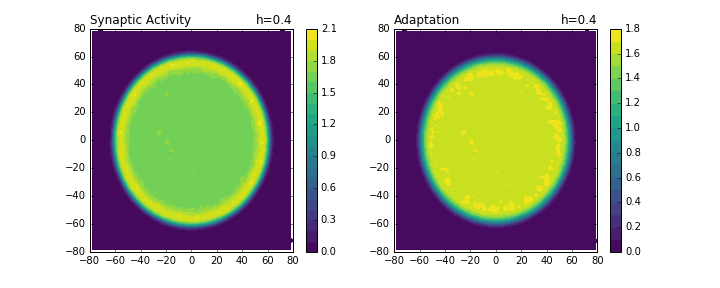
\includegraphics[width=0.8\textwidth]{Figures/Adapt_8838elems_(p4)h.png}
	\end{center}
	\caption{Radially-symmetric spot solution with radius $R\approx 60$, at final time $t=15$, for the case $h=0.4$, on a triangulated mesh $\Omega$ between $[-80,80]^2$ comprised of $N_t=8,838$ triangular elements and $N_g=3$ interior Gauss points.}
	\label{fig:tri_mesh_adapt_p4h}
\end{figure}

\begin{figure}
	\begin{center}
		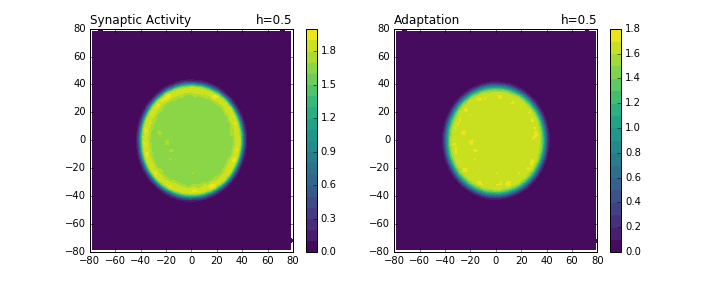
\includegraphics[width=0.8\textwidth]{Figures/Adapt_8838elems_(p5)h.png}
	\end{center}
	\caption{Radially-symmetric spot solution with radius $R\approx 50$, at final time $t=15$, for the case $h=0.5$, on a triangulated mesh $\Omega$ between $[-80,80]^2$ comprised of $N_t=8,838$ triangular elements and $N_g=3$ interior Gauss points.}
	\label{fig:tri_mesh_adapt_p5h}
\end{figure}

\begin{figure}
	\begin{center}
		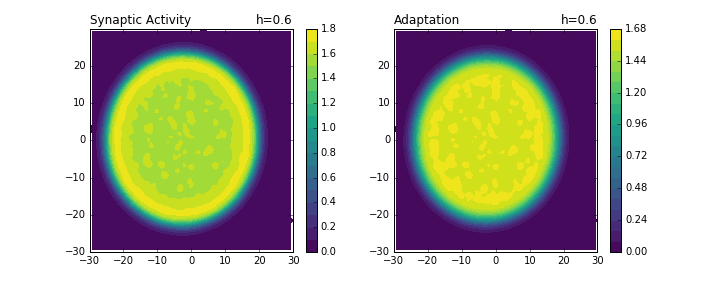
\includegraphics[width=0.8\textwidth]{Figures/Adapt_2746elems_(p6)h.png}
	\end{center}
	\caption{Radially-symmetric spot solution with radius $R\approx 20$, at final time $t=15$, for the case $h=0.6$, on a triangulated mesh $\Omega$ between $[-30,30]^2$ comprised of $N_t=2,746$ triangular elements and $N_g=3$ interior Gauss points.}
	\label{fig:tri_mesh_adapt_p6h}
\end{figure}
%--------------------------------------
\section{Jupyter Notebook} \label{sec:jupyter_notebook}
On this section we include the Jupyter Notebooks used to solve the 2D neural field model on a triangulated mesh as in section \ref{sec:nf_t_domain}.
\subsection{2D Model in a Triangulated Mesh}
In this script we solve a Wilson-Cowan-Amari neural field equation on a
two dimensional triangulated mesh \(\Omega \in \mathbb{R}^2\), where we
discretize \(\Omega\) with \(N_t\) triangular elements \(\kappa\), such
that \(\Omega \approx \Omega_h = \bigcup_{i=1}^{N_t} \kappa_{i}.\\\)

The equation looks like:

\begin{equation}
\frac{\partial u(\mathbf{x},t)}{\partial t} = - u(\mathbf{x},t) + \int_{\Omega} w(\mathbf{x}-\mathbf{y})f(u(\mathbf{y}, t)) d\mathbf{y}, \hspace{3mm} \mathbf{x}, \mathbf{y} \in \mathbb{R}^2, t \in \mathbb{R}^+,
\end{equation}

where \(u(\mathbf{x},t)\) is the synaptic activity,
\(w(\mathbf{x}-\mathbf{y})\) the synaptic connectivity kernel and
\(f(u)\) a non-linear function for the conversion of the synaptic
potential into a firing rate. In general, both \(w\) and \(f\) depend
upon control parameters which are defined later.

\subsubsection{Choices for the Connectivity Kernel and Firing Rate Function:}\label{choices-for-the-connectivity-kernel-and-firing-rate-function}

The Connectivity Kernel and Firing Rate Function are objects that
receive the Parameters on their Constructors and can be evaluated using
the ( ) operator. For instance, a user can define a personalized kernel
or firing rate function. They are defined as:\\
Connectivity Kernel1:

\[ w(\textbf{x};b) = \frac{1}{2} e^{-b||\textbf{x}||}\\\] Connectivity
Kernel2:

\[ w(\textbf{x}; b) = e^{-b||\textbf{x}||}(b \sin{||\textbf{x}||} + \cos{||\textbf{x}||}) \\\]
Here, \(b\) controls the decay of the oscillatory behaviour of the
Synaptic Kernel.\\
Firing Rate1:

\[ f(u; \mu, \theta) = \frac{1}{1+exp(-\mu(u-\theta))} \\\] Firing
Rate2:

\[ f(u; \mu, \theta) = \frac{1}{1+e^{-\mu u + \theta}} - \frac{1}{1+e^\theta}\\\]
Here, \(\mu\) controls the slope of the sigmoidal firing rate, and
\(\theta\) is a threshold value.

\begin{minted}{python}
import numpy as np
from meshtools import *
import NeuralField as nf
import ConnectivityKernel as ck
import FiringRate as fr
import QuadratureInTriangles as Qtri
import InitialConditions as ic
import matplotlib.pyplot as plt
from scipy.integrate import ode
from matplotlib.mlab import griddata
%matplotlib inline
\end{minted}

\begin{minted}{python}
# Used for Plotting 3D result with linear vectors
def toMeshGrid(x, y, z, resX=100, resY=100):
	"Convert 3 column data to matplotlib meshgrid"
	xi = np.linspace(min(x), max(x), resX)
	yi = np.linspace(min(y), max(y), resY)
	Z = griddata(x, y, z, xi, yi)
	X, Y = np.meshgrid(xi, yi)
	return X, Y, Z
\end{minted}

\begin{minted}{python}
# Generate Mesh
Lx=-30; Ux=30
Ly=-30; Uy=30
length = 3 # Decrease length to increase number of elements
p,v=RectangleSegments([Ux,Uy],[Lx, Ly],edge_length=length)
mesh_pts, elems = DoTriMesh(p,v,edge_length=length)
NT = len(elems) # Number of triangles
print("Number of Elements = " + str(NT))
\end{minted}
Number of Elements = 1234


\begin{minted}{python}
# plot mesh
plot_mesh = True
if(plot_mesh):
	fig1 = plt.figure()
	fig1.suptitle("Triangulated Mesh")
	ax = fig1.add_subplot(111)
	ax.triplot(mesh_pts[:, 0], mesh_pts[:, 1], elems)
	ax.set_xlabel("x")
	ax.set_ylabel("y")
	fig1.savefig("The_Mesh")
\end{minted}

\begin{figure}[H]
	\centering
	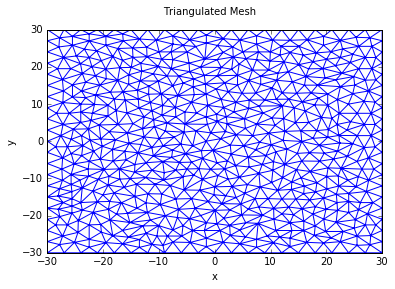
\includegraphics[width=0.6\textwidth]{2dNystTriang_Main_files/2dNystTriang_Main_5_0.png}
	\caption{Triangulated mesh}
\end{figure}

\begin{minted}{python}
Np = 2 # Degree of precision

gwp = Qtri.getWeightsAndPoints(Np)

x_hat = gwp[:,0]
y_hat = gwp[:,1]
weights = gwp[:,2]

Ng = len(weights) # Number of Gauss interior points.

print("x_hat = "+str(x_hat))
print("y_hat = "+str(y_hat))
print("wgts = "+str(weights))

\end{minted}
x\_hat = [ 0.16666667  0.16666667  0.66666667]\\
y\_hat = [ 0.16666667  0.66666667  0.16666667]\\
wgts = [ 0.33333333  0.33333333  0.33333333]

\begin{minted}{python}
# Assemble Mesh of Interior Points
xs = []
As = []
for l, elem in enumerate(elems):
	v1,v2,v3 = mesh_pts[elem] # Get vertices of the element
	A_l = Qtri.computeArea(v1,v2,v3)
	As.append(A_l)
	for j in range(len(weights)):
		new_point = Qtri.mapX(v1, v2, v3, x_hat[j], y_hat[j])
		xs.append(new_point)
xs = np.array(xs)
As = np.array(As)
N = len(xs)
\end{minted}

\begin{minted}{python}
# Visualize interior points
visualize = False # Change flag if you want to visualize the mesh with interior points
if(visualize):
	fig2 = plt.figure(figsize = (9,6))
	fig2.suptitle("Triangulated Mesh with " +str(Ng)+" Interior Gauss Points")
	ax = fig2.add_subplot(111)
	ax.triplot(mesh_pts[:, 0], mesh_pts[:, 1], elems)
	for p in xs:
		ax.plot([p[0]],[p[1]], 'r.')
	ax.set_xlabel("x")
	ax.set_ylabel("y")
	fig2.savefig("Mesh With "+str(Ng)+" Interior Points")
\end{minted}

\begin{minted}{python}
# Initialize Connectivity Kernel
b = 0.4
kernel = ck.ConnectivityKernel2(b)
\end{minted}

\begin{minted}{python}
# Assemble Synaptic Matrix
wts_o = np.outer(As.T, weights)
rhos = wts_o.flatten()

W = np.zeros((N,N))
for i in range(0, N):
	x_pt = xs[i]
	for j in range(i, N):
		y_pt = xs[j]
		x, y = x_pt-y_pt
		W[i,j] = kernel(x, y) 

# Copy upper triangular part to lower triangular part
i_lower = np.tril_indices(N, -1)
W[i_lower] = W.T[i_lower]

# Multiply times the weights
W *= rhos
del rhos # delete to free memory
\end{minted}

\subsubsection{Time step using standard ODE solvers}\label{time-step-using-standard-ode-solvers}

\begin{minted}{python}
# Parameters for Firing Rate
mu = 3.2; theta = 5.6;
f_rate = fr.FiringRate2(mu, theta)

# Initialize Neural Field
NeuralField = nf.NeuralField(f_rate, W)
\end{minted}

\begin{minted}{python}
# Initial Conditions
#_A = 6; _L = 5.77 # parameters for initial condition 1
_A = 2; _L = 100 # parameters for initial condition 2
initCond = ic.InitialCondition2(_A, _L)

u0 = []
for point in xs:
	x,y = point
	u0.append(initCond(x,y))
u0 = np.array(u0)
\end{minted}

\begin{minted}{python}
method = ode(NeuralField).set_integrator("dopri5")
method.set_initial_value(u0)
final_t = 15
dt = 0.1
us = []
time_points = []
while method.t < final_t:
	next_t = method.t+dt
	time_points.append(next_t)
	next_u = method.integrate(next_t)
	us.append(next_u)
\end{minted}

\subsubsection{Plot Solution}\label{plot-solution}

\begin{minted}{python}
fig = plt.figure(figsize=(15,3))

# Plot initial time
ax1 = fig.add_subplot(131)
xx0, yy0, uu0 = toMeshGrid(xs[:,0], xs[:,1], u0)
cont1 = ax1.contourf(xx0, yy0, uu0, 20, cmap=plt.get_cmap('viridis'))
ax1.set_title("t = 0", loc="left")
ax1.set_title(r'$\mu =$'+str(mu), loc="right")
plt.colorbar(cont1)

# Plot half time
ax2 = fig.add_subplot(132)
xn_2, yn_2, un_2 = toMeshGrid(xs[:,0], xs[:,1], us[int(len(time_points)/2)])
cont2 = ax2.contourf(xn_2, yn_2, un_2, 20, cmap=plt.get_cmap('viridis'))
ax2.set_title("t = "+str(int(final_t/2)), loc="left")
ax2.set_title(r'$\mu =$'+str(mu), loc="right")
plt.colorbar(cont2)

# Plot final time
ax3 = fig.add_subplot(133)
xn, yn, un = toMeshGrid(xs[:,0], xs[:,1], us[-1])
cont3 = ax3.contourf(xn, yn, un, 20, cmap=plt.get_cmap('viridis'))
ax3.set_title("t = "+str(final_t), loc="left")
ax3.set_title(r'$\mu =$'+str(mu), loc="right")
plt.colorbar(cont3)
plt.savefig("Plots/IC"+str(initCond.num)+"/2dTri_IC"+str(initCond.num)+str(NT)+"_elems_("+str(mu)+")mu.png")
\end{minted}

\begin{figure}[H]
	\centering
	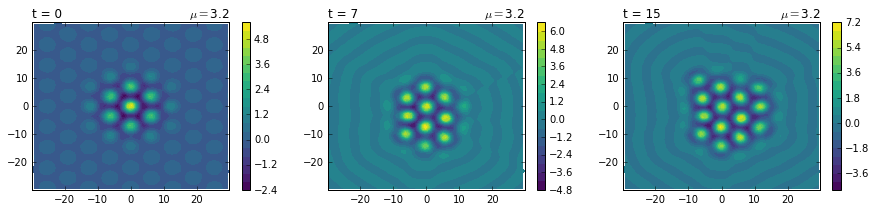
\includegraphics[width=1\textwidth]{2dNystTriang_Main_files/2dNystTriang_Main_16_0.png}
	\caption{Synaptic Activity}
\end{figure}



%---------------------------------------
\section{Conclusions} \label{sec:conclusions}

Over the course of this work we developed a numerical method that solves neural field equations on triangulated meshes by using Nystr\"om method with Gaussian quadrature. Additionally, we produced object oriented code in python for solving different instances of the neural field equation for a variety of connectivity kernel and firing rate functions with different parameters and initial conditions.

In general, we found that by pre-building a Synaptic Matrix which holds the interactions between neurons mediated by the connectivity kernel function one can perform faster right hand side evaluations of the system and work with finer meshes. However, even though we devised a strategy that halves the time it takes to assemble the matrix, and which allowed us to work with finer meshes, we still found this approach to be memory and time consuming when working with refined or big meshes.

When we applied the Nystr\"om method to the one dimensional case, we found localised bump solutions in accordance to previous studies like \cite{LaingCarloR.2002MBia,rankin2014continuation}. Particularly, we found that by setting the firing parameter on an interval, and by varying the initial condition we are able to produce different bump solutions.

On the two dimensional case we found results in accordance to Rankin and Avitabile paper \cite{rankin2014continuation} page 4. We saw how changes in the slope of the sigmoidal firing rate affect the stability of the solutions, leading to other localised states or to domain-covering patterns.

When validating this same results for the two dimensional case on a triangulated mesh we found that the convergence of spot solutions is extremely sensitive to mesh discretizations and thus, a very fine mesh is required to accurately compute solutions of neural field models. This result goes in accordance with Rankin and Avitabile \cite{rankin2014continuation} where they show that the choice of the connectivity kernel function has a considerable impact on the stability properties and on the evolution of the localised states. In particular, a less refined mesh amounts to having a more sparse connectivity structure, meaning that groups of neurons are less connected between them, which is equivalent to changing the connectivity kernel function. Therefore, using a less refined mesh affects the stability properties and the evolution of the localised states.

On the two dimensional case with adaptation we compared the results obtained by solving the system on a tensor product grid using a Fast Fourier Transform method with the results obtained by solving the system on a triangulated mesh using Nystr\"om method with a Gaussian quadrature. Particularly, based on the work of \cite{coombes2014spots}, we found radially-symmetric spot solutions whose radius varies as the firing threshold parameter is varied. When solving the system with the Fast Fourier Transform method we found that the spot solution follows a bifurcation diagram as the one in \cite{coombes2014spots} figure 7.3, where we found the radius of the spot solution to decrease as the firing threshold parameter is decreased until the spot solution is destroyed, in which case we get a flat state. When solving the system on a triangulated mesh with Nystr\"om method, we realised that we needed a very fine grid to reproduce the spot solutions with bigger radius. This caused the algorithm to become very slow.

A most accurate way to simulate synaptic activity might be to get the interaction between neurons from experimental studies, and store them inside the synaptic matrix. However, this would require working with big matrices.

As mentioned earlier, a limitation from working with matrices for developing the numerical methods is that an additional $O(N^2)$ memory is required for storing the matrix. Besides, for more refined grids, or too big domains, this approach proved to be memory and time consuming.

Therefore, there is a need for methods that can handle faster right hand side evaluations of the system and that can perform efficiently on finer meshes without working with matrices. A possible solution, and hence an extension of this work, might be to implement an iterative for loop strategy with parallel algorithms, or to store the interactions between neurons in a graph and efficiently traverse it, or traverse it with parallel algorithms.

The work developed here might be recovered to develop numerical methods that solve the neural field equation on a triangulated surface manifold that more closely resembles the bumps and grooves that are present on a real brain.

\newpage

\appendix

\section{Appendix Code} \label{app:code}

\subsection{Connectivity Kernel Class} \label{app:connectivity_kernel}
\begin{minted}{python}
"""
Various choices for Connectivity Kernels.
They are callable objects and work for 1D or 2D cases.

1D Example:
kernel = ConnectivityKernel1(b=0.1)
x=1
result = kernel(x)

2D Example:
kernel = ConnectivityKernel1(b=0.1)
x=1; y=2
result = kernel(x,y)
"""

import numpy as np

class AbstractConnectivityKernel:
	"""
	AbstractConnectivityKernel Object
	-------------------
	Encapsulates the Parameters of the Connectivity Kernel function for a 
	Neural Field Integral model.
	"""
	def __init__(self, b=1):
		"""
		Constructor
		--------------------
		Receives:
			b -> Parameter that controls the decay rate of
				the Connectivity Kernel.
				b=1 by default (when no decay parameter).
		"""
		self.b = b

class ConnectivityKernel1(AbstractConnectivityKernel):
	"""
	ConnectivityKernel1 Object "Wizard Hat"
	-------------------
	Inherits data from AbstractConnectivityKernel 
	"""
	def __call__(self, x, y=0):
		"""
		operator ()
		----------------------------------------
		Evaluate the Connectivity Kernel Function 
		at the given x,y coordinates
		"""
		nrm = np.sqrt(x*x + y*y) # Euclidian norm
		
		return 0.5*np.exp(-self.b*nrm)

class ConnectivityKernel2(AbstractConnectivityKernel):
	"""
	ConnectivityKernel2 Object "Mexican Hat"
	-------------------
	Inherits data from AbstractConnectivityKernel 
	"""
	def __call__(self, x, y=0):
		"""
		operator ()
		----------------------------------------
		Evaluate the Connectivity Kernel Function 
		at the given x,y coordinates
		"""
		nrm = np.sqrt(x*x + y*y) # Euclidian norm
		return np.exp( -self.b*nrm )*( self.b*np.sin(nrm) + np.cos(nrm) )
\end{minted}
\subsection{Firing Rate Class} \label{app:firing_rate}
\begin{minted}{python}
"""
Various choices for Firing Rate function. They are callable objects
and work for 1D and 2D cases.

Example:
firing_rate = FiringRate1(mu=3.5, theta=5.6)
random_dim = np.random.randint(1,50)
u = np.zeros( random_dim )
result = firing_rate(u)
"""
	
import numpy as np
	
class AbstractFiringRate:
	"""
	AbstractFiringRate Object
	-------------------
	Encapsulates the Parameters of the Firing Rate function for a 
	Neural Field Integral model.
	"""
	def __init__(self, slope, threshold):
		"""
		Constructor
		-------------------
		Receives:
			slope -> Slope of the sigmoid function (float)
			threshold -> Firing threshold value (float)
		"""
		self.mu = slope
		self.theta = threshold
	
class FiringRate1(AbstractFiringRate):
	"""
	FiringRate1 Object
	-------------------
	Inherits data from AbstractFiringRate 
	"""
	def __call__(self, u):
		"""
		operator ()
		--------------------------------------
		Evaluate the Firing Rate Function at the
		given u (u might be a vector or an integer).
		"""
		m = self.mu; h = self.theta
		return 1 / (1 + np.exp(- m * (u - h) ))
	
class FiringRate2(AbstractFiringRate):
	"""
	FiringRate2 Object
	-------------------
	Inherits data from AbstractFiringRate 
	"""
	def __call__(self, u):
		"""
		operator ()
		--------------------------------------
		Evaluate the Firing Rate Function at the
		given u (u might be a vector or an integer).
		"""
		m = self.mu; h = self.theta
		return 1/( 1 + np.exp(- m*u + h) ) - 1/( 1 + np.exp(h) )
\end{minted}

\subsection{Neural Field Class} \label{app:neural_field}
\begin{minted}{python}
"""
NeuralField Object
--------------------
Discretized Amari type Neural Field Integral equation.
Uses a synaptic matrix assembled by the Nystrom Method.
"""
	
import numpy as np
	
class NeuralField:
	
	def __init__(self, firing_rate, synaptic_matrix):
		"""
		Constructor
		---------------------------------
		Receives:
			firing_rate -> callable object or callable function 
			synaptic_matrix -> Square matrix (Synaptic connectivity)
		"""
		self.W = synaptic_matrix
		self.f_rate = firing_rate
	
	def __call__(self, t, u):
		"""
		operator ()
		--------------------
		Evaluate the discretized integral equation
		at the given time t and vector u.
		* Can be used directly with time steppers.
		"""
		f_u = self.f_rate(u) # Evaluate firing rate at u.
		return -u + (self.W).dot(f_u)
\end{minted}

\subsection{Neural Field With Adaptation Class} \label{app:nf_with_adaptation}
\begin{minted}{python}
"""
NeuralField Object
--------------------
Neural Field model with linear spike frequency adaptation
as the one in the paper: "Spots: Breathing, Drifting and 
Scattering in a Neural Field Model" by Coombes, Schmidt
and Avitabile
"""

import numpy as np

class NeuralFieldWithAdaptation:

	def __init__(self, firing_rate, synaptic_matrix, alpha, g):
		"""
		Constructor
		---------------------------------
		Receives:
			firing_rate -> callable object or callable function 
			synaptic_matrix -> Square matrix (Synaptic connectivity)
			alpha -> Adaptation constant
			g -> Strength of the negative feedback
		"""
		self.f_rate = firing_rate
		self.W = synaptic_matrix
		self.alpha = alpha
		self.g = g
	
	def __call__(self, t, v):
		"""
		operator ()
		--------------------
		Evaluate the discretized integral equation
		at the given time t and vector u.
		* Can be used directly with time steppers.
		"""
		alpha = self.alpha; g = self.g
		N = int( len(v)/2 )
		u = v[:N]; a=v[N:] # Break v in u and a
		
		f_u = self.f_rate(u) # Evaluate firing rate at u
		v0 = alpha*( (self.W).dot(f_u) - u - g*a ) # Equate synaptic activity
		v1 = u - a # Equate adapative field
		
		result = np.concatenate([v0,v1]) # stack v0 on top of v1
		
		return result
\end{minted}

\subsection{Initial Conditions Class} \label{app:initial_conditions}
\begin{minted}{python}
"""
Various choices of Initial Conditions for time stepping.
See: CONTINUATION OF LOCALISED COHERENT STRUCTURES IN NONLOCAL NEURAL FIELD 
EQUATIONS, JAMES RANKIN and DANIELE AVITABILE. Appendix A, page 19.
"""
import numpy as np
	
class InitialCondition1():
	
	def __init__(self, A, L):
		"""
		Constructor
		--------------------
		Receives:
			A -> Amplitud; L -> Length or "kurtosis"
		"""
		self._A = A; self._L = L; self.num = 1
	
	def __call__(self, x,y):
		"""
		operator ()
		---------------------------------
		Evaluate the initial condition function at
		the given point with x,y coordinates
		"""
		e = np.exp(-(x**2 + y**2)/self._L)
		return self._A*e
	
class InitialCondition2():
	
	def __init__(self, A, L):
		"""
		Constructor
		--------------------
		Receives:
			A -> Amplitud; L -> Length or "kurtosis"
		"""
		self._A = A; self._L = L; self.num = 2
	
	def __call__(self, x,y):
		"""
		operator ()
		---------------------------------
		Evaluate the initial condition function at
		the given point with x,y coordinates
		"""
		e = np.exp(-(x**2 + y**2)/self._L)
		cos1 = np.cos(x)
		cos2 = np.cos( 0.5*x + (np.sqrt(3)/2)*y )
		cos3 = np.cos( -0.5*x + (np.sqrt(3)/2)*y )
		return self._A*e*(cos1 + cos2 + cos3)
\end{minted}

\subsection{Gaussian Quadrature on Triangulated Mesh} \label{app:gauss_quad}
\begin{minted}{python}
import numpy as np
from GaussWeightsPoints import getWeightsAndPoints
from meshtools import *
import matplotlib.pyplot as pt
from mpl_toolkits.mplot3d import Axes3D
import numpy as np
import matplotlib.pyplot as pt

# Nodal Basis Functions for Mapping points in a canonical 
# reference element to an element in the mesh.
N1 = lambda x_hat, y_hat: 1 - x_hat - y_hat
N2 = lambda x_hat, y_hat: x_hat
N3 = lambda x_hat, y_hat: y_hat

# Function that maps any point in the element K using its vertices and
# the coordinates of that point inside a reference triangle
def mapX(v1, v2, v3, x_hat, y_hat):
	"""
	v1, v2, v3 are lists containing x and y
	i.e. v1 = [x1, y1],
	and represent the vertices of a triangular element.
	x_hat is the x value of a point inside the refernce triangle
	y_hat is the y value of a point inside the reference triangle
	"""
	# Map gauss points inside the triangle using the Nodal Basis Functions
	x = v1[0]*N1(x_hat, y_hat) + v2[0]*N2(x_hat, y_hat) + v3[0]*N3(x_hat, y_hat)
	y = v1[1]*N1(x_hat, y_hat) + v2[1]*N2(x_hat, y_hat) + v3[1]*N3(x_hat, y_hat)
	return np.array([x, y])

def computeArea(v1, v2, v3):
	x1, y1 = v1; x2, y2 = v2; x3, y3 = v3;
	A = abs( x1*(y2-y3) + x2*(y3-y1) + x3*(y1-y2) )/2.0
	return A

def gaussIntTriangle(f, N_point, v1, v2, v3):
	""" 
	Evaluates \int \int_K f(x,y) dxdy
	using a Gaussian Quadrature of order N,
	where K is a triangle with vertices at
	v1,v2,v3. 
	Each vertex v is a 2D array containing
	its x and y coordinates. i.e.
	v = [x, y]
	"""
	xw = getWeightsAndPoints(N_point) # Get quadrature points and weights.
			
	#Calculate the area of the Triangle.
	A = computeArea(v1,v2,v3)
	
	# Weights and points on the reference triangle
	x_hat = xw[:,0]
	y_hat = xw[:,1]
	weights = xw[:,2]
	
	# number of Gauss points
	np = len(weights)
	
	result = 0
	for i in range(np):
	# Map interior points to the element.
		x, y = mapX(v1,v2,v3, x_hat[i], y_hat[i])
		result += f(x,y)*weights[i]
	
	result *= A		
	return result

def main():

	# Create triangulated mesh
	edge_length = 0.3
	p, v = RectangleSegments([2,2],[-2,-2], edge_length=edge_length)
	mesh_pts, elems = DoTriMesh(p, v, edge_length)
	
	# Function to integrate over 
	def f(x, y): return x**2 + y**2
	
	# Compute Integral over the T mesh
	N = 2 # Point rule of the Quadrature
	S = 0
	# Iterate through each element
	for i, elem in enumerate(elems):
		# Get vertices of the element
		v1,v2,v3 = mesh_pts[elem]
		# Compute the integral of each element.
		S += gaussIntTriangle(f, N, v1, v2, v3)
		
	print("Result: " +str(S))
	print("Error: " + str(S - 128/3))

if __name__ == "__main__": main()
\end{minted}
\subsection{Gaussian Weights and Points on Triangular Element} \label{app:gauss_ws_and_ps}
\begin{minted}{python}
from numpy import array

def getWeightsAndPoints(n):
	if (n == 1):
		xw=[1/3, 1/3, 1]
	elif (n == 2):
		xw=[[1/6, 1/6, 1/3],
			[1/6, 2/3, 1/3], 
			[2/3, 1/6, 1/3]]
	elif (n == 3):
		xw=[[1/3, 1/3, -27/48],
			[3/5, 1/5, 25/48],
			[1/5, 1/5, 25/48],
			[1/5, 3/5, 25/48]]
	elif (n == 4):
		xw=[[0.44594849091597, 0.44594849091597, 0.22338158967801],
			[0.44594849091597, 0.10810301816807, 0.22338158967801],
			[0.10810301816807, 0.44594849091597, 0.22338158967801], 
			[0.09157621350977, 0.09157621350977, 0.10995174365532], 
			[0.09157621350977, 0.81684757298046, 0.10995174365532], 
			[0.81684757298046, 0.09157621350977, 0.10995174365532]]
	else:
	print("Haven't computed points for that degree.")
	xw = np.zeros(n, 3)
	
	return array(xw)
	
\end{minted}

%----------------------------
\newpage
\bibliography{mybibliography}

\end{document}
